% Options for packages loaded elsewhere
\PassOptionsToPackage{unicode}{hyperref}
\PassOptionsToPackage{hyphens}{url}
\PassOptionsToPackage{dvipsnames,svgnames,x11names}{xcolor}
%
\documentclass[
]{article}
\usepackage{amsmath,amssymb}
\usepackage{iftex}
\ifPDFTeX
  \usepackage[T1]{fontenc}
  \usepackage[utf8]{inputenc}
  \usepackage{textcomp} % provide euro and other symbols
\else % if luatex or xetex
  \usepackage{unicode-math} % this also loads fontspec
  \defaultfontfeatures{Scale=MatchLowercase}
  \defaultfontfeatures[\rmfamily]{Ligatures=TeX,Scale=1}
\fi
\usepackage{lmodern}
\ifPDFTeX\else
  % xetex/luatex font selection
\fi
% Use upquote if available, for straight quotes in verbatim environments
\IfFileExists{upquote.sty}{\usepackage{upquote}}{}
\IfFileExists{microtype.sty}{% use microtype if available
  \usepackage[]{microtype}
  \UseMicrotypeSet[protrusion]{basicmath} % disable protrusion for tt fonts
}{}
\makeatletter
\@ifundefined{KOMAClassName}{% if non-KOMA class
  \IfFileExists{parskip.sty}{%
    \usepackage{parskip}
  }{% else
    \setlength{\parindent}{0pt}
    \setlength{\parskip}{6pt plus 2pt minus 1pt}}
}{% if KOMA class
  \KOMAoptions{parskip=half}}
\makeatother
\usepackage{xcolor}
\usepackage[margin=1in]{geometry}
\usepackage{longtable,booktabs,array}
\usepackage{calc} % for calculating minipage widths
% Correct order of tables after \paragraph or \subparagraph
\usepackage{etoolbox}
\makeatletter
\patchcmd\longtable{\par}{\if@noskipsec\mbox{}\fi\par}{}{}
\makeatother
% Allow footnotes in longtable head/foot
\IfFileExists{footnotehyper.sty}{\usepackage{footnotehyper}}{\usepackage{footnote}}
\makesavenoteenv{longtable}
\usepackage{graphicx}
\makeatletter
\def\maxwidth{\ifdim\Gin@nat@width>\linewidth\linewidth\else\Gin@nat@width\fi}
\def\maxheight{\ifdim\Gin@nat@height>\textheight\textheight\else\Gin@nat@height\fi}
\makeatother
% Scale images if necessary, so that they will not overflow the page
% margins by default, and it is still possible to overwrite the defaults
% using explicit options in \includegraphics[width, height, ...]{}
\setkeys{Gin}{width=\maxwidth,height=\maxheight,keepaspectratio}
% Set default figure placement to htbp
\makeatletter
\def\fps@figure{htbp}
\makeatother
\setlength{\emergencystretch}{3em} % prevent overfull lines
\providecommand{\tightlist}{%
  \setlength{\itemsep}{0pt}\setlength{\parskip}{0pt}}
\setcounter{secnumdepth}{-\maxdimen} % remove section numbering
\usepackage{float}
\usepackage{booktabs}
\usepackage{longtable}
\usepackage[table]{xcolor}
\ifLuaTeX
  \usepackage{selnolig}  % disable illegal ligatures
\fi
\usepackage{bookmark}
\IfFileExists{xurl.sty}{\usepackage{xurl}}{} % add URL line breaks if available
\urlstyle{same}
\hypersetup{
  pdftitle={PERSUADE /tests/testthat/grid\_test/check\_20},
  colorlinks=true,
  linkcolor={Maroon},
  filecolor={Maroon},
  citecolor={Blue},
  urlcolor={blue},
  pdfcreator={LaTeX via pandoc}}

\title{PERSUADE /tests/testthat/grid\_test/check\_20}
\author{}
\date{\vspace{-2.5em}2025-09-01}

\begin{document}
\maketitle

{
\hypersetup{linkcolor=}
\setcounter{tocdepth}{2}
\tableofcontents
}
\hfill\break

\href{https://github.com/Bram-R/PERSUADE}{Link to PERSUADE GitHub page}

\clearpage

\section{1. Kaplan-Meier}\label{kaplan-meier}

The Kaplan--Meier (KM) curves provide a non-parametric estimate of the
survival function, based solely on the observed data, without assuming
any particular hazard shape or distribution. These plots allow visual
comparison of survival experience between groups, highlighting
differences in survival patterns and potential crossing of curves, which
may later inform the choice of stratified vs.~non-stratified models (see
Section 2). The accompanying table summarises key KM estimates (e.g.,
median survival, survival probabilities at selected time points). These
observed data serve as the benchmark against which all parametric,
spline-based, and cure model fits will be assessed.

\clearpage

\begin{flushleft}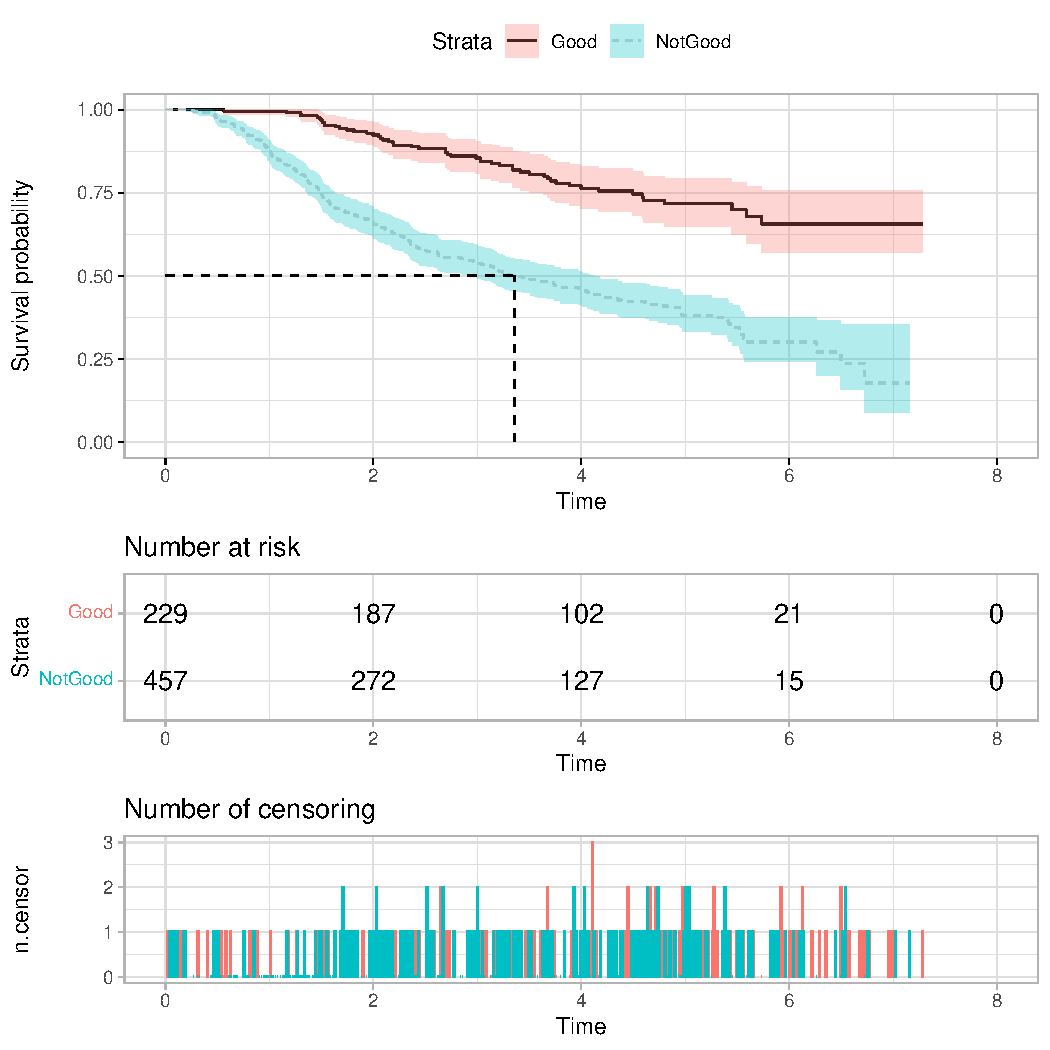
\includegraphics{C:/Users/g10028783/Downloads/R talks/PERSUADE//tests/testthat/grid_test/check_20_output/Images/Figure_plot_KM-1} \end{flushleft}

\begin{table}[H]
\centering
\caption{\label{tab:Table_1}Observed survival data}
\centering
\resizebox{\ifdim\width>\linewidth\linewidth\else\width\fi}{!}{
\begin{tabular}[t]{lrrrrrrrrr}
\toprule
  & records & n.max & n.start & events & rmean & se(rmean) & median & 0.95LCL & 0.95UCL\\
\midrule
\cellcolor{gray!10}{group=Good} & \cellcolor{gray!10}{229} & \cellcolor{gray!10}{229} & \cellcolor{gray!10}{229} & \cellcolor{gray!10}{51} & \cellcolor{gray!10}{5.934} & \cellcolor{gray!10}{0.1616} & \cellcolor{gray!10}{NA} & \cellcolor{gray!10}{NA} & \cellcolor{gray!10}{NA}\\
group=NotGood & 457 & 457 & 457 & 248 & 3.859 & 0.1349 & 3.356 & 2.959 & 4.115\\
\bottomrule
\end{tabular}}
\end{table}

\clearpage

\section{2. Proportional hazards
assumption}\label{proportional-hazards-assumption}

\textbf{Should stratified parametric survival models be used?}\\
To decide whether stratified or non-stratified parametric survival
models should be applied, it is important to assess whether the
\textbf{proportional hazards (PH) assumption} holds. This assumption
means that the hazard ratio between two (or more) groups remains
constant over time.

\begin{itemize}
\tightlist
\item
  \textbf{If the PH assumption holds:} Non-stratified parametric models
  can be used, with group effects included as covariates in a single
  model.\\
\item
  \textbf{If the PH assumption does not hold:} It is advised to fit
  separate (stratified) parametric survival models for each group.
\end{itemize}

This section presents plots for assessing the PH assumption \textbf{over
the observed data period only}. Even if the PH assumption appears valid
here, it might be violated beyond the observed follow-up. For further
details, see
\href{http://nicedsu.org.uk/wp-content/uploads/2016/03/NICE-DSU-TSD-Survival-analysis.updated-March-2013.v2.pdf}{NICE
DSU TSD 14}.

\textbf{How to interpret the figures:}

\begin{itemize}
\tightlist
\item
  \textbf{Figure A} plots the log of time against the log of the
  cumulative hazard for each group. Parallel lines suggest that the PH
  assumption holds.\\
\item
  \textbf{Figures B and C} show scaled Schoenfeld residuals over time,
  with a smoothed spline (cyan) overlaid. If the spline systematically
  deviates from a horizontal line, this suggests a time-varying
  covariate effect and a potential PH violation
  (\href{https://doi.org/10.1093/biomet/81.3.515}{Grambsch \& Therneau,
  1994}).\\
\item
  \textbf{Crossing survival curves} in the Kaplan--Meier plot (previous
  page) may also indicate that the PH assumption is not satisfied.
\end{itemize}

\textbf{Caution:} These diagnostics only apply to the observed data
period. Towards the end of follow-up, results may be unreliable due to
sparse data, so the tail of curves should be interpreted with care.

\clearpage

\begin{flushleft}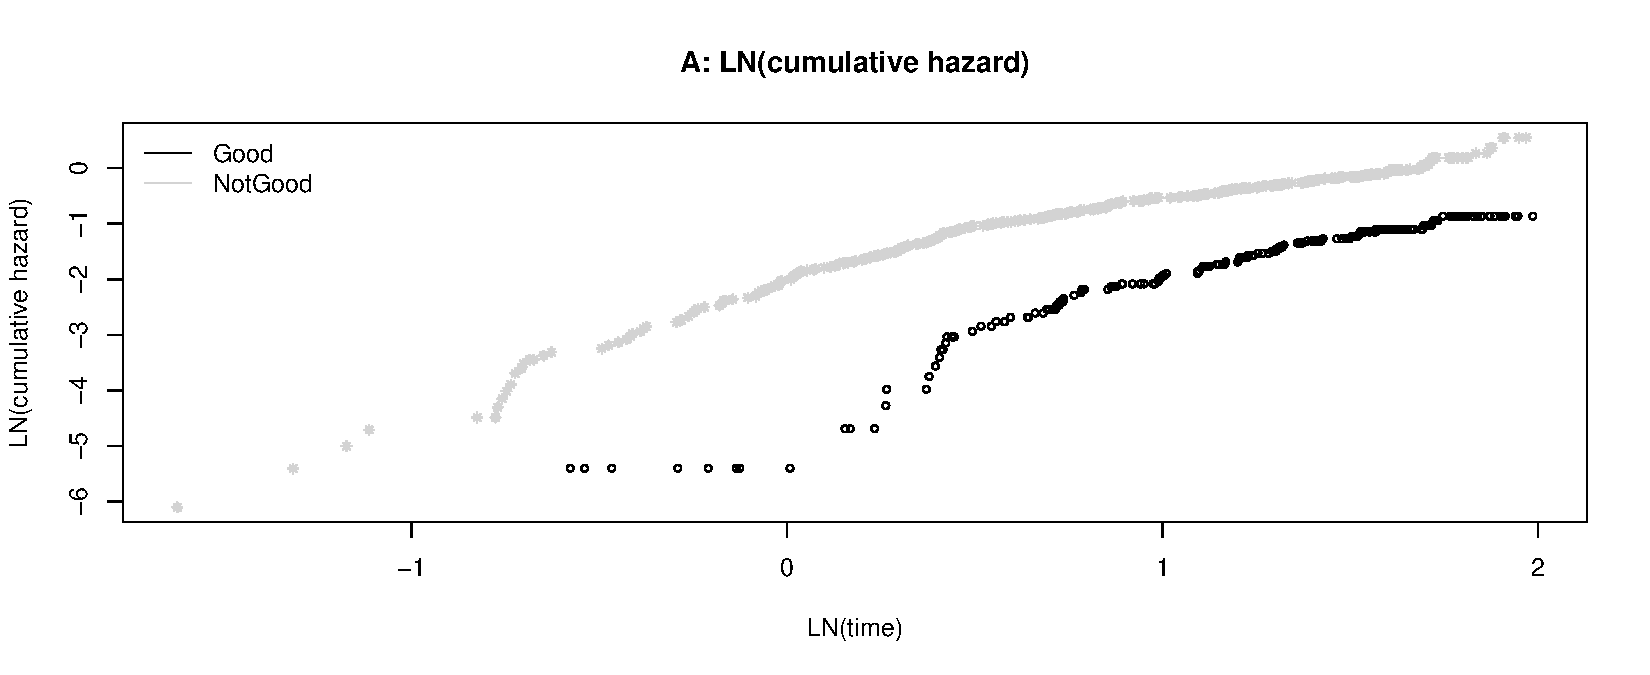
\includegraphics[height=0.29\textheight]{C:/Users/g10028783/Downloads/R talks/PERSUADE//tests/testthat/grid_test/check_20_output/Images/Figure_PH_assumption-1} \end{flushleft}

\begin{flushleft}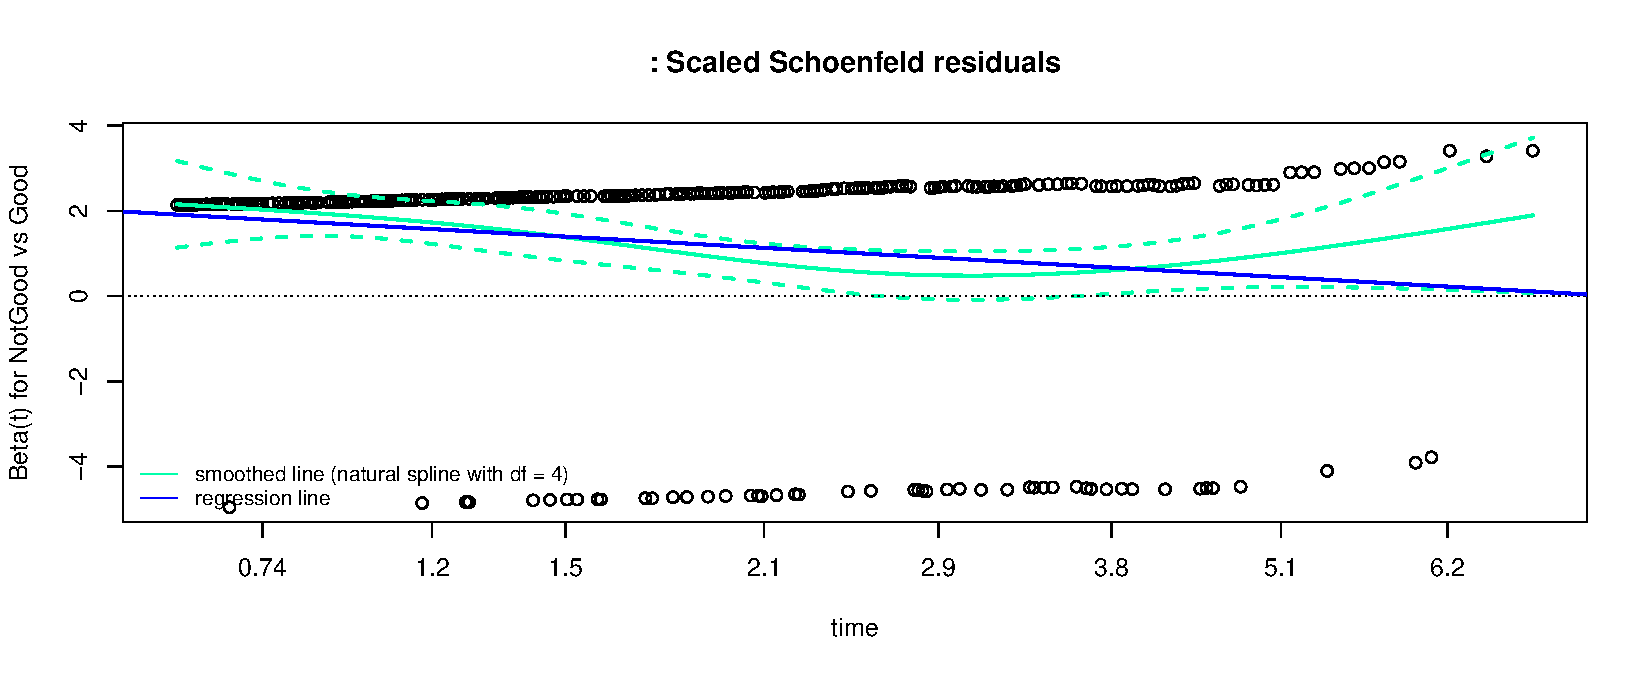
\includegraphics[height=0.29\textheight]{C:/Users/g10028783/Downloads/R talks/PERSUADE//tests/testthat/grid_test/check_20_output/Images/Figure_PH_assumption-2} \end{flushleft}

\clearpage

\section{3. Hazard function}\label{hazard-function}

\subsection{3.1 Shape of the observed smoothed hazard
function}\label{shape-of-the-observed-smoothed-hazard-function}

The \textbf{hazard function} represents the instantaneous rate at which
an event occurs at a specific time, conditional on survival until that
time. Its shape varies depending on the assumed distribution (parametric
survival model). When selecting an appropriate model, the plausibility
of different hazard function shapes should be considered in light of:

\begin{itemize}
\tightlist
\item
  The shape of the \emph{observed} hazard function (shown below).
\item
  Known hazard shapes from standard parametric models (see Table).
\item
  Relevant \emph{external data} (not shown here).
\end{itemize}

Below is an overview of the potential hazard shapes for standard
parametric survival models:

\begin{longtable}[]{@{}
  >{\raggedright\arraybackslash}p{(\columnwidth - 4\tabcolsep) * \real{0.0351}}
  >{\raggedright\arraybackslash}p{(\columnwidth - 4\tabcolsep) * \real{0.1930}}
  >{\raggedright\arraybackslash}p{(\columnwidth - 4\tabcolsep) * \real{0.7719}}@{}}
\toprule\noalign{}
\begin{minipage}[b]{\linewidth}\raggedright
No
\end{minipage} & \begin{minipage}[b]{\linewidth}\raggedright
Distribution
\end{minipage} & \begin{minipage}[b]{\linewidth}\raggedright
Hazard function shape
\end{minipage} \\
\midrule\noalign{}
\endhead
\bottomrule\noalign{}
\endlastfoot
1 & Exponential & Constant hazard \\
2 & Weibull & Monotonically increasing or decreasing hazards \\
3 & Gompertz & Monotonically increasing or decreasing hazards \\
4 & Log-normal & Arc-shaped or monotonically decreasing hazards \\
5 & Log-logistic & Arc-shaped or monotonically decreasing hazards \\
6 & Gamma & Monotonically increasing or decreasing hazards \\
7 & Generalised Gamma & Arc-shaped, bathtub-shaped, monotonically
increasing, or monotonically decreasing \\
\end{longtable}

Because \textbf{spline-based} and \textbf{(non-)mixture cure models} are
derived from these standard parametric forms, their hazard functions can
be interpreted in relation to the table above.

\begin{itemize}
\tightlist
\item
  For \textbf{spline-based models} using the \emph{hazard scale}, the
  baseline hazard is Weibull, so hazards are monotonic within each
  spline segment (between knots).\\
\item
  For \textbf{spline-based models} using the \emph{odds scale}
  (log-logistic) or \emph{normal scale} (log-normal), the baseline
  hazard follows the corresponding parametric form.\\
\item
  For \textbf{(non-)mixture cure models}, the hazard shape applies
  separately to the cure and non-cure fractions.
\end{itemize}

For more details and visualisations of hazard function shapes across
parametric survival models, see
\href{https://devinincerti.com/2019/06/18/parametric_survival.html}{Incerti
(2019)}.

\textbf{Caution:} These plots apply only to the \emph{observed} data
period and cannot directly inform the hazard shape beyond this range.
Additionally, hazard estimates near the end of follow-up may be unstable
due to sparse data. Interpret the tails of the curves with care.

\clearpage

\begin{flushleft}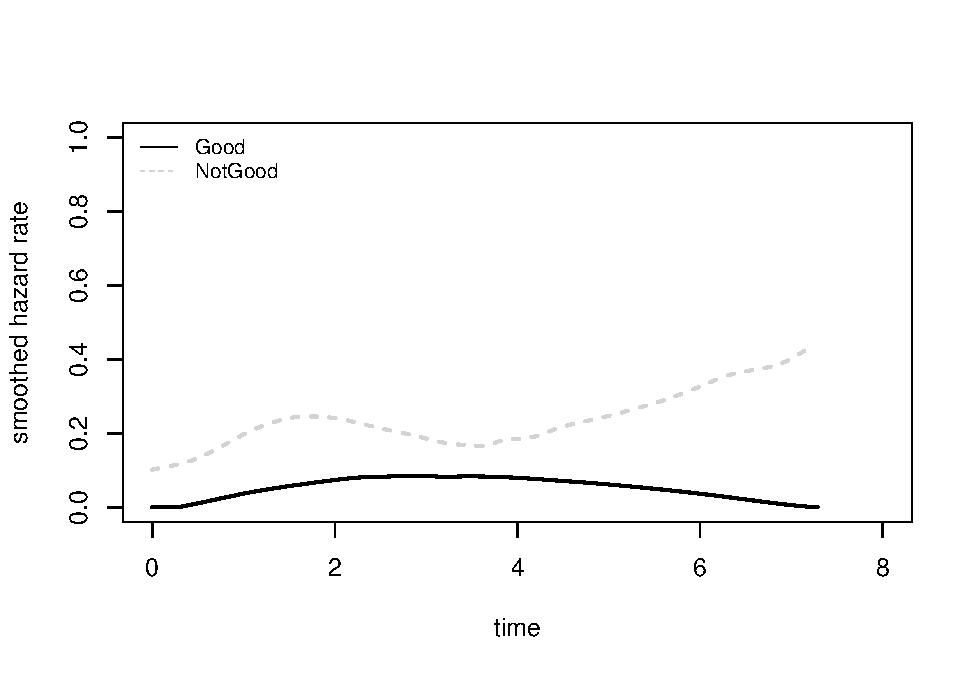
\includegraphics{C:/Users/g10028783/Downloads/R talks/PERSUADE//tests/testthat/grid_test/check_20_output/Images/Figure_plot_hr-1} \end{flushleft}

\clearpage

\subsection{3.2 Shape of the predicted hazard
function}\label{shape-of-the-predicted-hazard-function}

The following plots show how the hazard rate is estimated under each
fitted parametric survival model. These curves reflect the model-based
\emph{predicted} hazard functions over time, which may extend beyond the
observed data period (see \emph{Extrapolation Section}). By comparing
these predicted hazard shapes, together with the known hazard function
form for each parametric model, to:

\begin{itemize}
\tightlist
\item
  The \textbf{observed smoothed hazard functions}, and\\
\item
  Prior knowledge or external evidence on plausible hazard behaviour,
\end{itemize}

you can assess whether each model's functional form provides a
reasonable representation and extrapolation of the underlying event
process.

\clearpage

\begin{flushleft}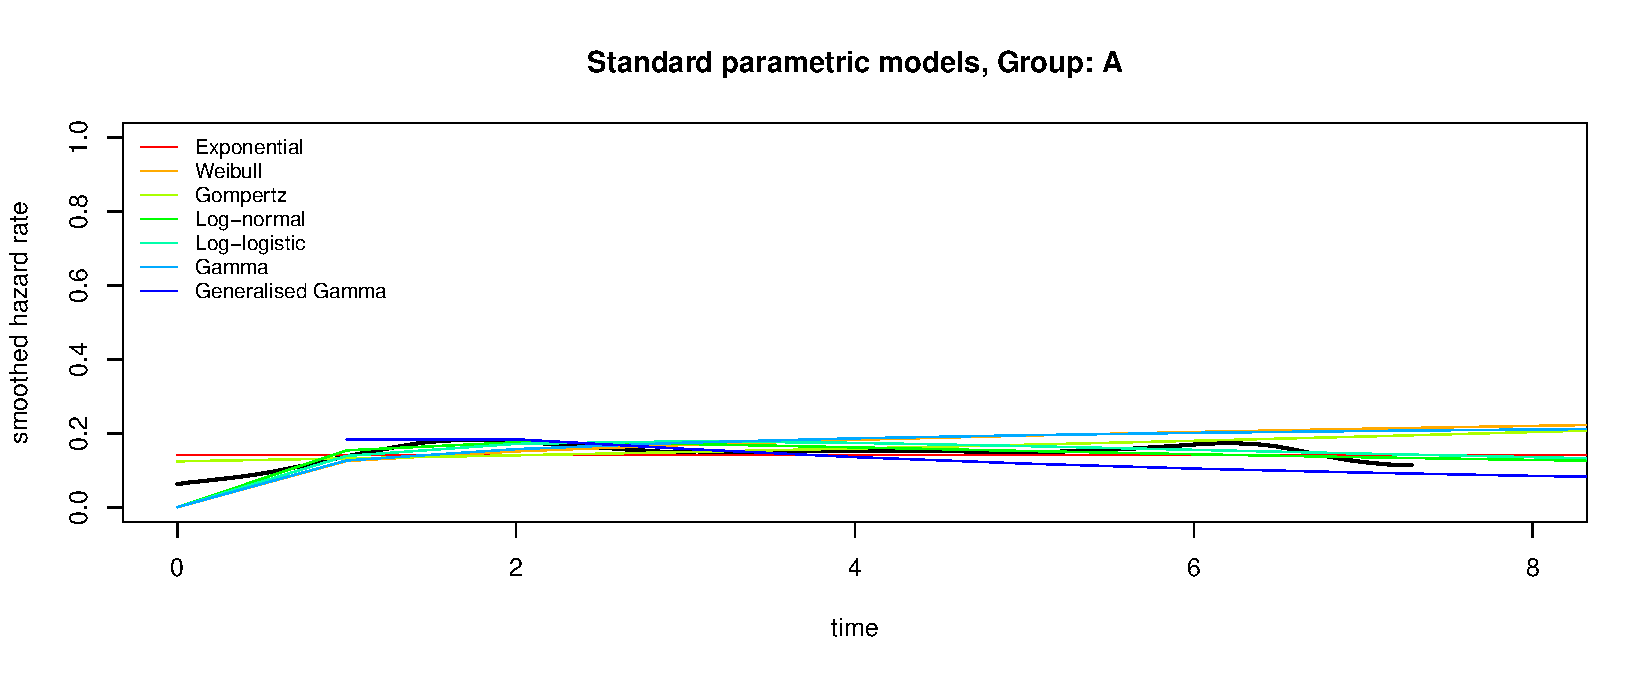
\includegraphics[height=0.29\textheight]{C:/Users/g10028783/Downloads/R talks/PERSUADE//tests/testthat/grid_test/check_20_output/Images/Figure_plot_haz_pred-1} \end{flushleft}

\begin{flushleft}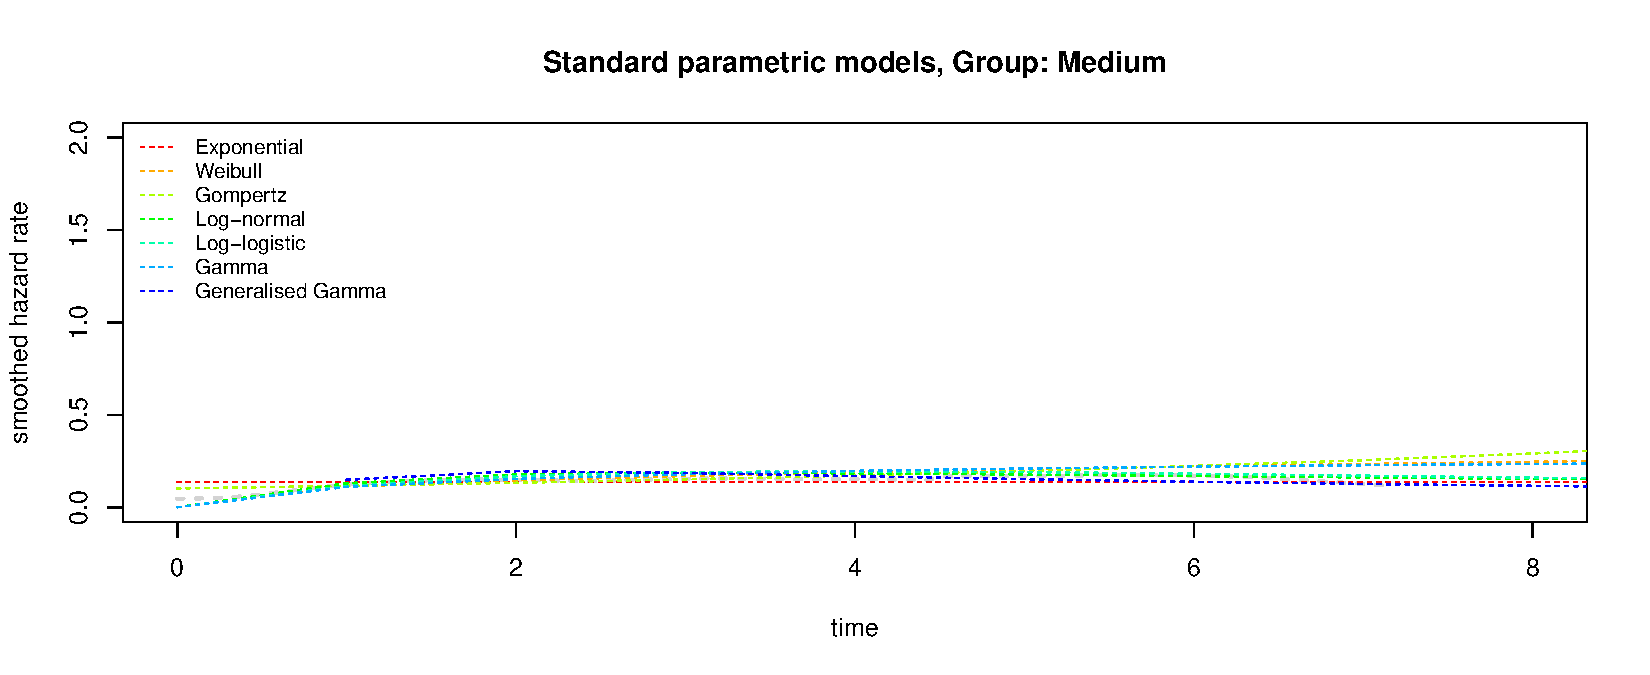
\includegraphics[height=0.29\textheight]{C:/Users/g10028783/Downloads/R talks/PERSUADE//tests/testthat/grid_test/check_20_output/Images/Figure_plot_haz_pred-2} \end{flushleft}

\begin{flushleft}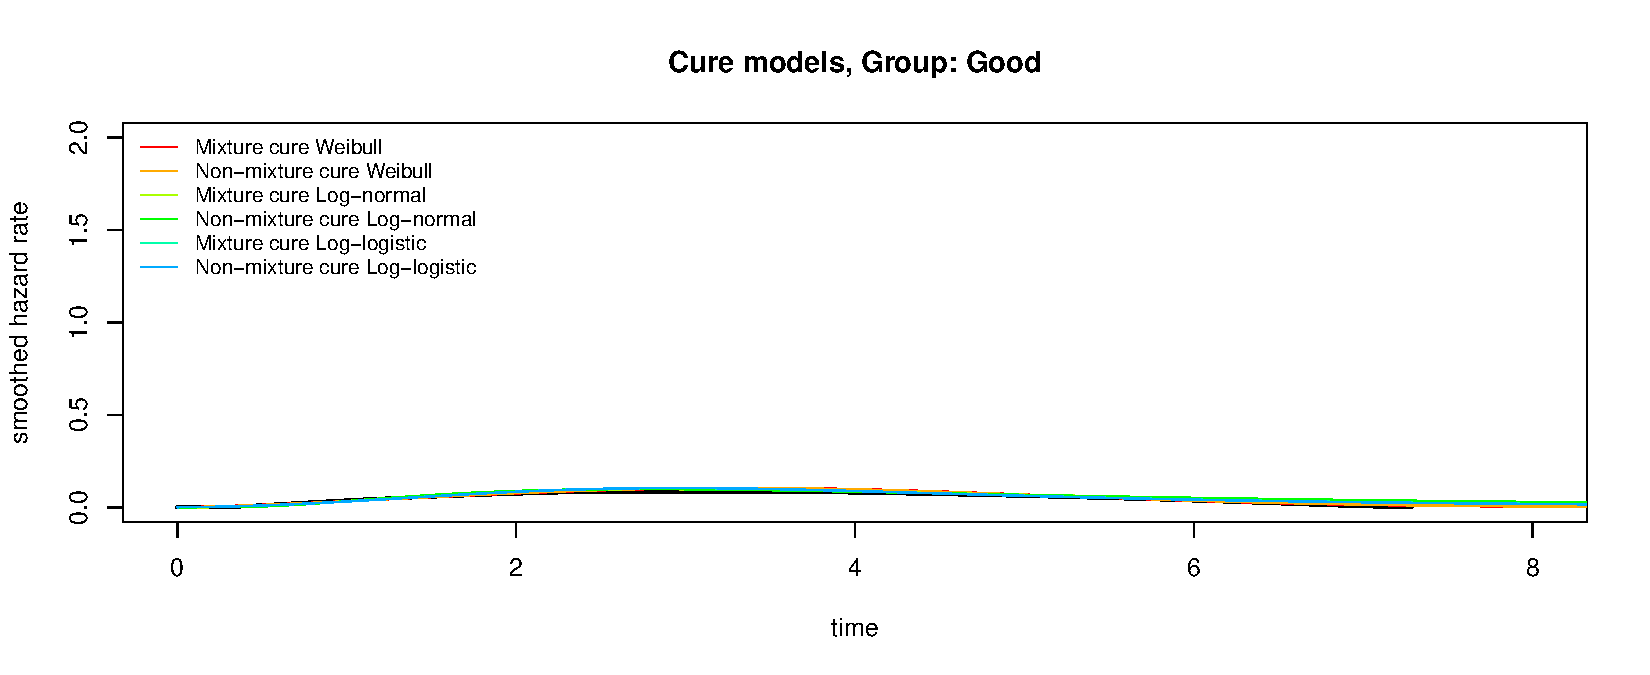
\includegraphics[height=0.29\textheight]{C:/Users/g10028783/Downloads/R talks/PERSUADE//tests/testthat/grid_test/check_20_output/Images/Figure_plot_haz_pred-3} \end{flushleft}

\begin{flushleft}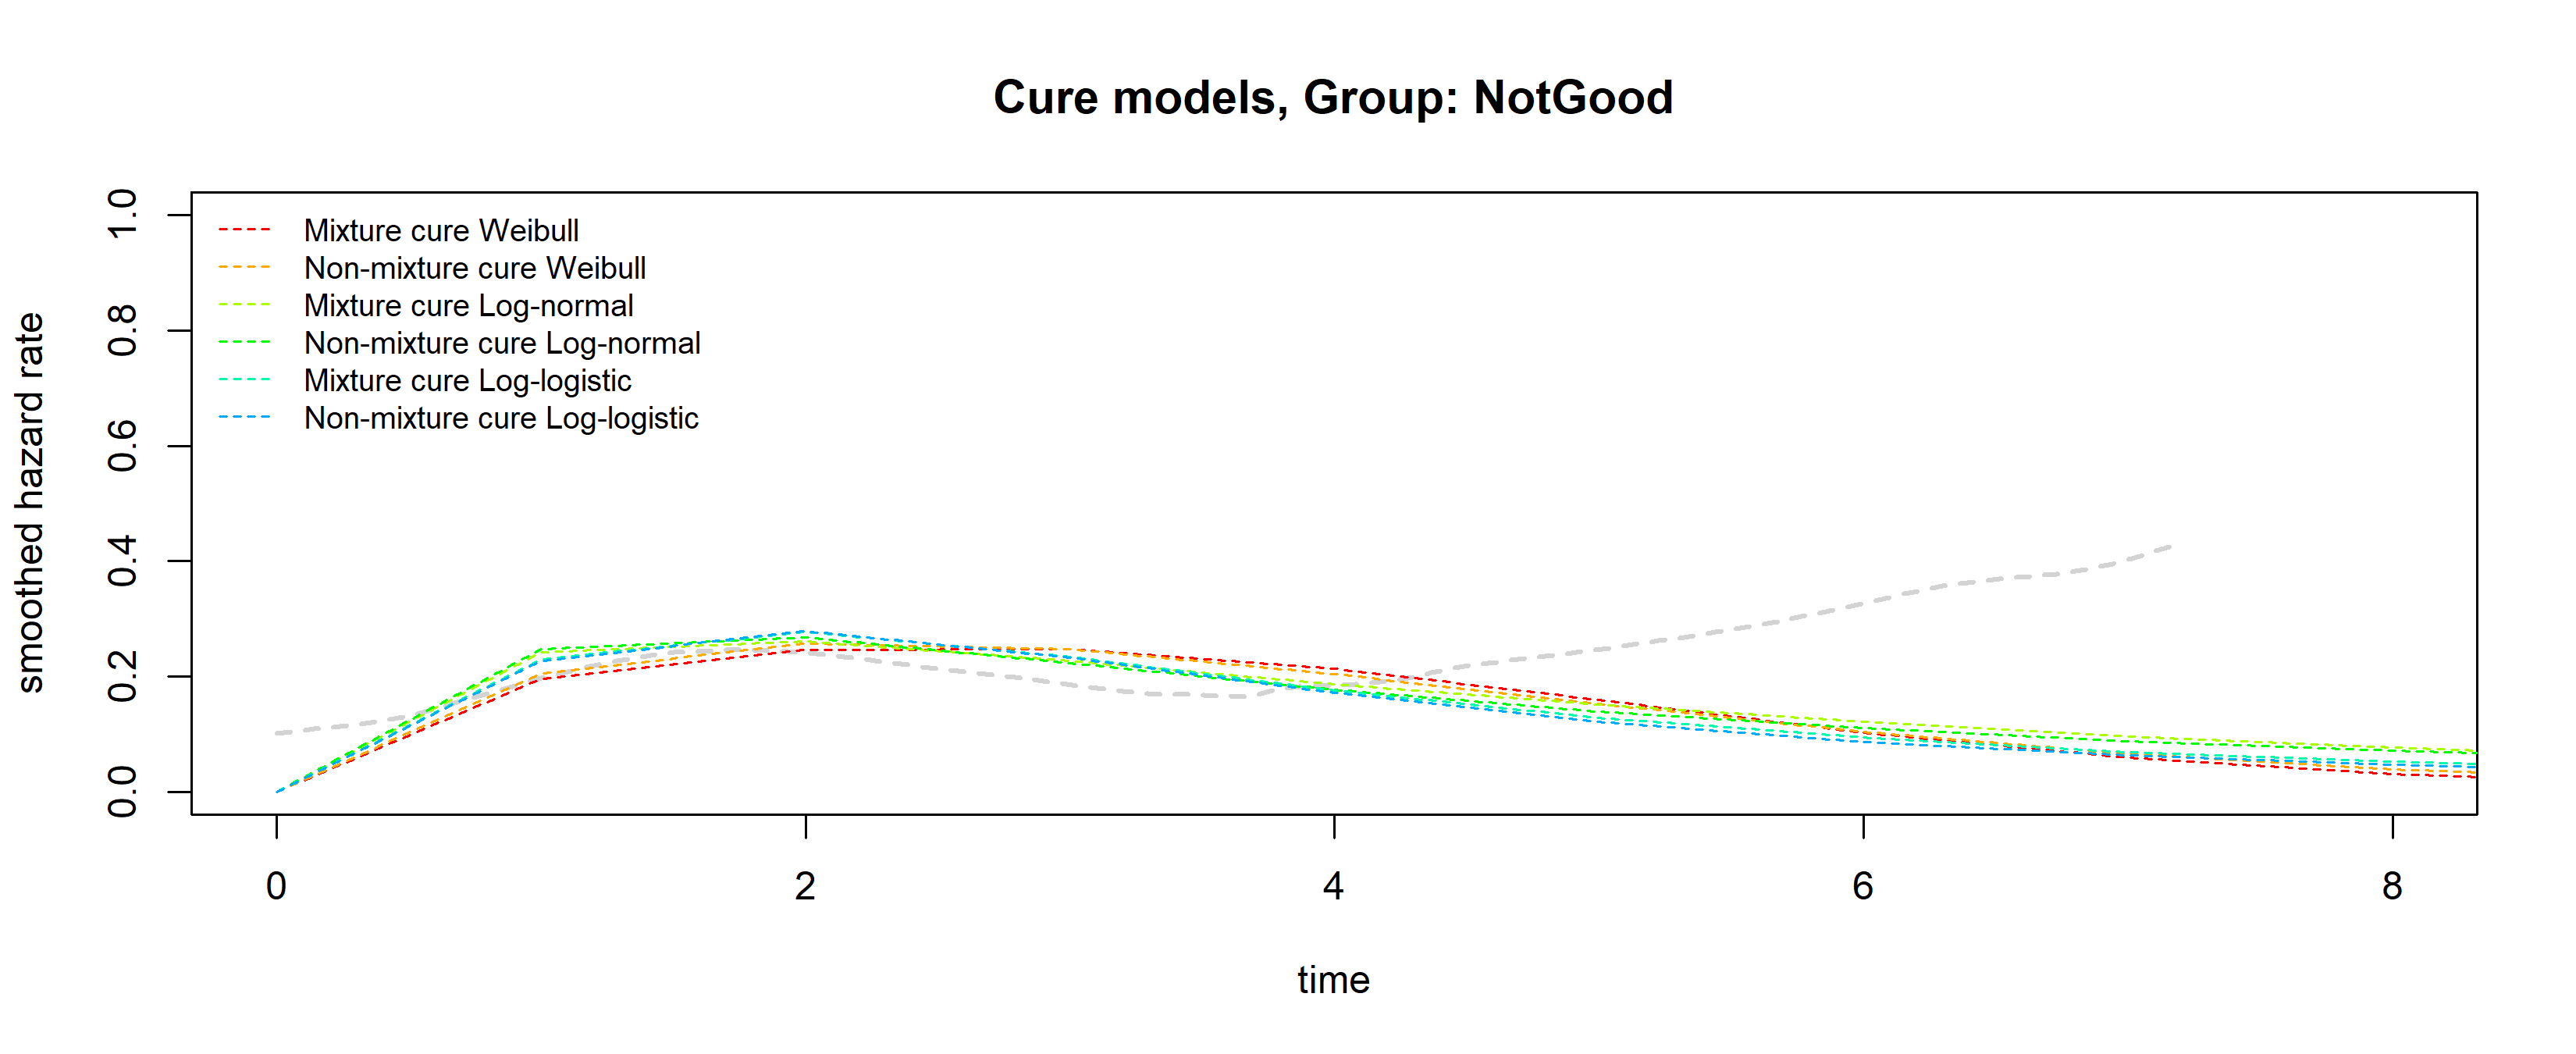
\includegraphics[height=0.29\textheight]{C:/Users/g10028783/Downloads/R talks/PERSUADE//tests/testthat/grid_test/check_20_output/Images/Figure_plot_haz_pred-4} \end{flushleft}

\clearpage

\section{4 Parametric survival models}\label{parametric-survival-models}

\subsection{4.1 Standard parametric
models}\label{standard-parametric-models}

The Table below displays the goodness-of-fit statistics for each
parametric survival model, ordered from `best' fitting to less well
fitting based on the Akaike Information Criterion (AIC). The AIC and
Bayesian Information Criterion (BIC) provide a measure of the relative
fit of each model to the observed data, while penalising for the number
of parameters included in the fitted models. The lower the AIC or BIC,
the better the relative fit of a model compared to other fitted models.

\textbf{Rules of thumb for model selection}:

\begin{itemize}
\tightlist
\item
  \textbf{Burnham and Anderson} (1998) suggest that models with an AIC
  within 4 points of the lowest AIC can be considered as having
  substantial support from the data
  \href{https://doi.org/10.1007/978-1-4757-2917-7}{Burnham and Anderson,
  1998}.\\
\item
  \textbf{Raftery} (1995) suggests that models with a BIC within 2
  points of the lowest BIC can be considered the best-fitting models
  \href{https://doi.org/10.2307/271063}{Raftery et al., 1995}.
\end{itemize}

In the following pages, three plots per fitted parametric survival model
are displayed to support visual inspection of the fit of the models to
the observed data:

\begin{itemize}
\tightlist
\item
  \textbf{Figure A}: Kaplan--Meier curves (black and grey) versus fitted
  parametric survival models (colour).\\
\item
  \textbf{Figure B}: Diagnostic plot specific to each fitted parametric
  survival model (see graphical test in Table 1 of
  \href{https://doi.org/10.1007/s40273-013-0064-3}{Ishak et al., 2013}).
\item
  \textbf{Figure C}: Comparison of smoothed hazard rates based on
  empirical data (black and grey) versus estimated transition
  probabilities (colour).
\end{itemize}

In Figures A and C, the Kaplan--Meier curves and smoothed hazard rates
are identical across models; only the coloured fitted curves change.\\
The guiding rule is: the closer the coloured lines are to the black and
grey lines, the better the fit.

Notably:

\begin{itemize}
\tightlist
\item
  Weibull (shape = 1), Gompertz (shape = 0) and gamma (shape = 1)
  distributions simplify to the exponential distribution.\\
\item
  The generalised gamma distribution simplifies to: -- Log-normal (Q =
  0)\\
  -- Weibull (Q = 1)\\
  -- Exponential (Q = 1 and scale = 1)\\
  -- Gamma (Q = scale)
\end{itemize}

Information regarding parameterisation of parametric survival models can
be found
\href{https://devinincerti.com/code/survival-distributions.html}{here}.

\textbf{CAUTION}:\\
These goodness-of-fit statistics apply only to the \emph{observed} data
period. They do not indicate the suitability of extrapolated survival
beyond this period. Additionally, the tail of the observed data period
may be affected by a low number of observations, which should be
considered when interpreting model performance.

\clearpage

\begin{table}[H]
\centering
\caption{\label{tab:Table_2}Goodness of fit statistics}
\centering
\resizebox{\ifdim\width>\linewidth\linewidth\else\width\fi}{!}{
\begin{tabular}[t]{lrr}
\toprule
Model & AIC & BIC\\
\midrule
\cellcolor{gray!10}{Generalised Gamma} & \cellcolor{gray!10}{1619} & \cellcolor{gray!10}{1637}\\
Log-normal & 1627 & 1640\\
\cellcolor{gray!10}{Log-logistic} & \cellcolor{gray!10}{1646} & \cellcolor{gray!10}{1659}\\
Gamma & 1660 & 1674\\
\cellcolor{gray!10}{Weibull} & \cellcolor{gray!10}{1671} & \cellcolor{gray!10}{1685}\\
Gompertz & 1694 & 1707\\
\cellcolor{gray!10}{Exponential} & \cellcolor{gray!10}{1698} & \cellcolor{gray!10}{1707}\\
\bottomrule
\end{tabular}}
\end{table}

\clearpage

\clearpage

\subsubsection{Exponential}\label{exponential}

\begin{flushleft}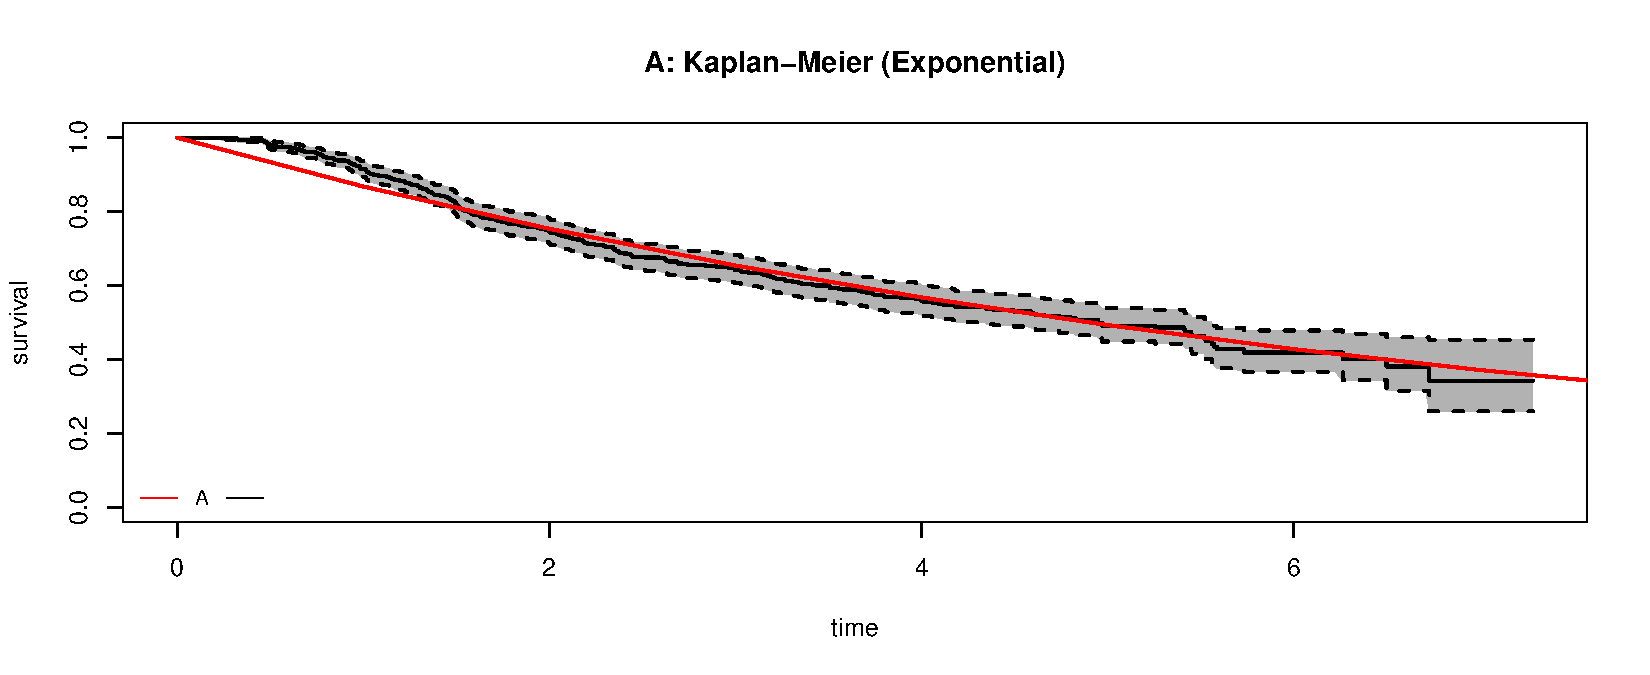
\includegraphics[height=0.25\textheight]{C:/Users/g10028783/Downloads/R talks/PERSUADE//tests/testthat/grid_test/check_20_output/Images/Figure_param_models-1} \end{flushleft}

\begin{flushleft}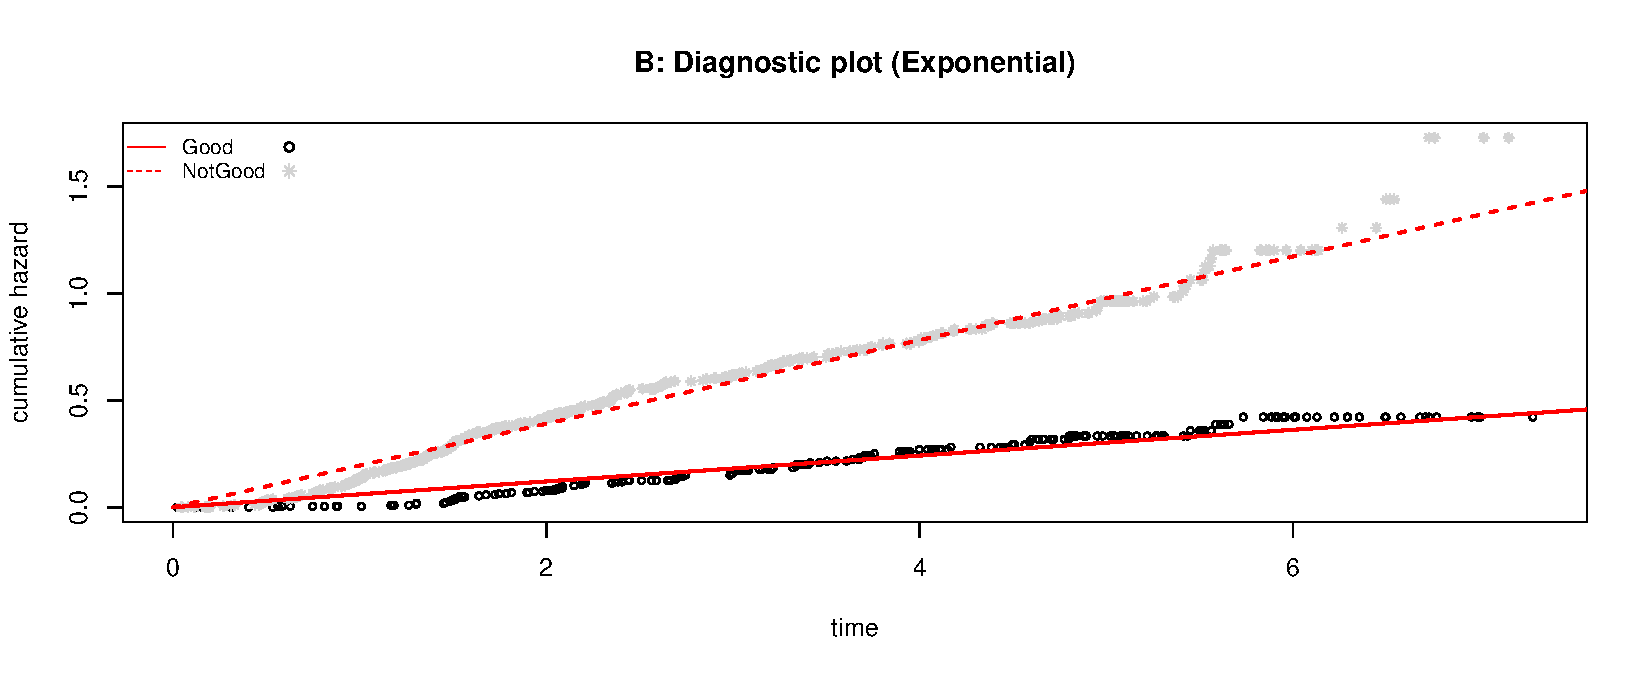
\includegraphics[height=0.25\textheight]{C:/Users/g10028783/Downloads/R talks/PERSUADE//tests/testthat/grid_test/check_20_output/Images/Figure_param_models-2} \end{flushleft}

\begin{flushleft}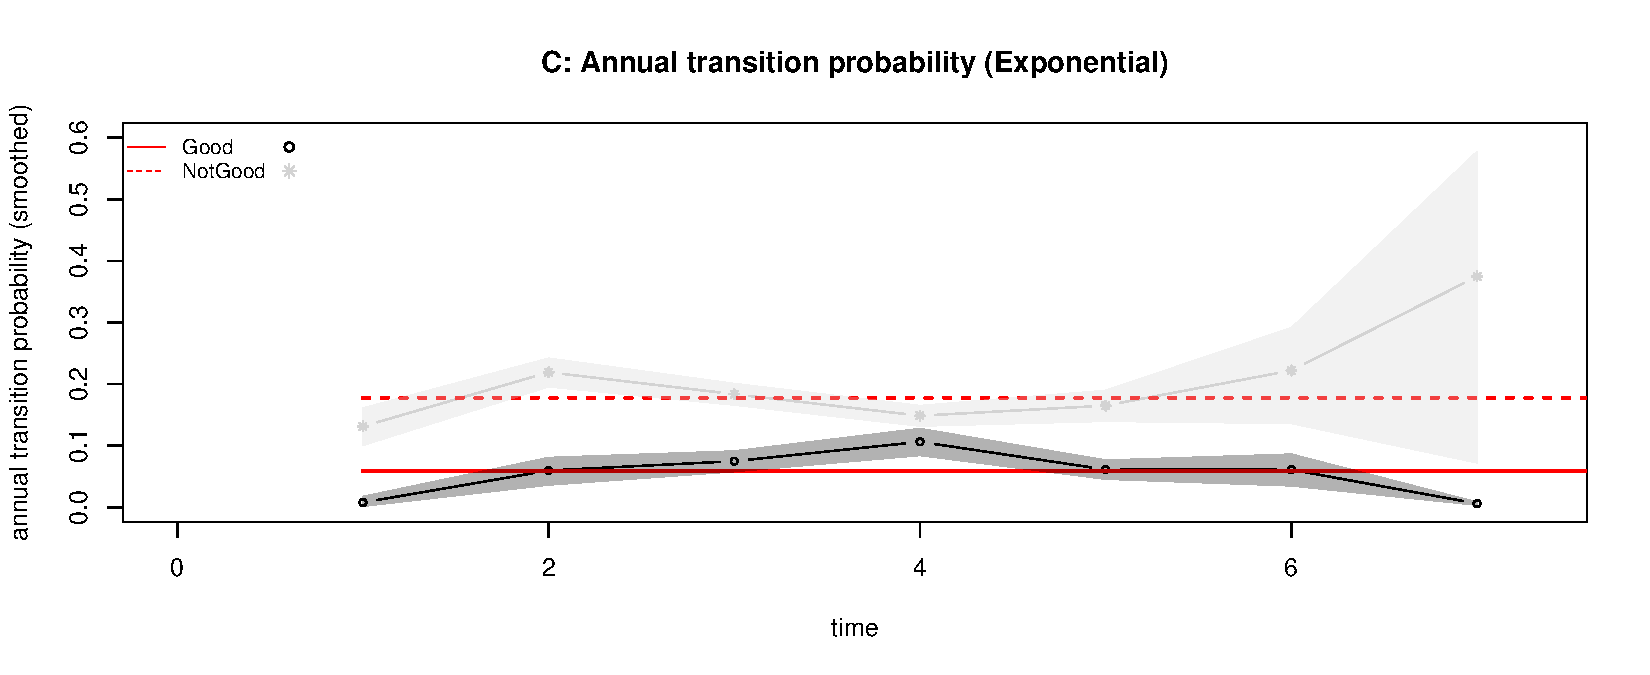
\includegraphics[height=0.25\textheight]{C:/Users/g10028783/Downloads/R talks/PERSUADE//tests/testthat/grid_test/check_20_output/Images/Figure_param_models-3} \end{flushleft}

\clearpage

\subsubsection{Weibull}\label{weibull}

\begin{flushleft}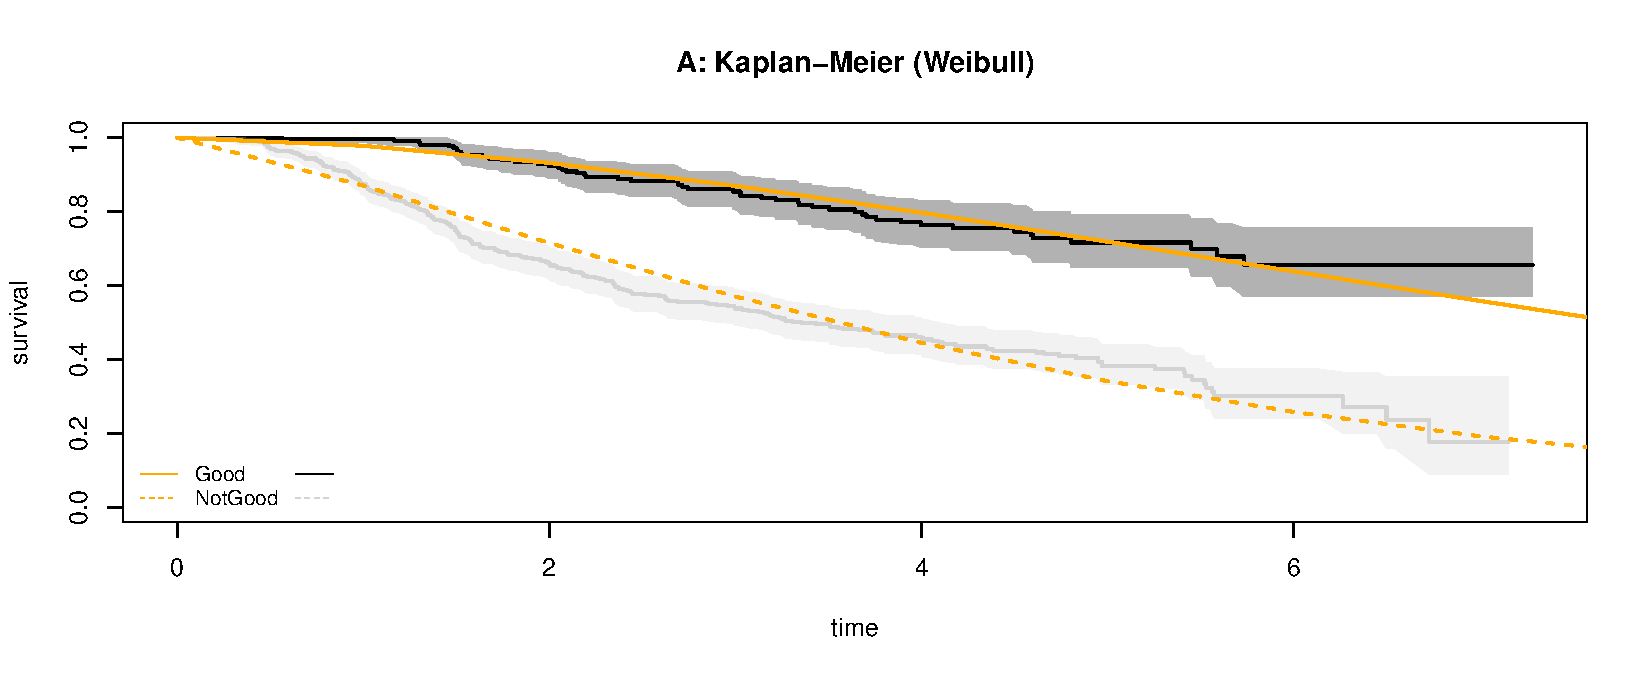
\includegraphics[height=0.25\textheight]{C:/Users/g10028783/Downloads/R talks/PERSUADE//tests/testthat/grid_test/check_20_output/Images/Figure_param_models-4} \end{flushleft}

\begin{flushleft}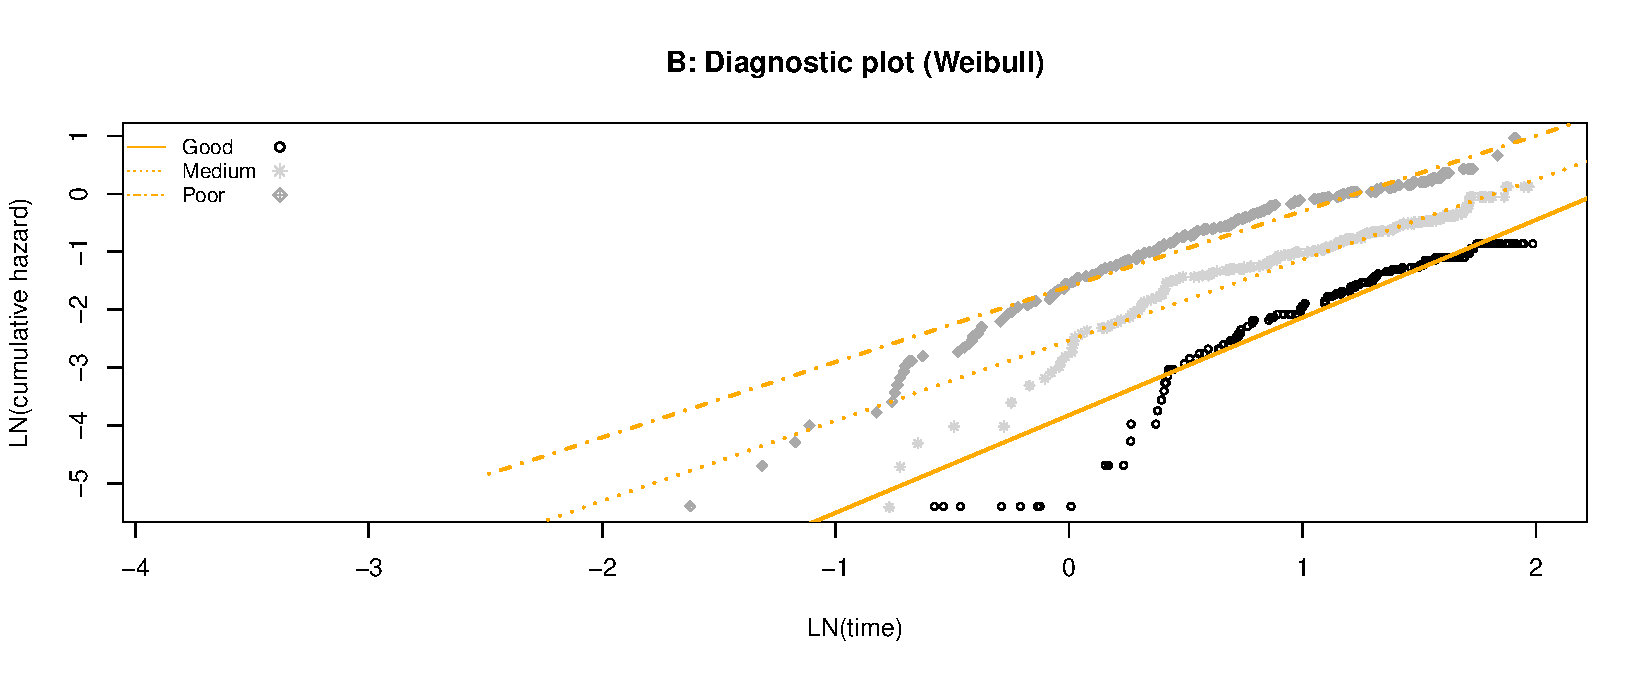
\includegraphics[height=0.25\textheight]{C:/Users/g10028783/Downloads/R talks/PERSUADE//tests/testthat/grid_test/check_20_output/Images/Figure_param_models-5} \end{flushleft}

\begin{flushleft}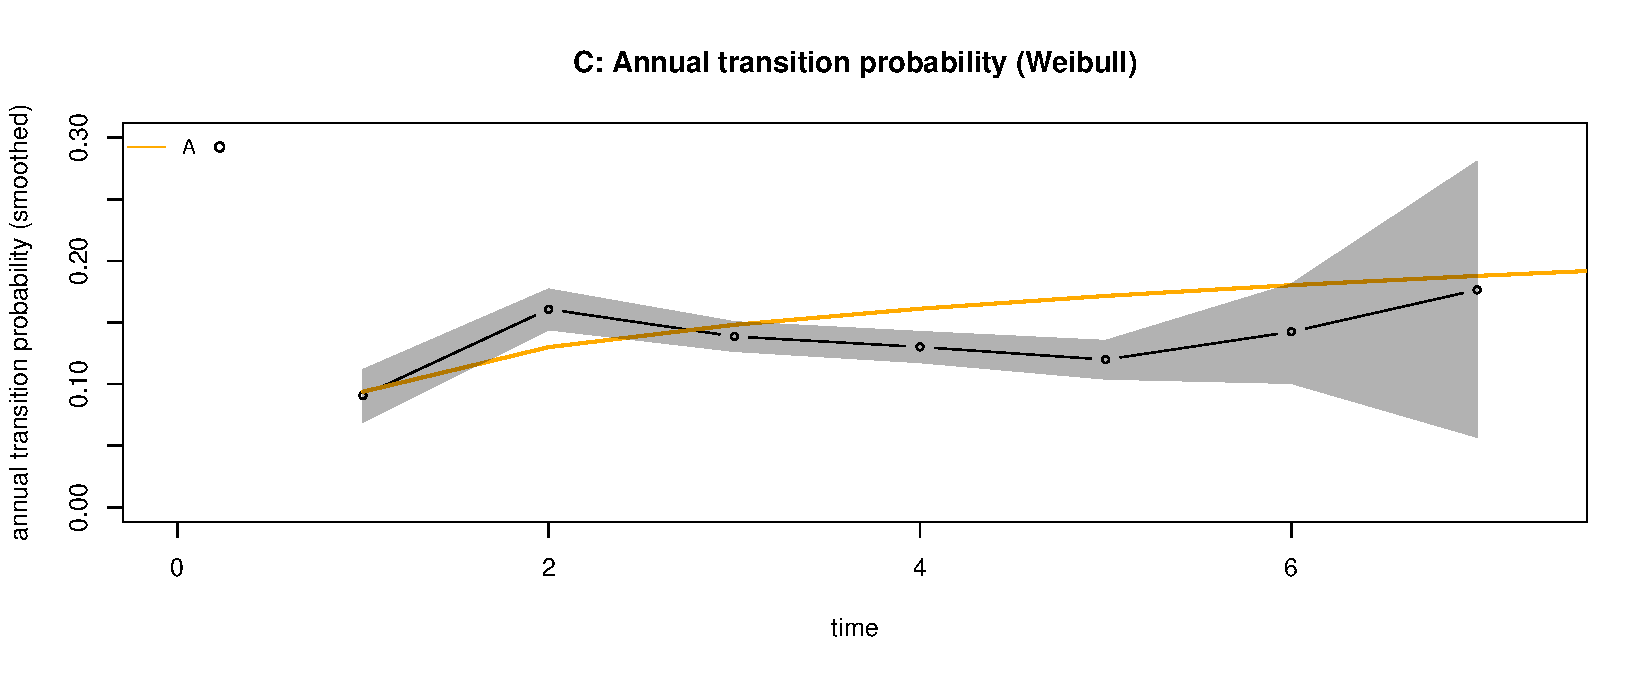
\includegraphics[height=0.25\textheight]{C:/Users/g10028783/Downloads/R talks/PERSUADE//tests/testthat/grid_test/check_20_output/Images/Figure_param_models-6} \end{flushleft}

\clearpage

\subsubsection{Gompertz}\label{gompertz}

\begin{flushleft}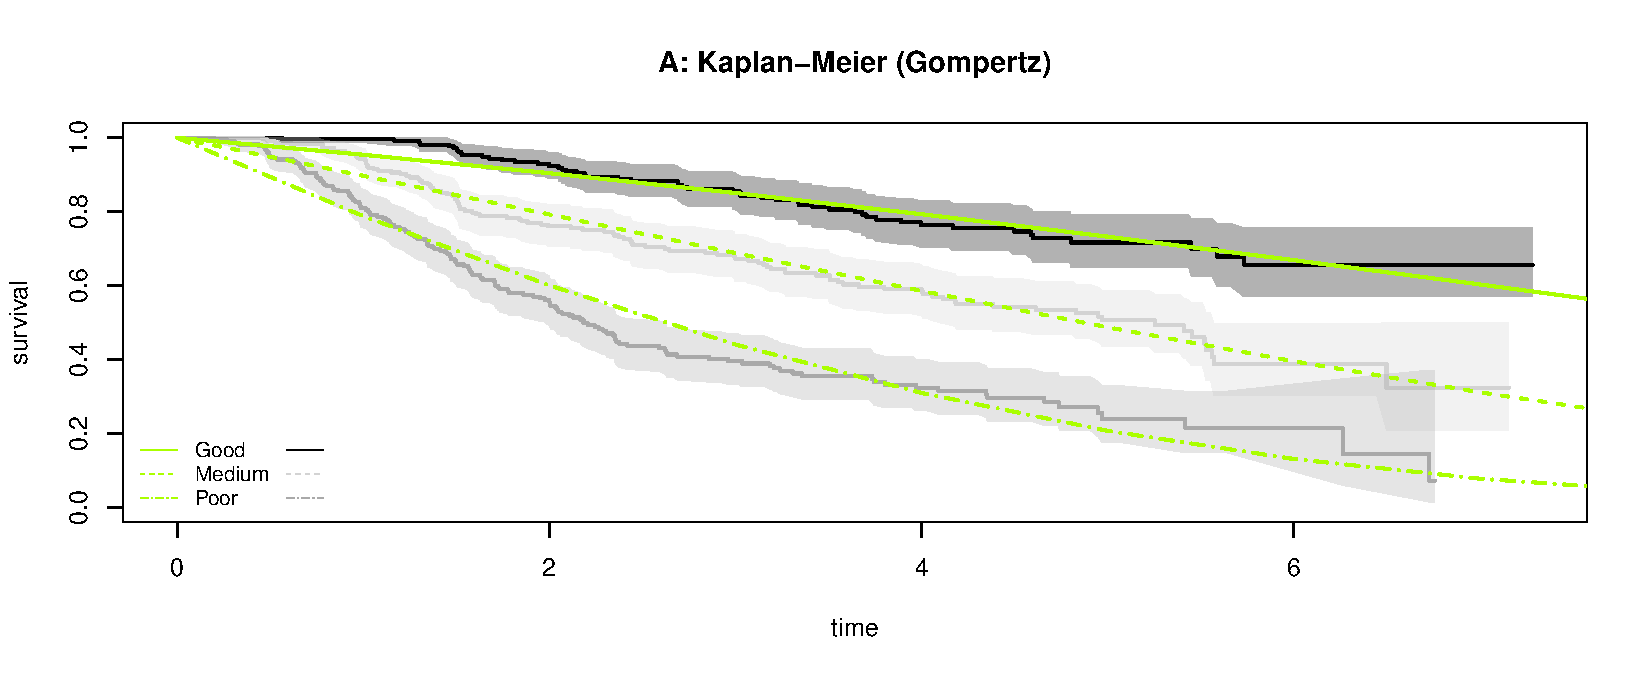
\includegraphics[height=0.25\textheight]{C:/Users/g10028783/Downloads/R talks/PERSUADE//tests/testthat/grid_test/check_20_output/Images/Figure_param_models-7} \end{flushleft}

\begin{flushleft}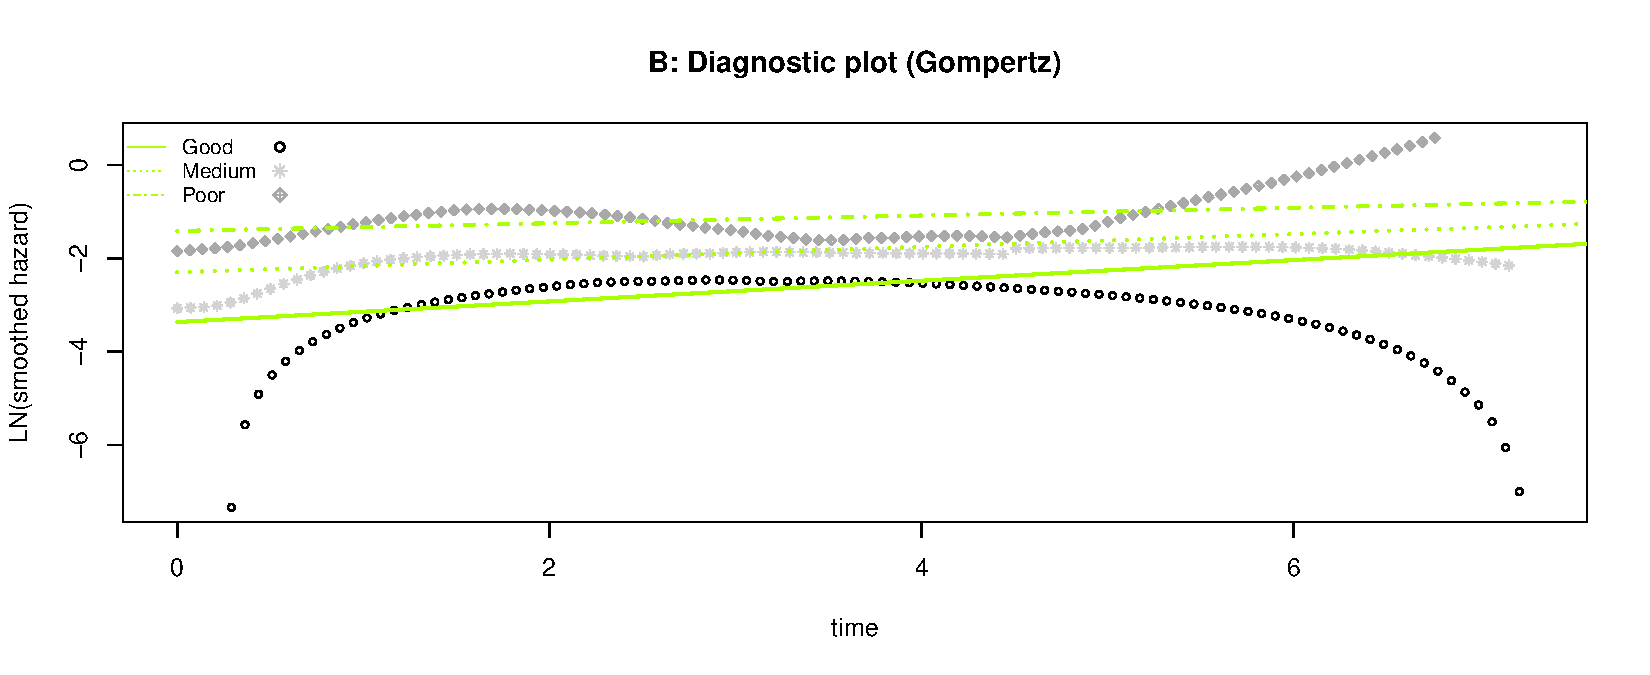
\includegraphics[height=0.25\textheight]{C:/Users/g10028783/Downloads/R talks/PERSUADE//tests/testthat/grid_test/check_20_output/Images/Figure_param_models-8} \end{flushleft}

\begin{flushleft}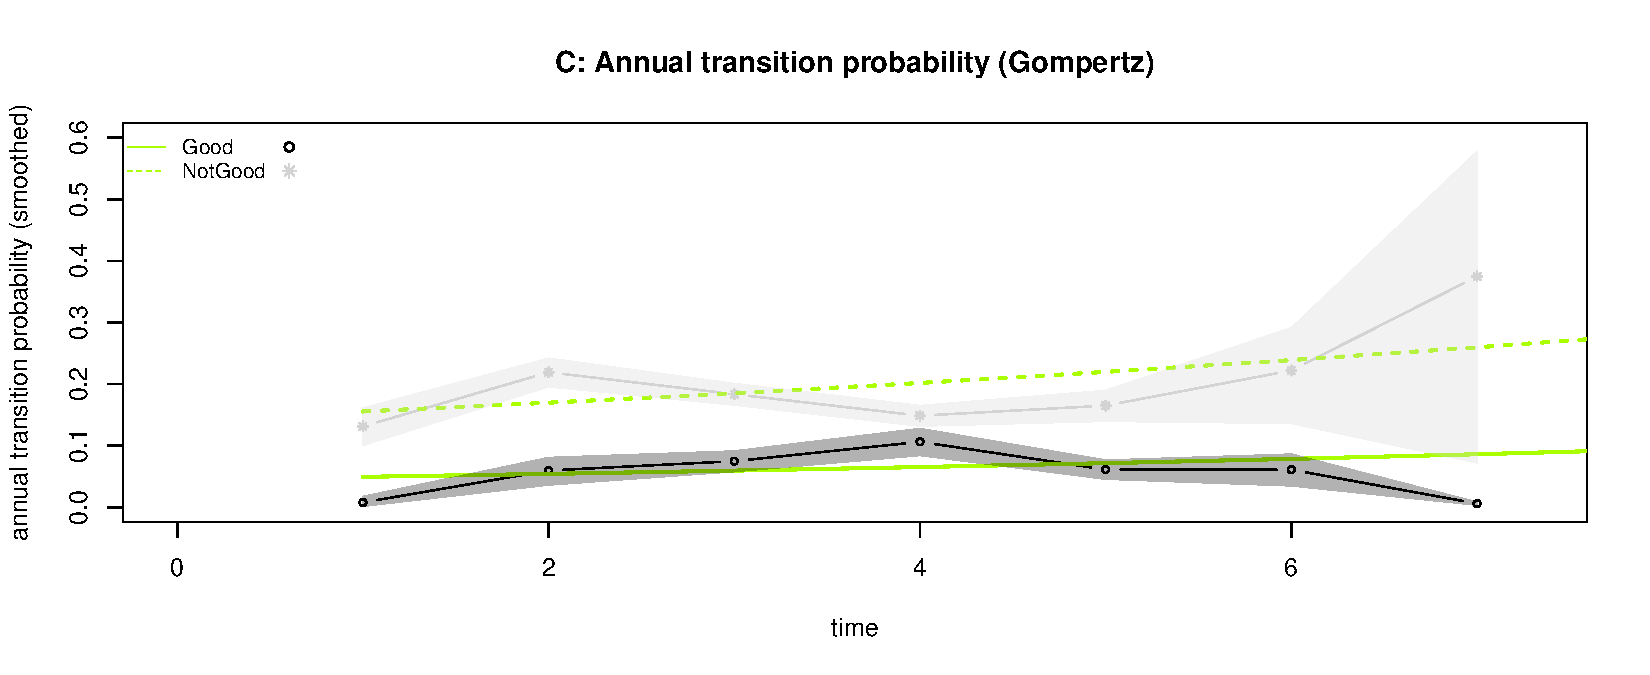
\includegraphics[height=0.25\textheight]{C:/Users/g10028783/Downloads/R talks/PERSUADE//tests/testthat/grid_test/check_20_output/Images/Figure_param_models-9} \end{flushleft}

\clearpage

\subsubsection{Log-normal}\label{log-normal}

\begin{flushleft}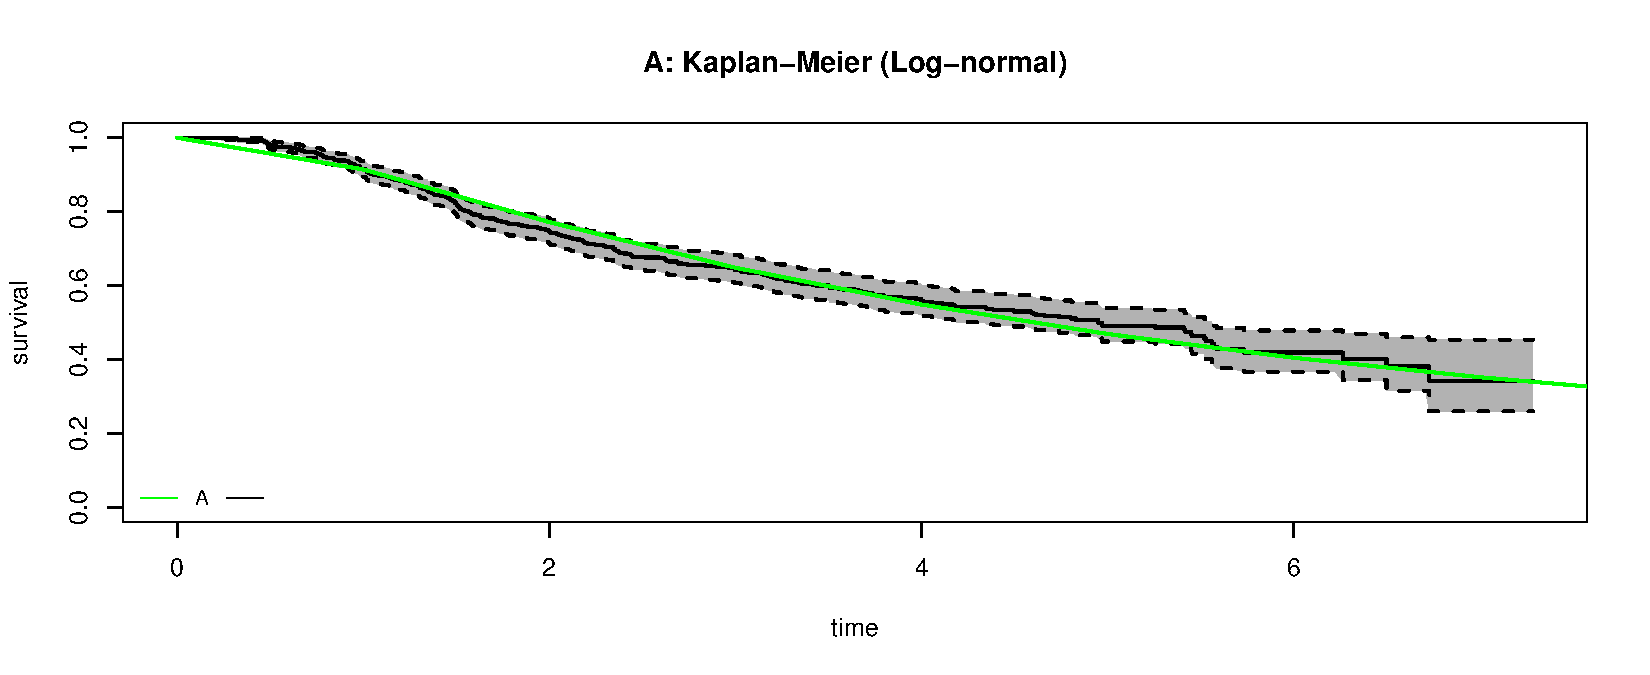
\includegraphics[height=0.25\textheight]{C:/Users/g10028783/Downloads/R talks/PERSUADE//tests/testthat/grid_test/check_20_output/Images/Figure_param_models-10} \end{flushleft}

\begin{flushleft}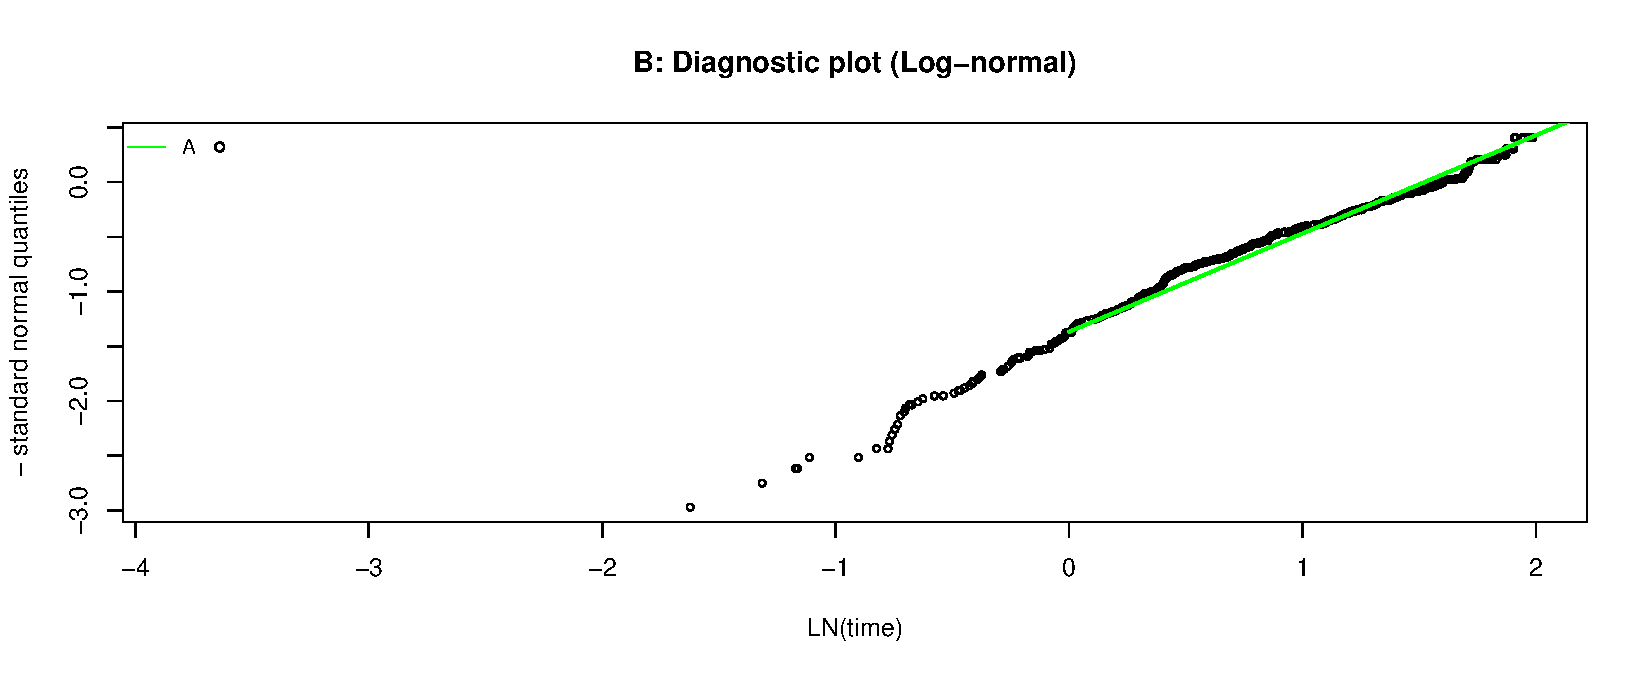
\includegraphics[height=0.25\textheight]{C:/Users/g10028783/Downloads/R talks/PERSUADE//tests/testthat/grid_test/check_20_output/Images/Figure_param_models-11} \end{flushleft}

\begin{flushleft}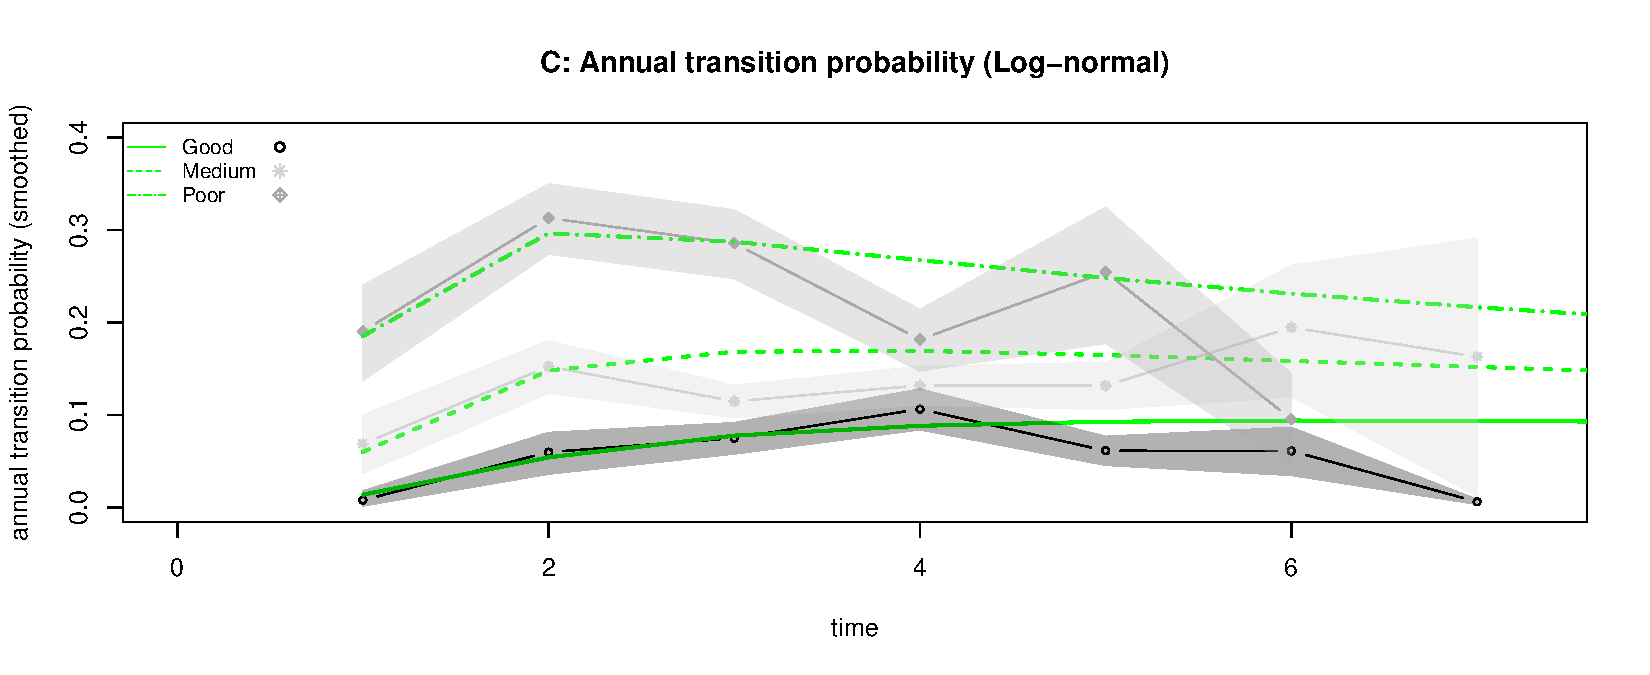
\includegraphics[height=0.25\textheight]{C:/Users/g10028783/Downloads/R talks/PERSUADE//tests/testthat/grid_test/check_20_output/Images/Figure_param_models-12} \end{flushleft}

\clearpage

\subsubsection{Log-logistic}\label{log-logistic}

\begin{flushleft}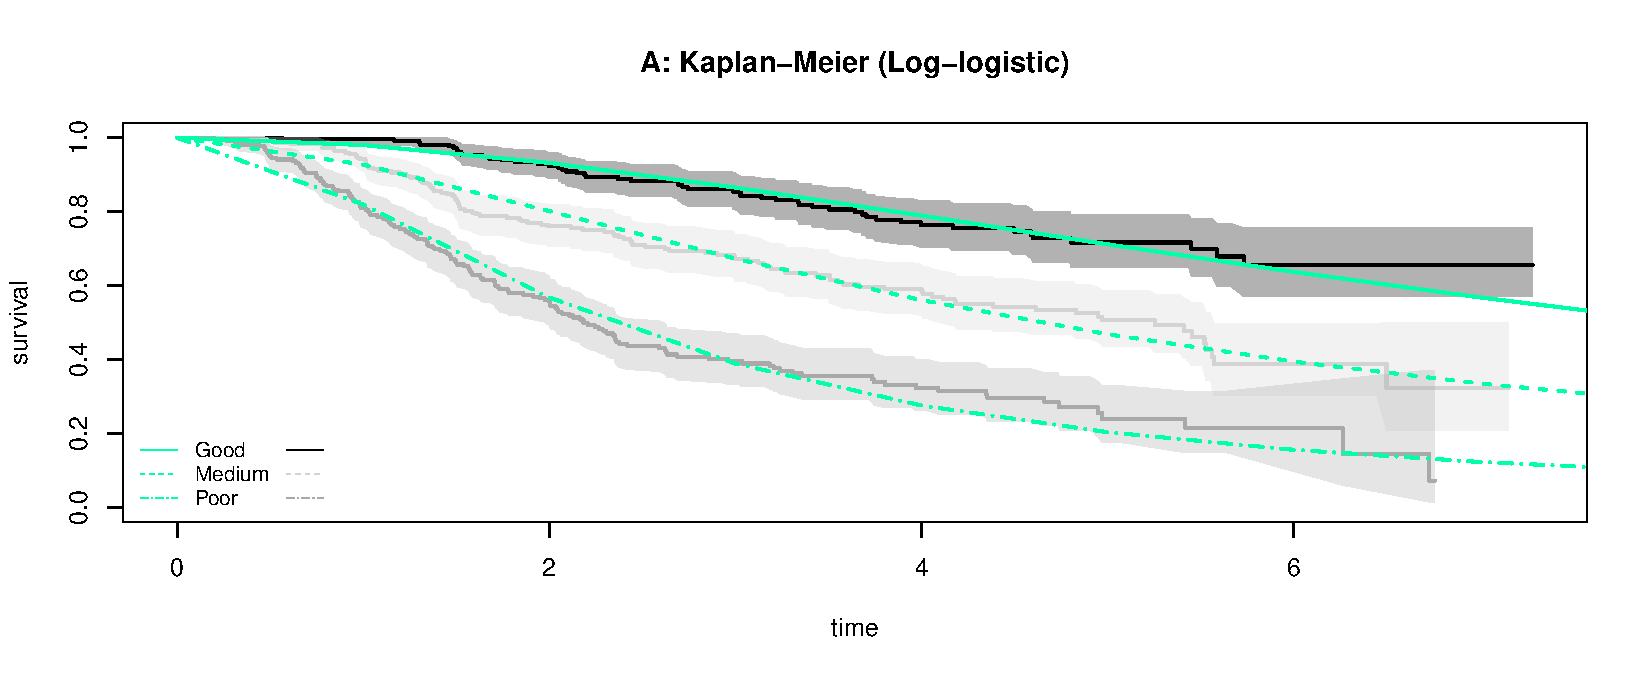
\includegraphics[height=0.25\textheight]{C:/Users/g10028783/Downloads/R talks/PERSUADE//tests/testthat/grid_test/check_20_output/Images/Figure_param_models-13} \end{flushleft}

\begin{flushleft}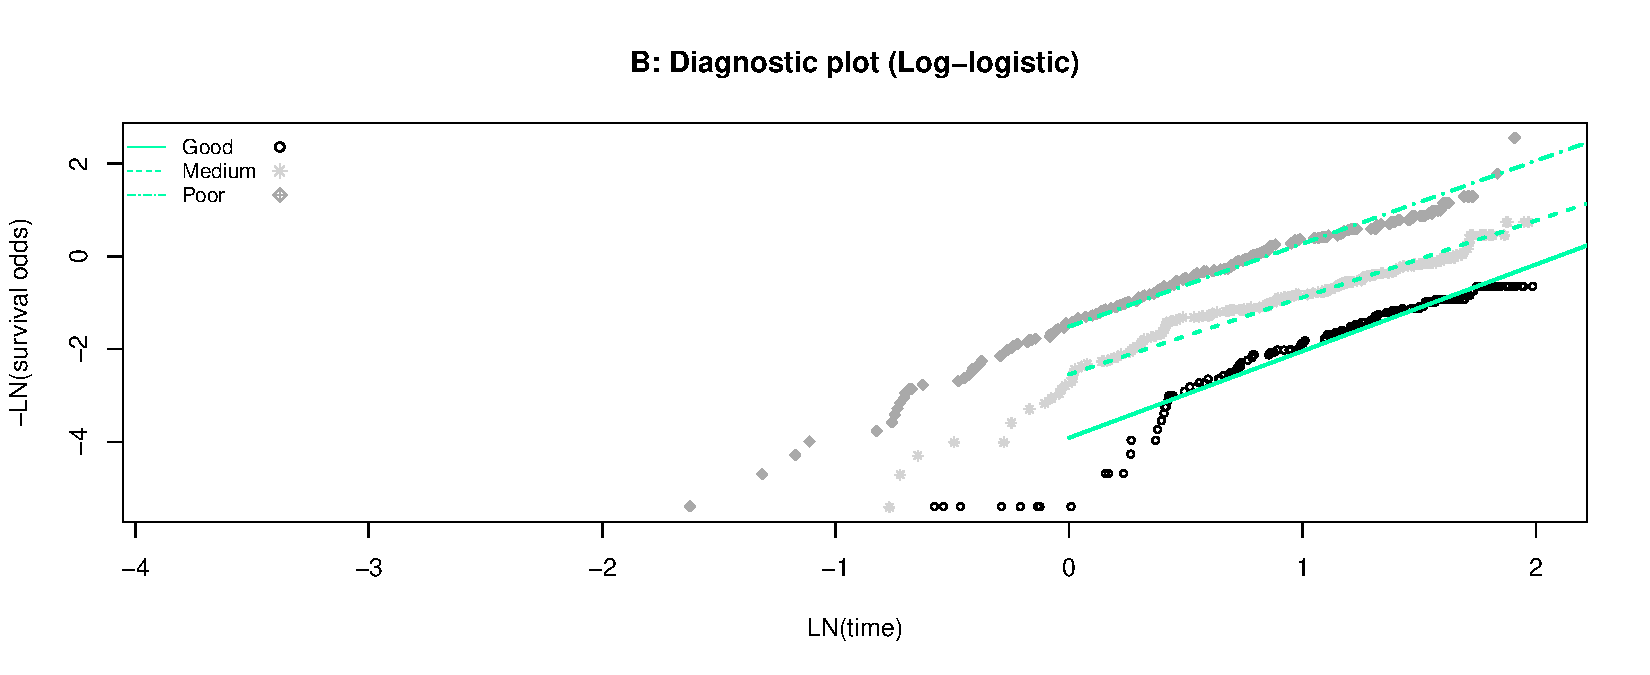
\includegraphics[height=0.25\textheight]{C:/Users/g10028783/Downloads/R talks/PERSUADE//tests/testthat/grid_test/check_20_output/Images/Figure_param_models-14} \end{flushleft}

\begin{flushleft}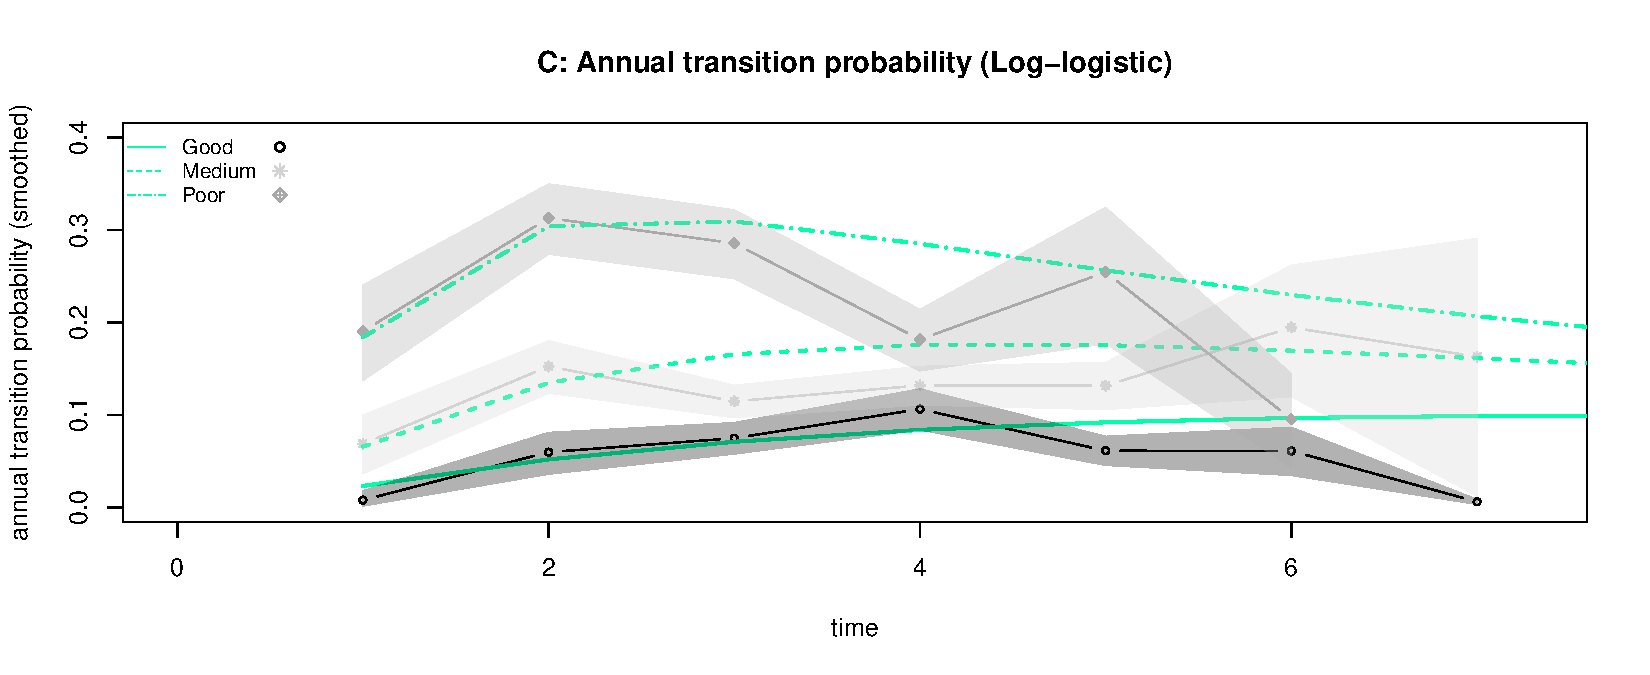
\includegraphics[height=0.25\textheight]{C:/Users/g10028783/Downloads/R talks/PERSUADE//tests/testthat/grid_test/check_20_output/Images/Figure_param_models-15} \end{flushleft}

\clearpage

\subsubsection{Gamma}\label{gamma}

\begin{flushleft}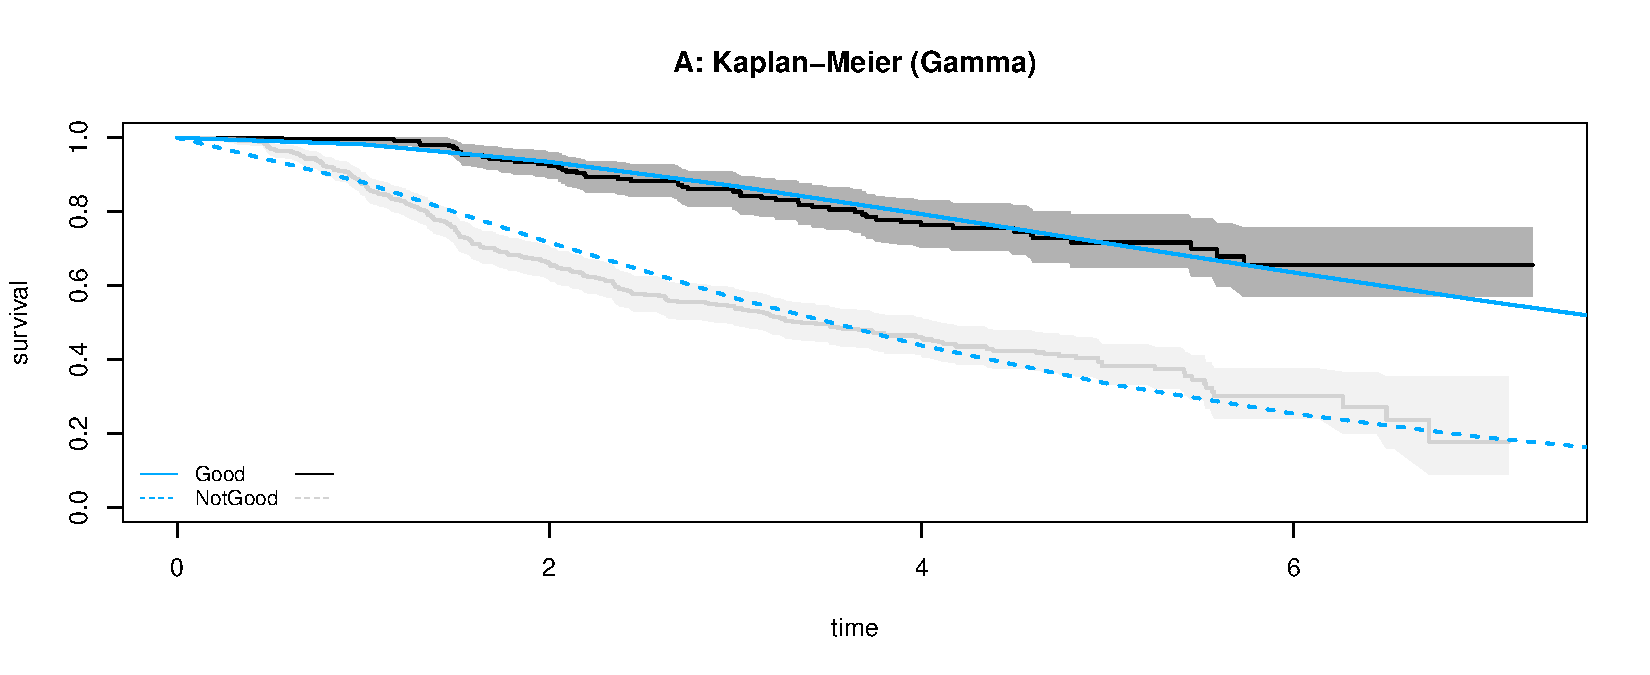
\includegraphics[height=0.25\textheight]{C:/Users/g10028783/Downloads/R talks/PERSUADE//tests/testthat/grid_test/check_20_output/Images/Figure_param_models-16} \end{flushleft}

\begin{flushleft}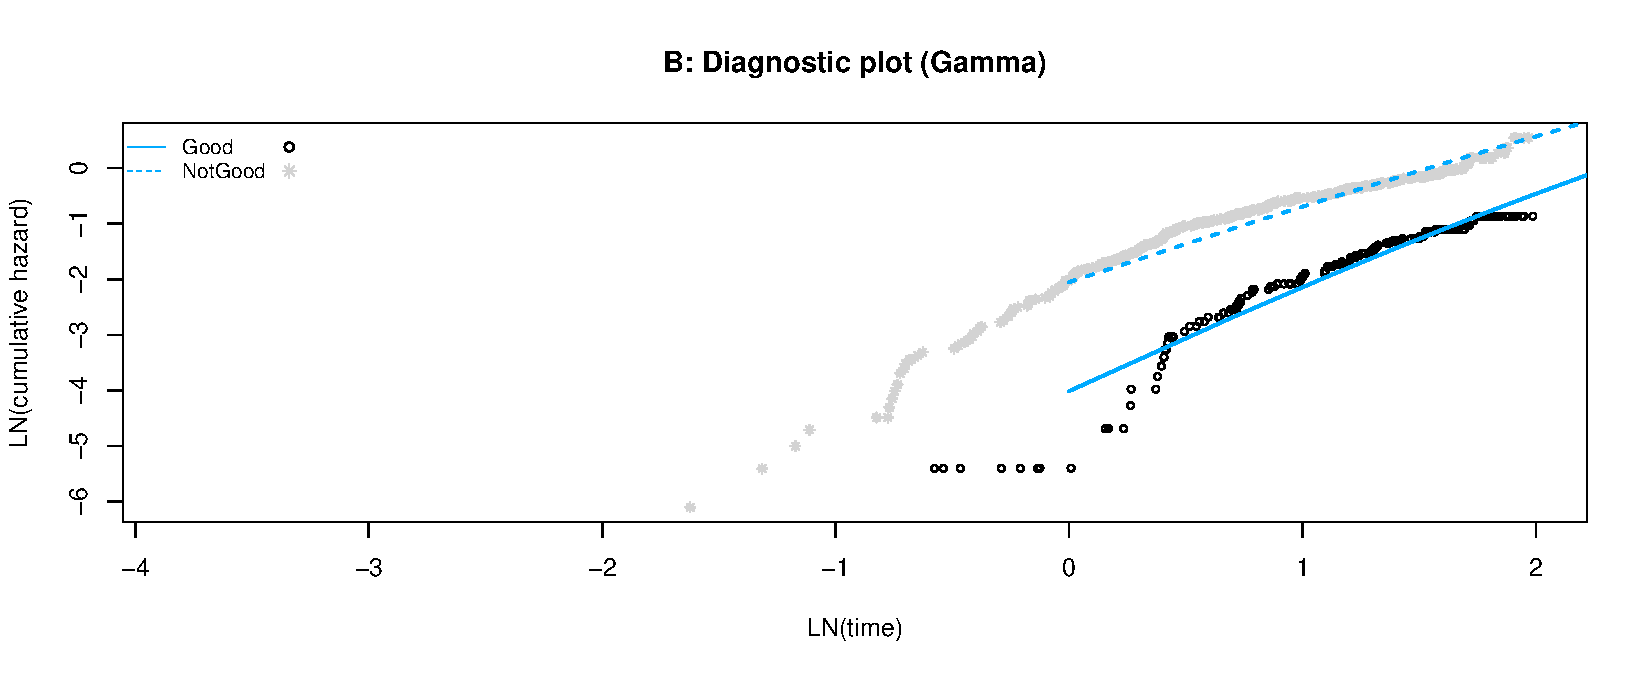
\includegraphics[height=0.25\textheight]{C:/Users/g10028783/Downloads/R talks/PERSUADE//tests/testthat/grid_test/check_20_output/Images/Figure_param_models-17} \end{flushleft}

\begin{flushleft}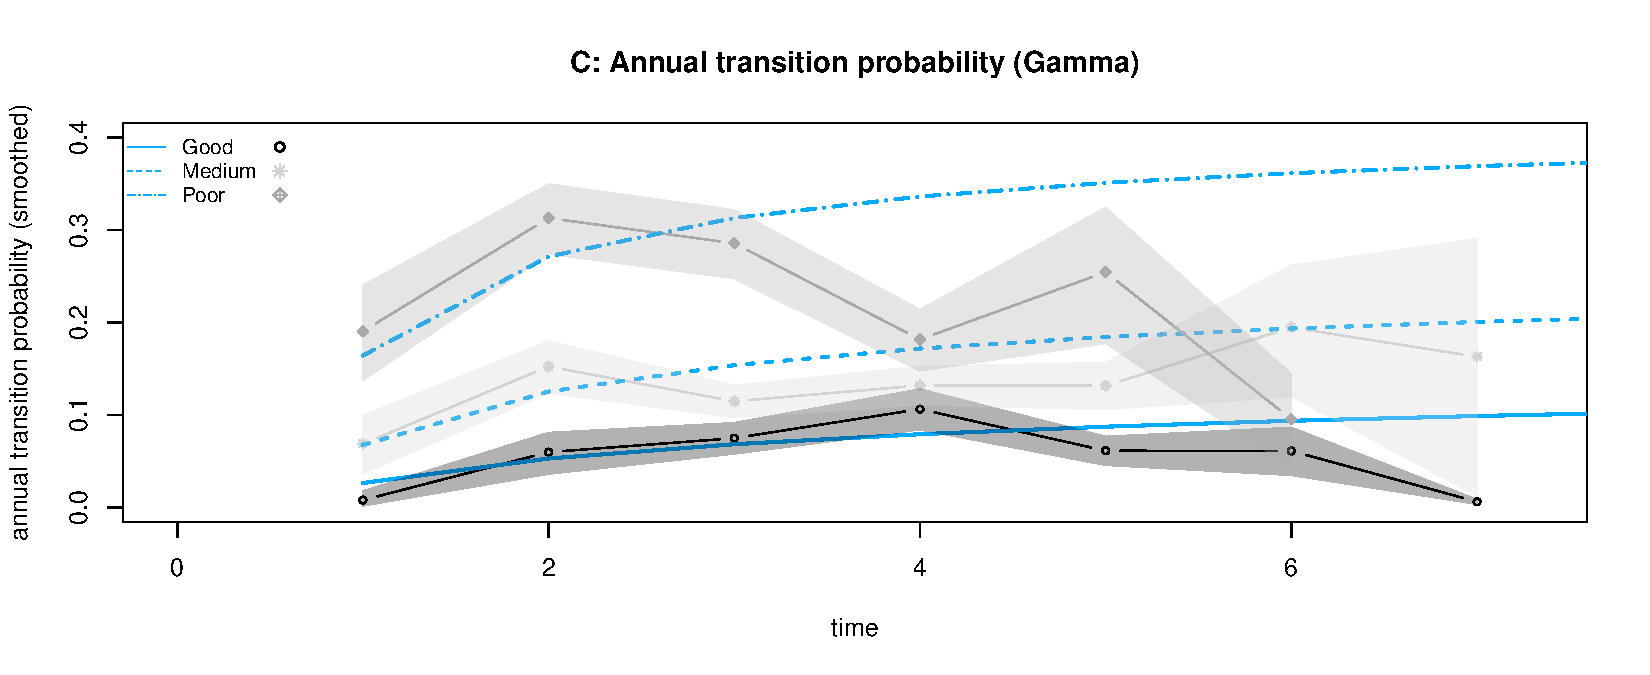
\includegraphics[height=0.25\textheight]{C:/Users/g10028783/Downloads/R talks/PERSUADE//tests/testthat/grid_test/check_20_output/Images/Figure_param_models-18} \end{flushleft}

\clearpage

\subsubsection{Generalised Gamma}\label{generalised-gamma}

\begin{flushleft}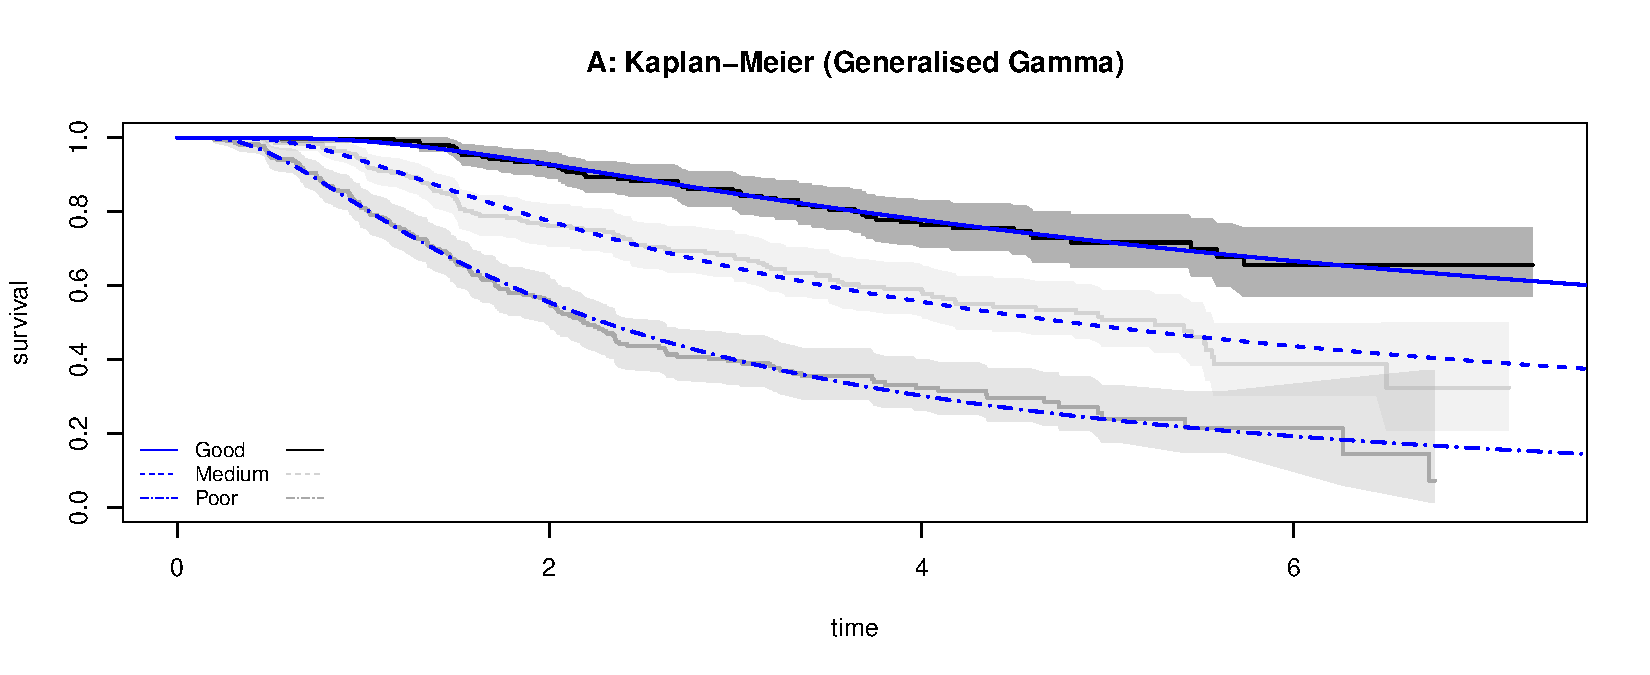
\includegraphics[height=0.25\textheight]{C:/Users/g10028783/Downloads/R talks/PERSUADE//tests/testthat/grid_test/check_20_output/Images/Figure_param_models-19} \end{flushleft}

\begin{flushleft}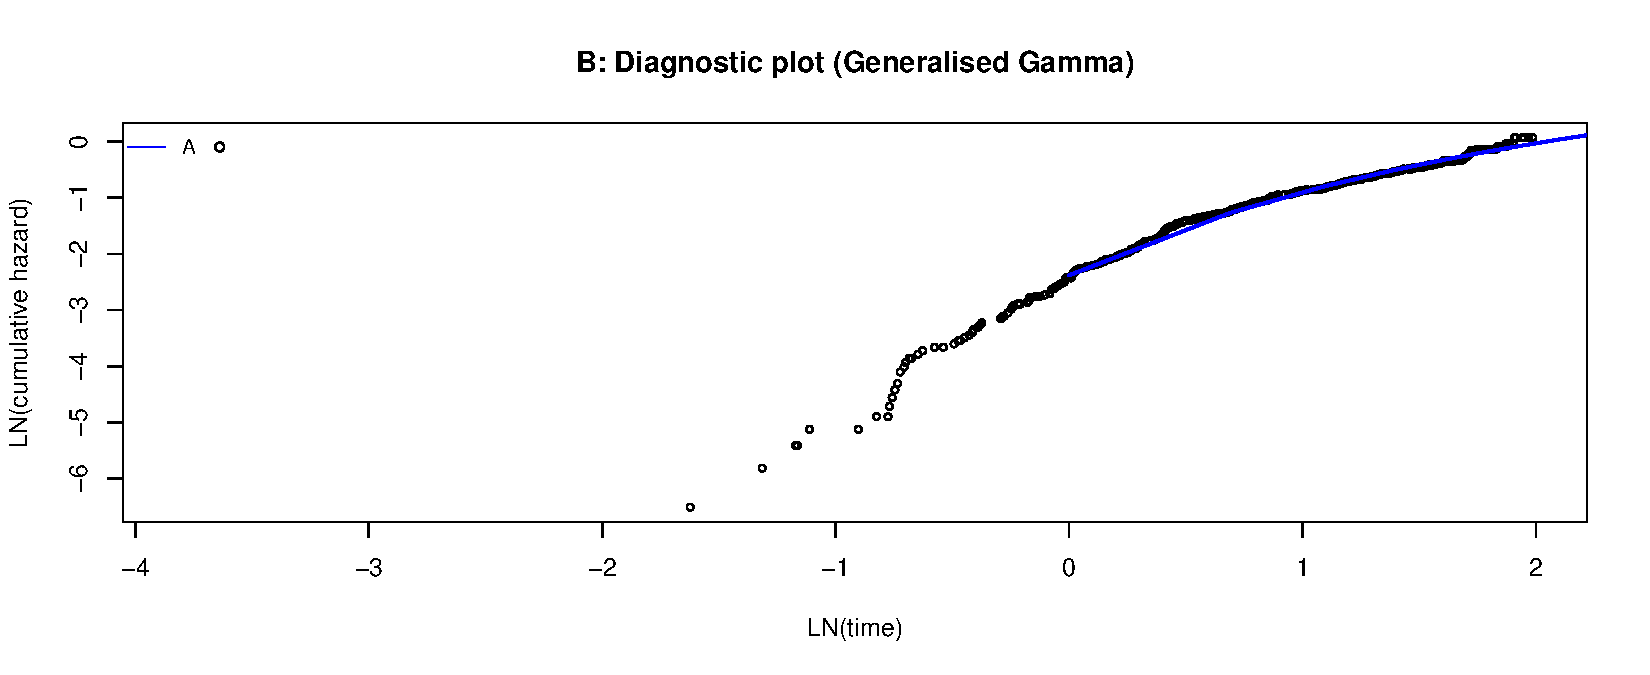
\includegraphics[height=0.25\textheight]{C:/Users/g10028783/Downloads/R talks/PERSUADE//tests/testthat/grid_test/check_20_output/Images/Figure_param_models-20} \end{flushleft}

\begin{flushleft}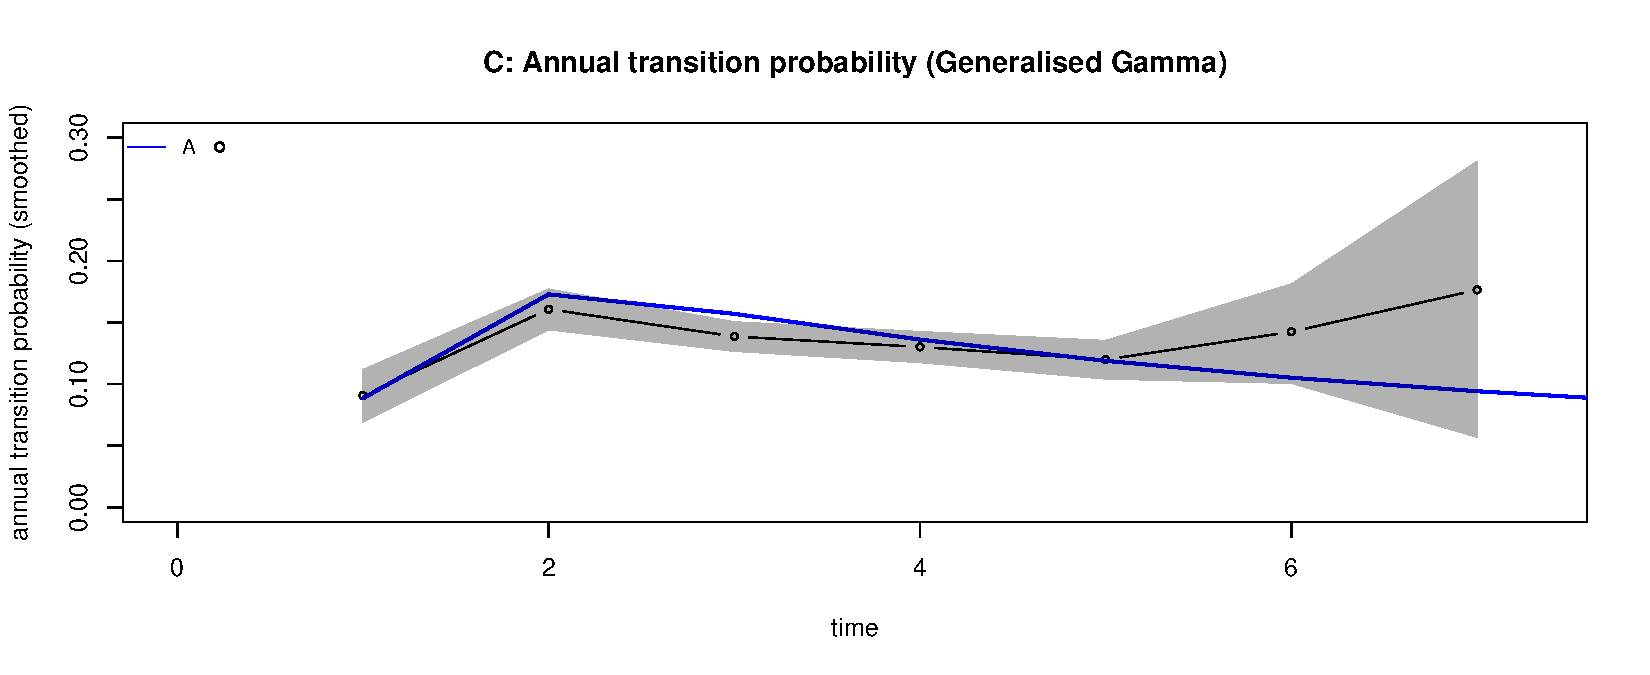
\includegraphics[height=0.25\textheight]{C:/Users/g10028783/Downloads/R talks/PERSUADE//tests/testthat/grid_test/check_20_output/Images/Figure_param_models-21} \end{flushleft}

\clearpage

\subsection{4.2 Parametric natural cubic spline
models}\label{parametric-natural-cubic-spline-models}

If standard parametric models do not provide a satisfactory fit to the
data (based on the visual assessments and goodness-of-fit statistics
presented in the previous section or extrapolations presented in the
next section), spline-based models may provide a more flexible
alternative. An explanation of these natural cubic spline models,
henceforth referred to as spline-based models, is provided in
\href{https://doi.org/10.1002/sim.1203}{Royston and Parmar (2002)}.

\textbf{Model complexity and parsimony}\\
Following the principle of \emph{Occam's Razor} and the recommendations
in
\href{https://www.sheffield.ac.uk/media/34188/download?attachment}{NICE
TSD 21}, the preferred approach is to select the simplest model (e.g., a
standard parametric model) that provides an adequate fit to the data and
clinically plausible extrapolations. However, when simpler models do not
provide a satisfactory fit, particularly in terms of long-term
extrapolations and consistency with external evidence, more flexible
models, such as spline-based models, can be considered.

\textbf{Relationship to standard parametric models}\\
Spline-based models extend standard parametric survival models by
allowing the hazard, odds, or normal scale to vary flexibly over time:

\begin{itemize}
\tightlist
\item
  \textbf{Hazard scale} spline models extend the Weibull distribution.\\
\item
  \textbf{Odds scale} spline models extend the log-logistic
  distribution.\\
\item
  \textbf{Normal scale} spline models extend the log-normal
  distribution.
\end{itemize}

\textbf{Model assessment and rules of thumb}\\
The same goodness-of-fit statistics (AIC and BIC) used in Section 4.1
are presented here, and the same \emph{rules of thumb} apply:

\begin{itemize}
\tightlist
\item
  \textbf{Burnham \& Anderson (1998)}: Models within 4 AIC points of the
  lowest AIC are considered to have substantial support from the data
  \href{https://doi.org/10.1007/978-1-4757-2917-7}{Burnham and Anderson,
  1998}.\\
\item
  \textbf{Raftery (1995)}: Models within 2 BIC points of the lowest BIC
  are considered among the best-fitting models
  \href{https://doi.org/10.2307/271063}{Raftery et al., 1995}.
\end{itemize}

\textbf{Plots}\\
As in Section 4.1, the following pages display three plots for each
fitted spline-based survival model:

\begin{itemize}
\tightlist
\item
  \textbf{Figure A}: Kaplan--Meier curves (black and grey) versus the
  fitted spline model (colour).\\
\item
  \textbf{Figure B}: Model-specific diagnostic plots (see
  \href{https://doi.org/10.1007/s40273-013-0064-3}{Ishak et al.,
  2013}).\\
\item
  \textbf{Figure C}: Smoothed hazard rates from empirical data (black
  and grey) versus model-based estimates (colour).
\end{itemize}

\textbf{CAUTION}:\\
These statistics and plots apply only to the \emph{observed} data period
and do not directly inform the appropriateness of extrapolations beyond
this period.\\
Additionally, the tail of the observed data may be affected by a low
number of events, which should be considered when interpreting model
performance.

\clearpage

\clearpage

\subsection{4.3 Parametric (non-)mixture cure
models}\label{parametric-non-mixture-cure-models}

In some disease areas, a proportion of patients may be considered
``cured,'' meaning they have the same mortality risk as the general
population (or a background hazard). Cure models explicitly allow for
this possibility and estimate both the cure fraction and the survival of
the uncured fraction.

\begin{itemize}
\tightlist
\item
  \emph{Mixture cure models}: Assume the population is composed of a
  cured fraction and an uncured fraction, each with its own survival
  curve. The overall survival curve is a weighted mixture of the two.
  This means the survival curve approaches a horizontal asymptote at the
  estimated cure fraction.\\
\item
  \emph{Non-mixture cure models}: Directly model the hazard function so
  that it approaches zero over time for the cured fraction, without
  explicitly separating the two subpopulations in the survival function.
\end{itemize}

Both approaches can be fitted using standard parametric distributions
(i.e., Weibull, log-normal or log-logistic).

The \emph{link function} relates the linear predictor to the estimated
cure fraction.\\
The most commonly used link function is the \emph{logistic}, but others
are available:

\begin{itemize}
\tightlist
\item
  \texttt{"logistic"}: Ensures the cure fraction is between 0 and 1 via
  the logistic transformation.\\
\item
  \texttt{"loglog"}: Uses the complementary log--log link, which can be
  more appropriate if cure proportions are very close to 0 or 1.\\
\item
  \texttt{"identity"}: Fits the cure fraction directly on the
  probability scale (must remain in {[}0,1{]}).\\
\item
  \texttt{"probit"}: Uses the cumulative normal distribution as the
  link.
\end{itemize}

\textbf{Model complexity and parsimony}\\
Following \emph{Occam's Razor} and
\href{https://www.sheffield.ac.uk/media/34188/download?attachment}{NICE
TSD 21}, standard parametric models should be preferred when they
provide an adequate and clinically plausible fit. Cure models should be
considered only when there is strong clinical or empirical evidence
supporting the presence of a long-term cured fraction.

\textbf{Model assessment and rules of thumb}\\
The same goodness-of-fit statistics (AIC and BIC) used in Section 4.1
are presented here, and the same \emph{rules of thumb} apply:

\begin{itemize}
\tightlist
\item
  \textbf{Burnham \& Anderson (1998)}: Models within 4 AIC points of the
  lowest AIC are considered to have substantial support from the data
  \href{https://doi.org/10.1007/978-1-4757-2917-7}{Burnham and Anderson,
  1998}.\\
\item
  \textbf{Raftery (1995)}: Models within 2 BIC points of the lowest BIC
  are considered among the best-fitting models
  \href{https://doi.org/10.2307/271063}{Raftery et al., 1995}.
\end{itemize}

\textbf{Plots}\\
As in Section 4.1, the following pages display three plots for each
fitted spline-based survival model:

\begin{itemize}
\tightlist
\item
  \textbf{Figure A}: Kaplan--Meier curves (black and grey) versus the
  fitted spline model (colour).\\
\item
  \textbf{Figure B}: Model-specific diagnostic plots (see
  \href{https://doi.org/10.1007/s40273-013-0064-3}{Ishak et al.,
  2013}).\\
\item
  \textbf{Figure C}: Smoothed hazard rates from empirical data (black
  and grey) versus model-based estimates (colour).
\end{itemize}

\textbf{CAUTION}:\\
These statistics and plots apply only to the \emph{observed} data period
and do not directly inform the appropriateness of extrapolations beyond
this period.\\
Additionally, the tail of the observed data may be affected by a low
number of events, which should be considered when interpreting model
performance.

\clearpage

\begin{table}[H]
\centering
\caption{\label{tab:Table_4}Goodness of fit statistics (including standard parametric and cure models)}
\centering
\resizebox{\ifdim\width>\linewidth\linewidth\else\width\fi}{!}{
\begin{tabular}[t]{lr}
\toprule
Model & AIC\\
\midrule
\cellcolor{gray!10}{Generalised Gamma} & \cellcolor{gray!10}{1619}\\
Non-mixture cure Log-normal & 1626\\
\cellcolor{gray!10}{Mixture cure Log-normal} & \cellcolor{gray!10}{1626}\\
Log-normal & 1627\\
\cellcolor{gray!10}{Mixture cure Log-logistic} & \cellcolor{gray!10}{1637}\\
Non-mixture cure Log-logistic & 1638\\
\cellcolor{gray!10}{Log-logistic} & \cellcolor{gray!10}{1646}\\
Non-mixture cure Weibull & 1648\\
\cellcolor{gray!10}{Mixture cure Weibull} & \cellcolor{gray!10}{1655}\\
Gamma & 1660\\
\cellcolor{gray!10}{Weibull} & \cellcolor{gray!10}{1671}\\
Gompertz & 1694\\
\cellcolor{gray!10}{Exponential} & \cellcolor{gray!10}{1698}\\
\bottomrule
\end{tabular}}
\end{table}

\begin{table}[H]
\centering
\caption{\label{tab:Table_5}Cure proportions per group (lower and upper 95CI)}
\centering
\resizebox{\ifdim\width>\linewidth\linewidth\else\width\fi}{!}{
\begin{tabular}[t]{ll}
\toprule
Model & CureFraction\\
\midrule
\cellcolor{gray!10}{Mixture cure Weibull} & \cellcolor{gray!10}{65\% (75\%–53\%), 27\% (36\%–18\%)}\\
Non-mixture cure Weibull & 65\% (75\%–53\%), 26\% (35\%–17\%)\\
\cellcolor{gray!10}{Mixture cure Log-normal} & \cellcolor{gray!10}{57\% (76\%–33\%), 18\% (33\%–7\%)}\\
Non-mixture cure Log-normal & 56\% (76\%–30\%), 17\% (31\%–7\%)\\
\cellcolor{gray!10}{Mixture cure Log-logistic} & \cellcolor{gray!10}{60\% (74\%–43\%), 22\% (33\%–12\%)}\\
Non-mixture cure Log-logistic & 60\% (74\%–44\%), 23\% (33\%–14\%)\\
\bottomrule
\end{tabular}}
\end{table}

\clearpage

\clearpage

\subsubsection{Mixture cure Weibull}\label{mixture-cure-weibull}

\begin{flushleft}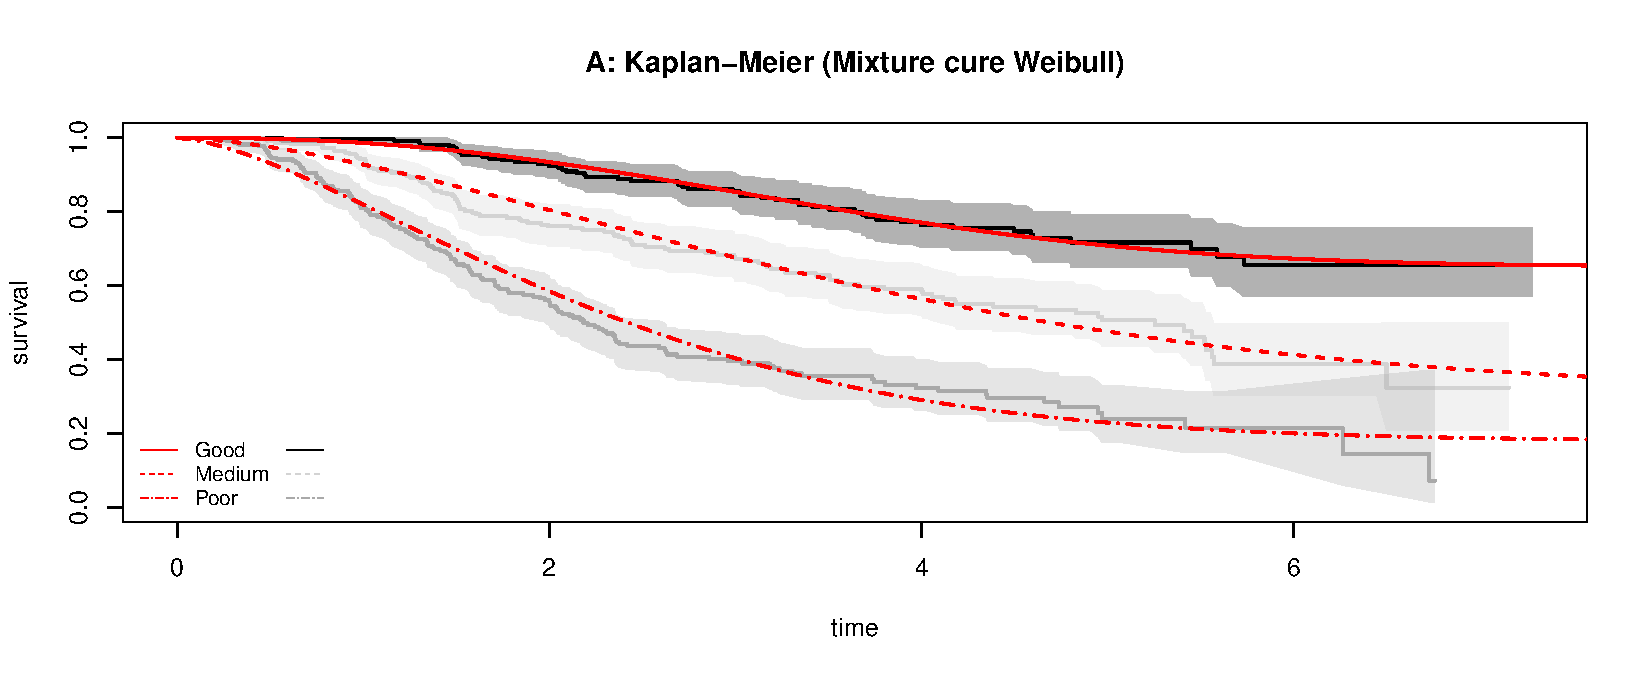
\includegraphics[height=0.25\textheight]{C:/Users/g10028783/Downloads/R talks/PERSUADE//tests/testthat/grid_test/check_20_output/Images/Figure_cure_models-1} \end{flushleft}

\begin{flushleft}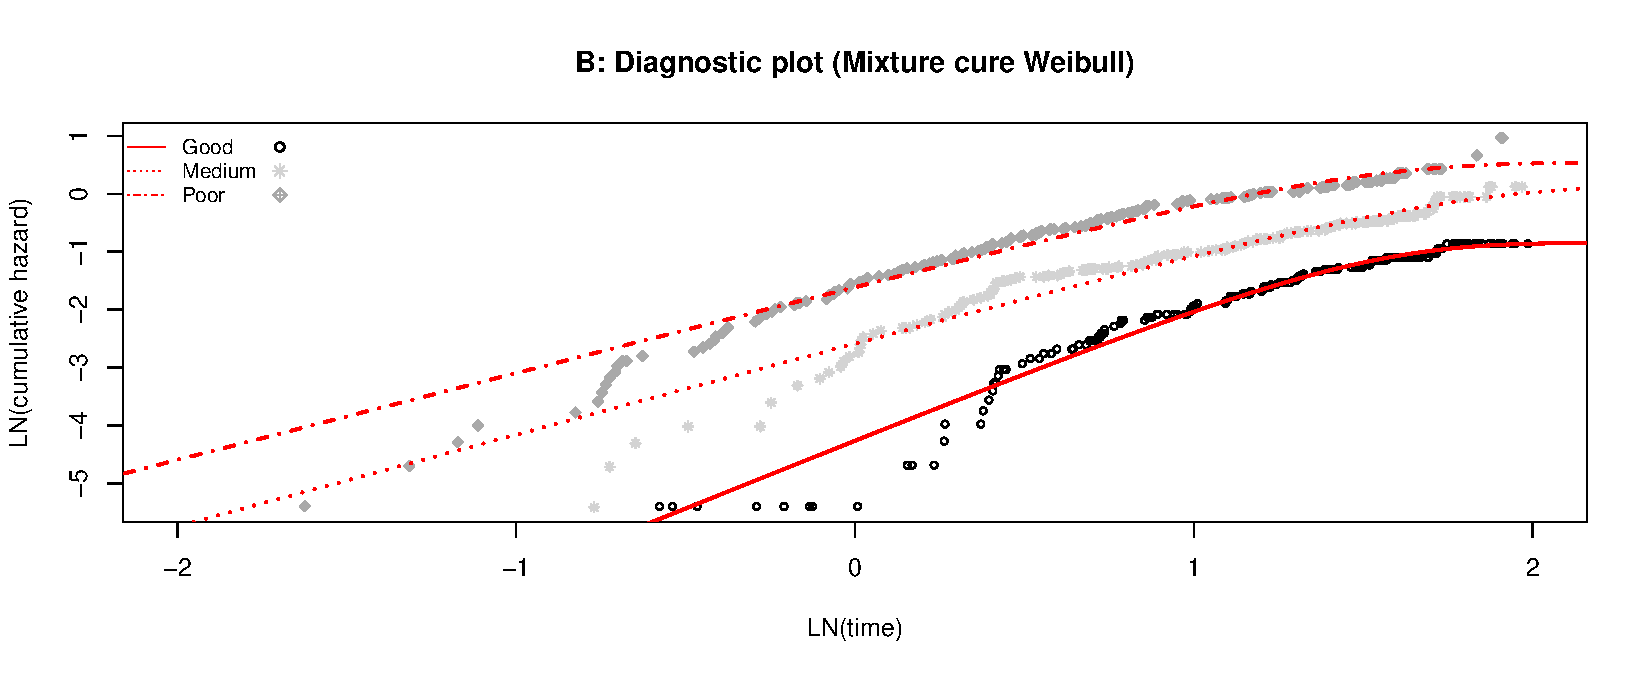
\includegraphics[height=0.25\textheight]{C:/Users/g10028783/Downloads/R talks/PERSUADE//tests/testthat/grid_test/check_20_output/Images/Figure_cure_models-2} \end{flushleft}

\begin{flushleft}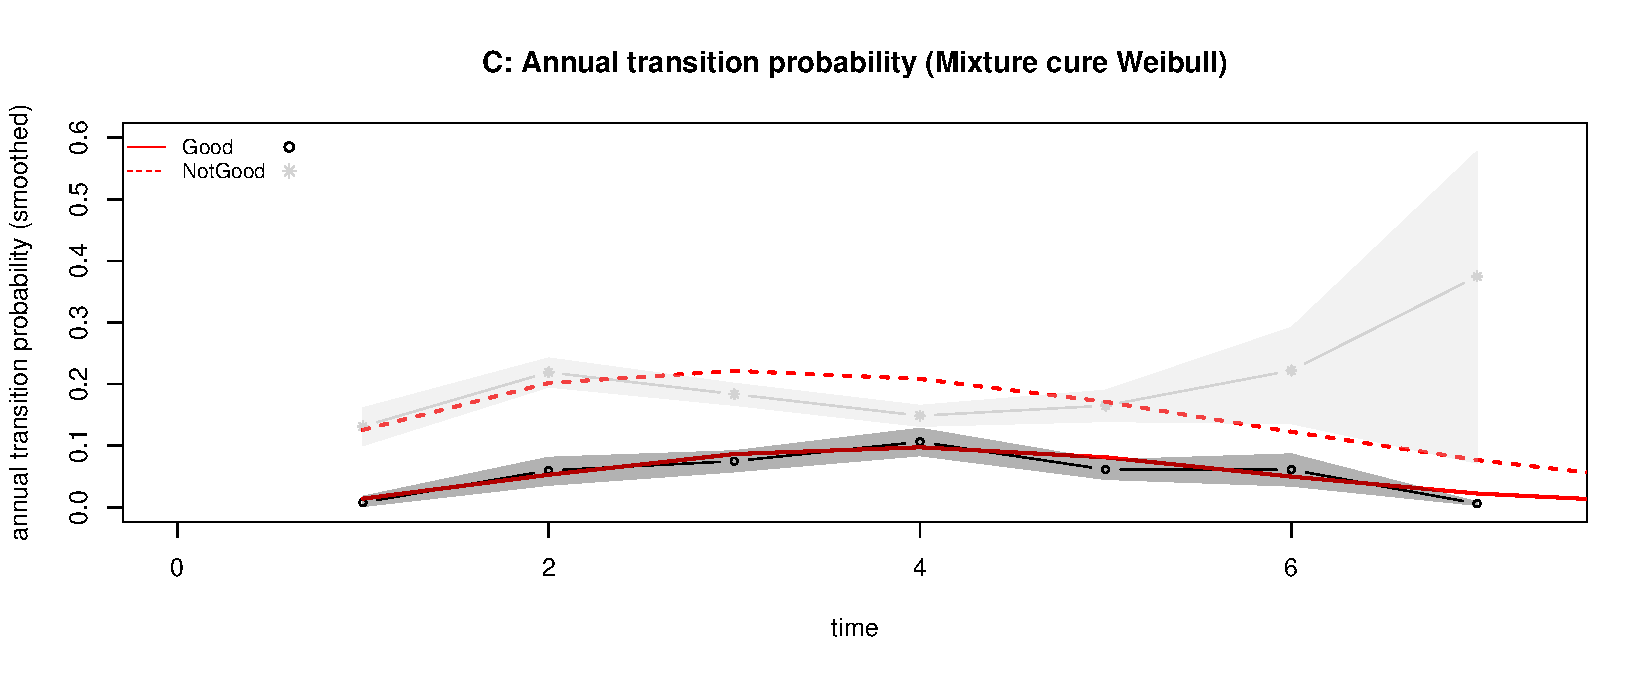
\includegraphics[height=0.25\textheight]{C:/Users/g10028783/Downloads/R talks/PERSUADE//tests/testthat/grid_test/check_20_output/Images/Figure_cure_models-3} \end{flushleft}

\clearpage

\subsubsection{Non-mixture cure Weibull}\label{non-mixture-cure-weibull}

\begin{flushleft}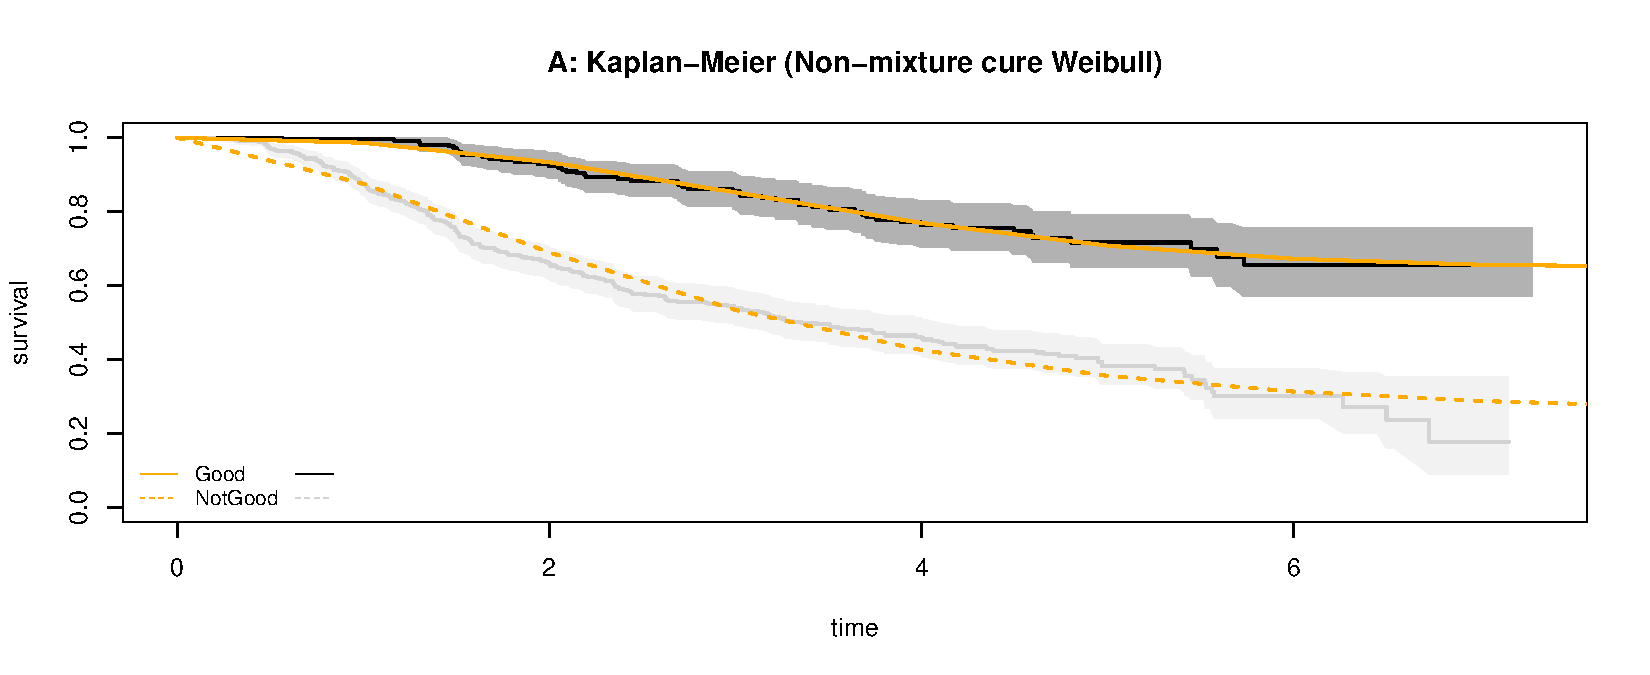
\includegraphics[height=0.25\textheight]{C:/Users/g10028783/Downloads/R talks/PERSUADE//tests/testthat/grid_test/check_20_output/Images/Figure_cure_models-4} \end{flushleft}

\begin{flushleft}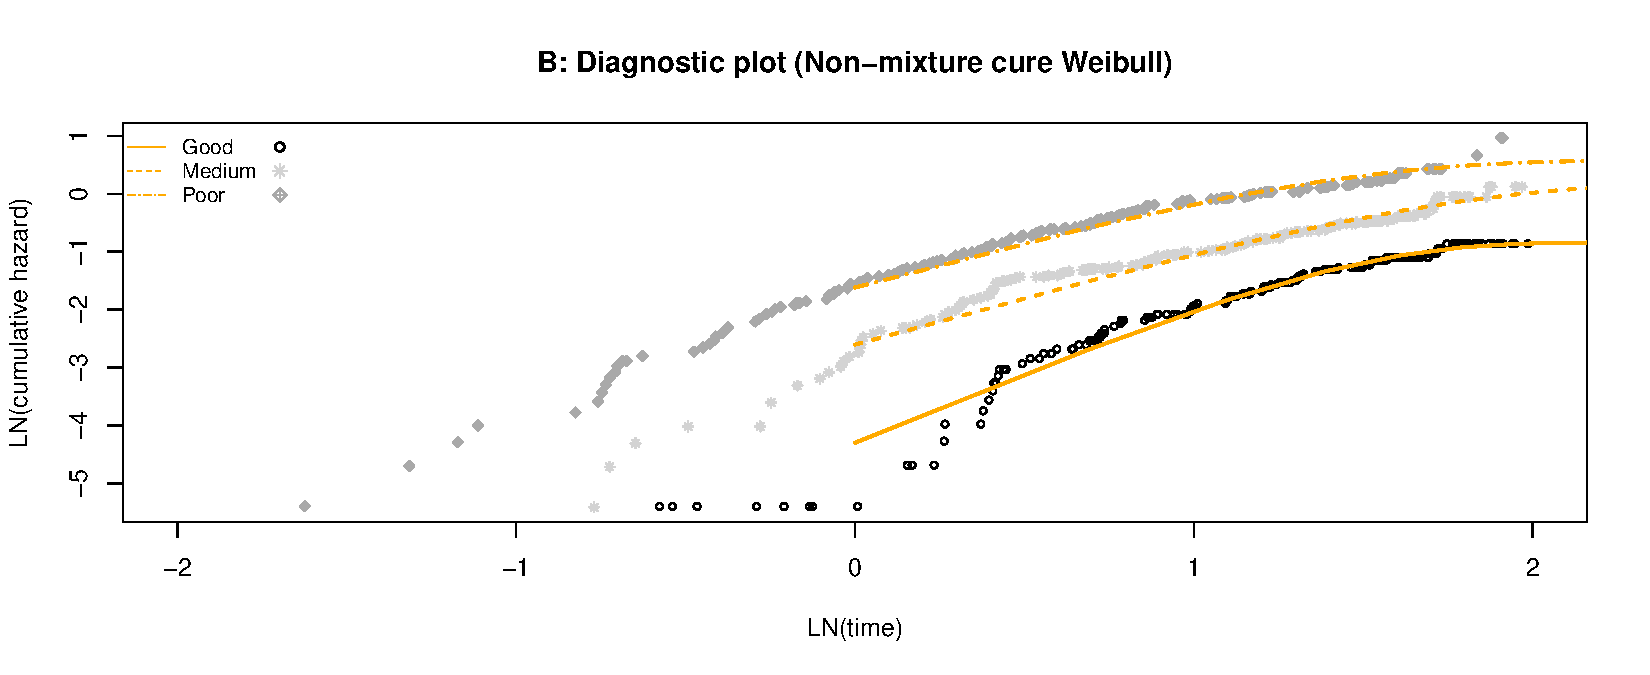
\includegraphics[height=0.25\textheight]{C:/Users/g10028783/Downloads/R talks/PERSUADE//tests/testthat/grid_test/check_20_output/Images/Figure_cure_models-5} \end{flushleft}

\begin{flushleft}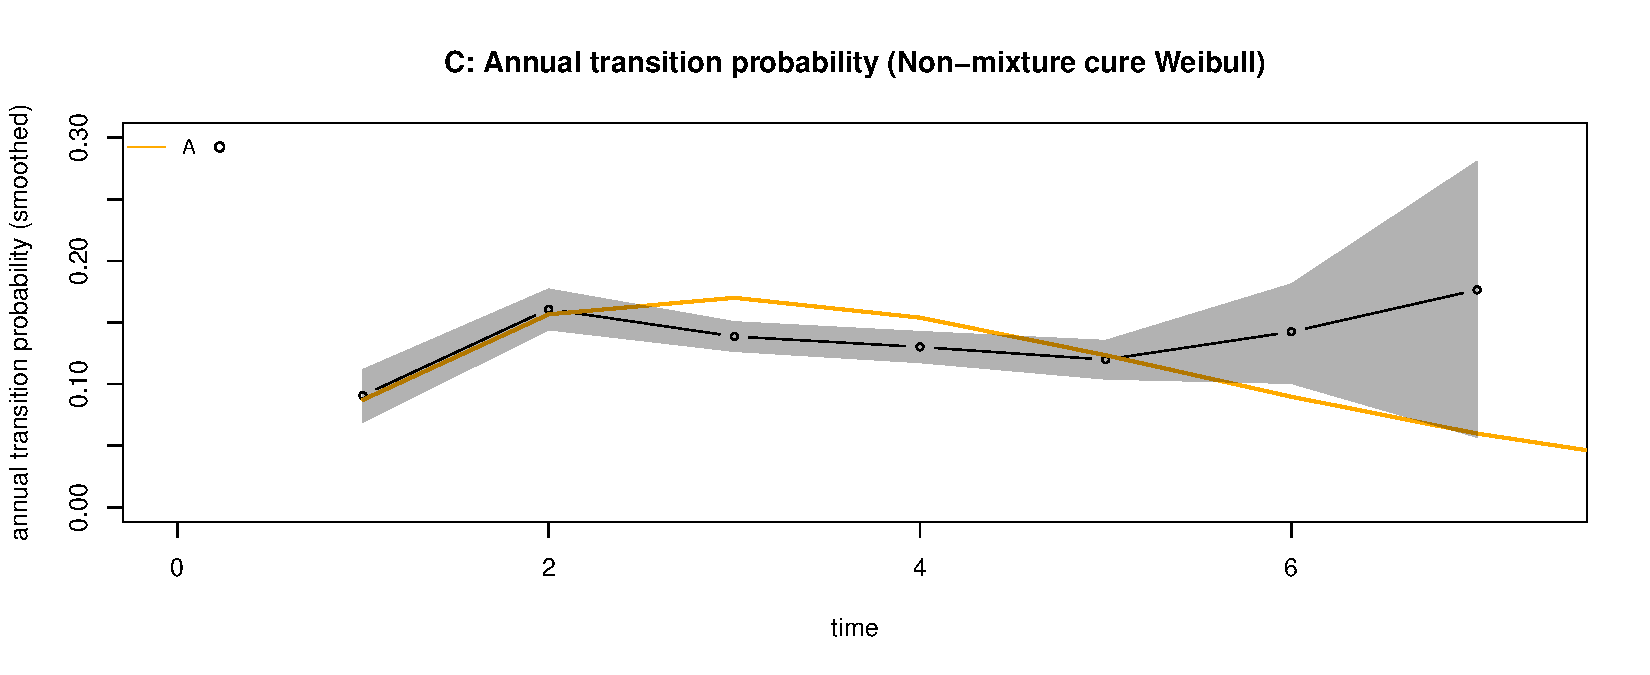
\includegraphics[height=0.25\textheight]{C:/Users/g10028783/Downloads/R talks/PERSUADE//tests/testthat/grid_test/check_20_output/Images/Figure_cure_models-6} \end{flushleft}

\clearpage

\subsubsection{Mixture cure Log-normal}\label{mixture-cure-log-normal}

\begin{flushleft}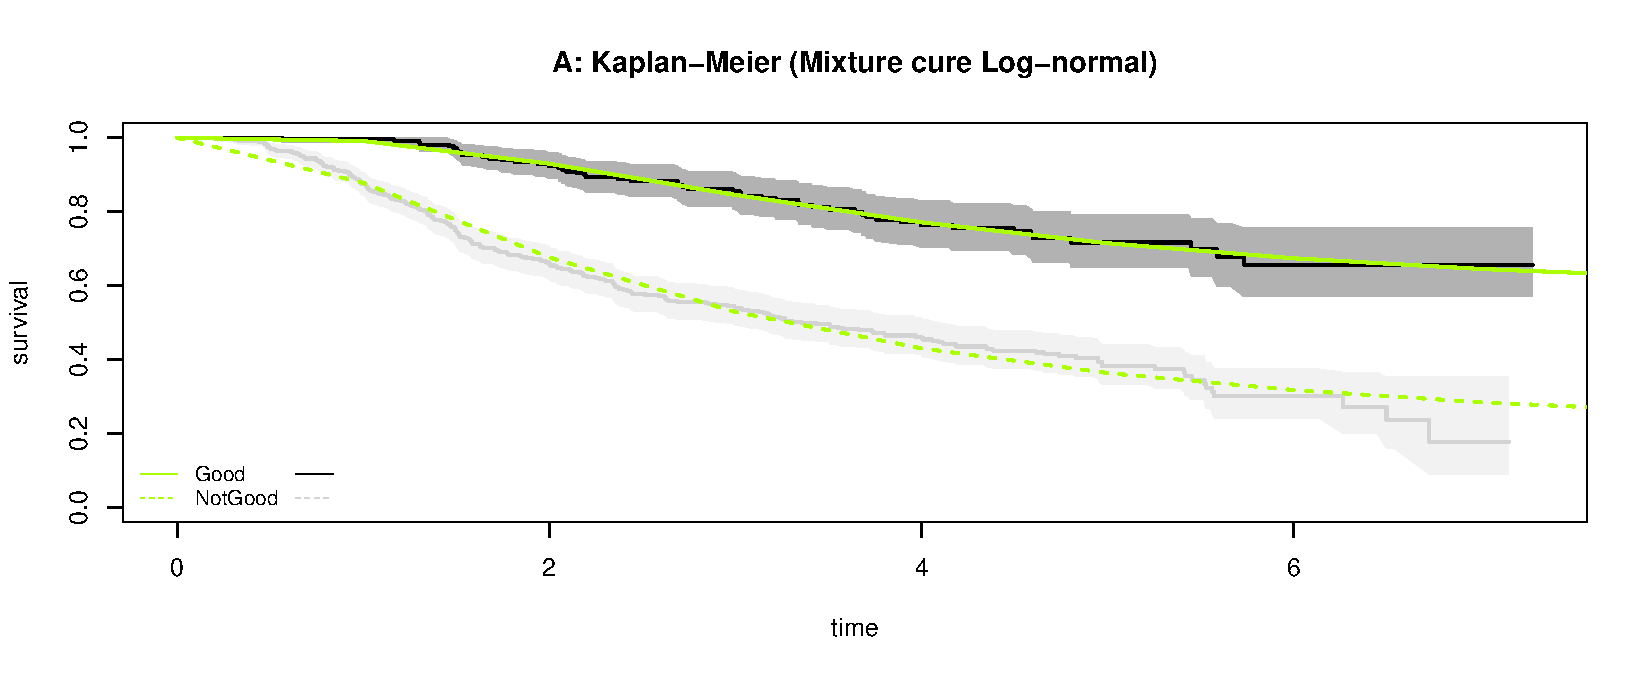
\includegraphics[height=0.25\textheight]{C:/Users/g10028783/Downloads/R talks/PERSUADE//tests/testthat/grid_test/check_20_output/Images/Figure_cure_models-7} \end{flushleft}

\begin{flushleft}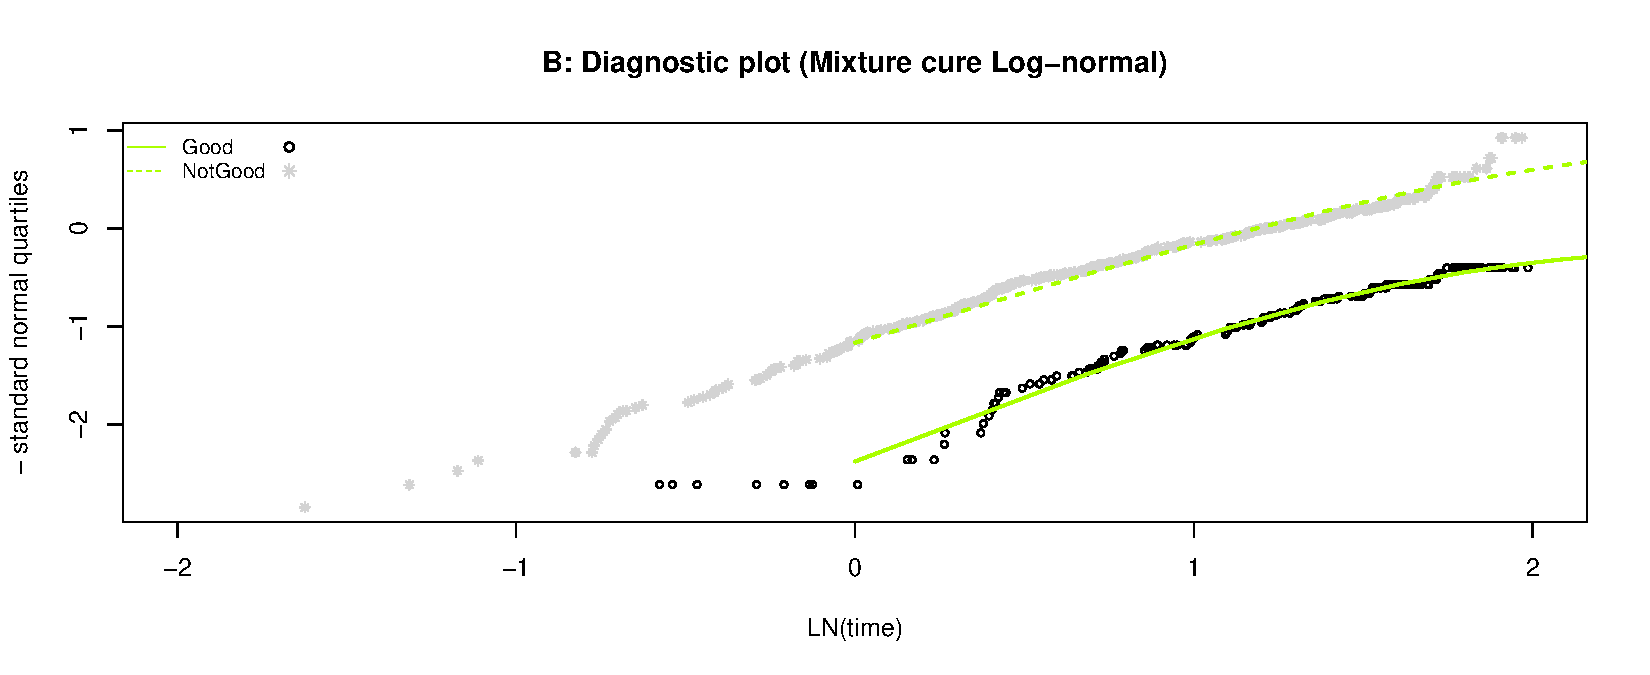
\includegraphics[height=0.25\textheight]{C:/Users/g10028783/Downloads/R talks/PERSUADE//tests/testthat/grid_test/check_20_output/Images/Figure_cure_models-8} \end{flushleft}

\begin{flushleft}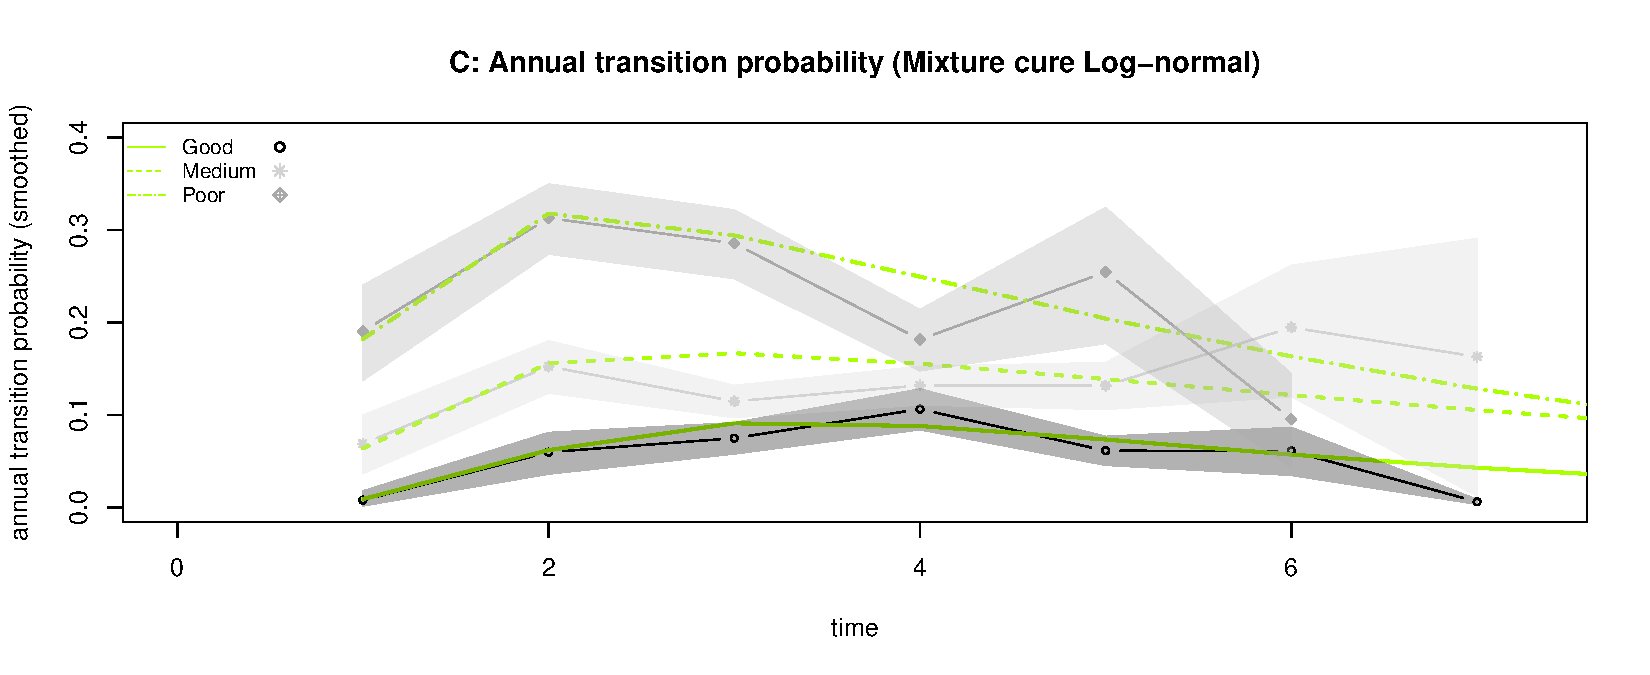
\includegraphics[height=0.25\textheight]{C:/Users/g10028783/Downloads/R talks/PERSUADE//tests/testthat/grid_test/check_20_output/Images/Figure_cure_models-9} \end{flushleft}

\clearpage

\subsubsection{Non-mixture cure
Log-normal}\label{non-mixture-cure-log-normal}

\begin{flushleft}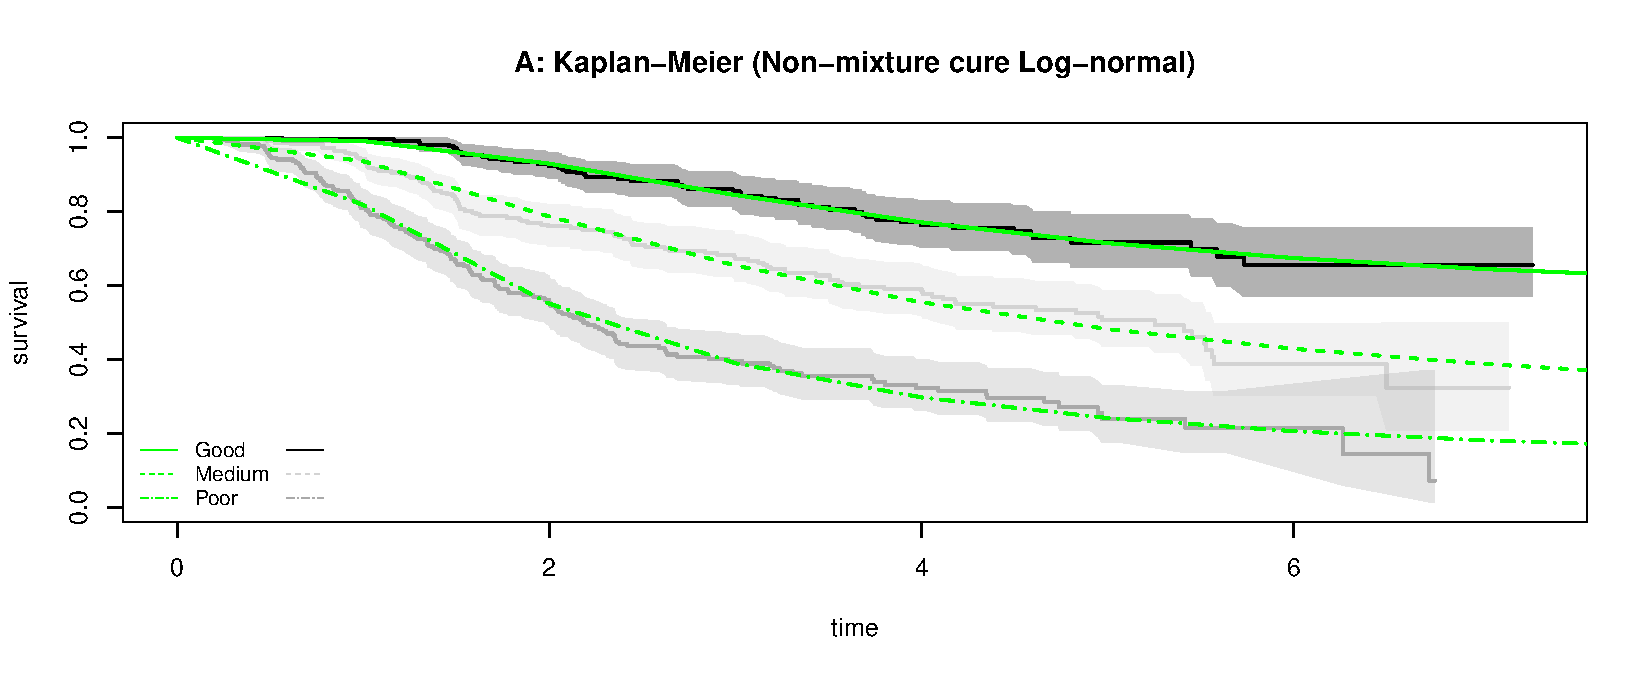
\includegraphics[height=0.25\textheight]{C:/Users/g10028783/Downloads/R talks/PERSUADE//tests/testthat/grid_test/check_20_output/Images/Figure_cure_models-10} \end{flushleft}

\begin{flushleft}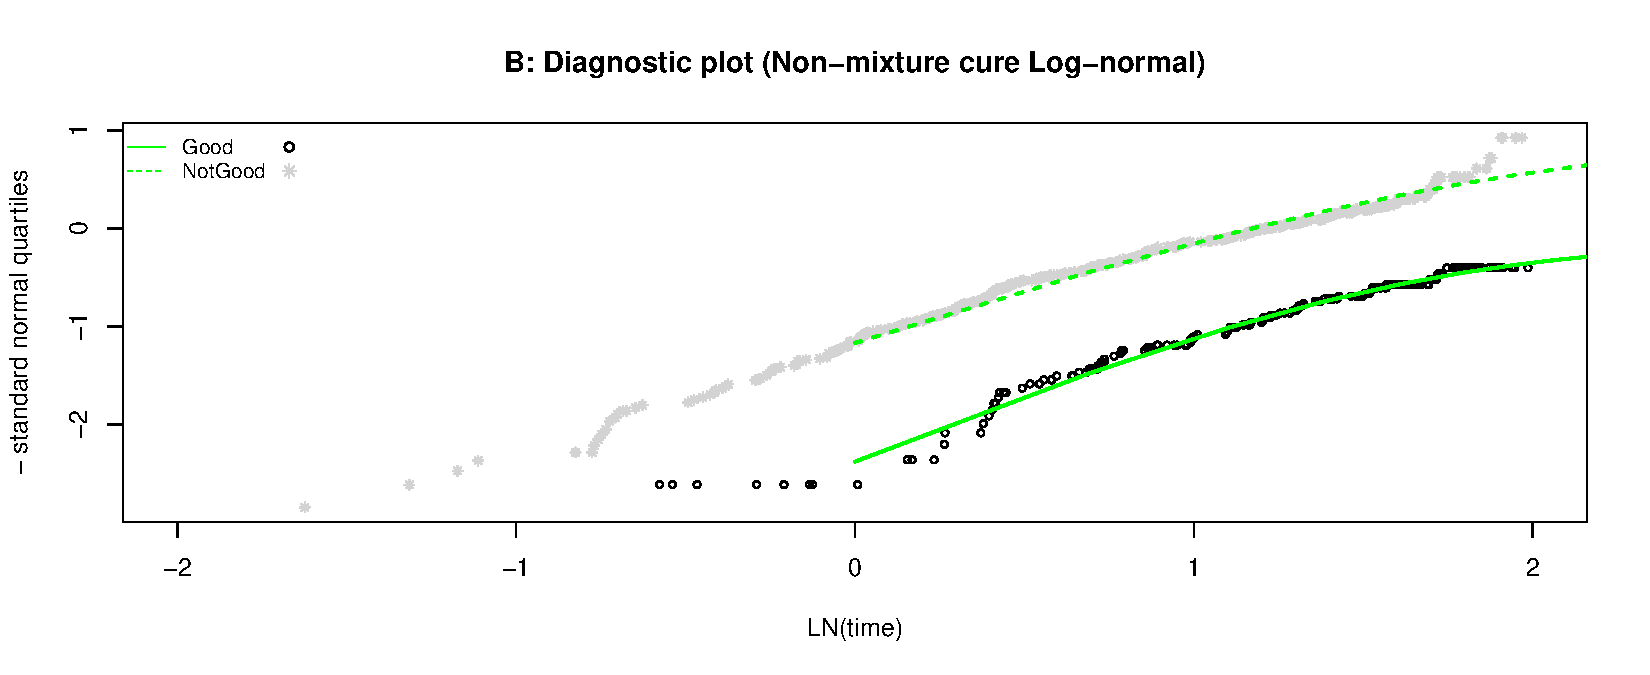
\includegraphics[height=0.25\textheight]{C:/Users/g10028783/Downloads/R talks/PERSUADE//tests/testthat/grid_test/check_20_output/Images/Figure_cure_models-11} \end{flushleft}

\begin{flushleft}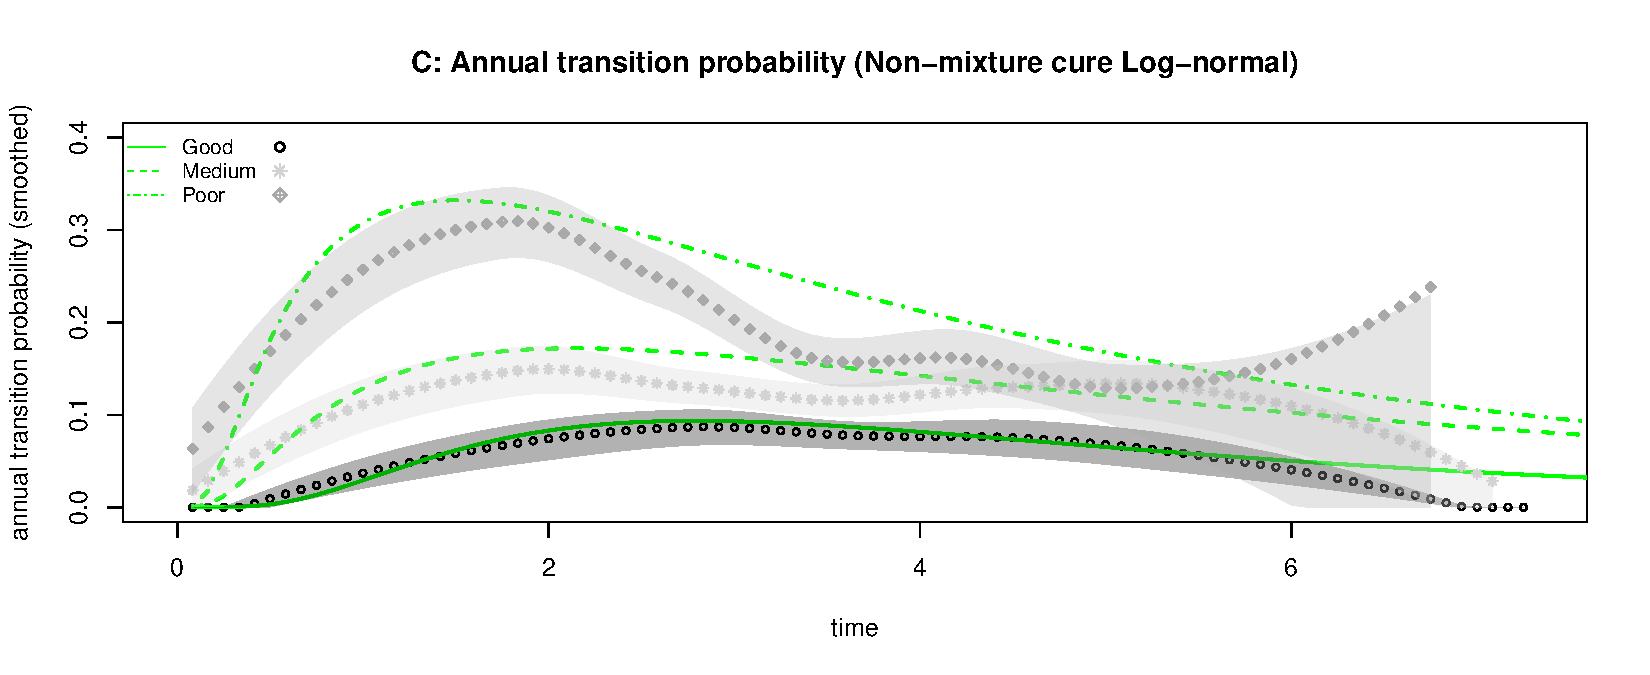
\includegraphics[height=0.25\textheight]{C:/Users/g10028783/Downloads/R talks/PERSUADE//tests/testthat/grid_test/check_20_output/Images/Figure_cure_models-12} \end{flushleft}

\clearpage

\subsubsection{Mixture cure
Log-logistic}\label{mixture-cure-log-logistic}

\begin{flushleft}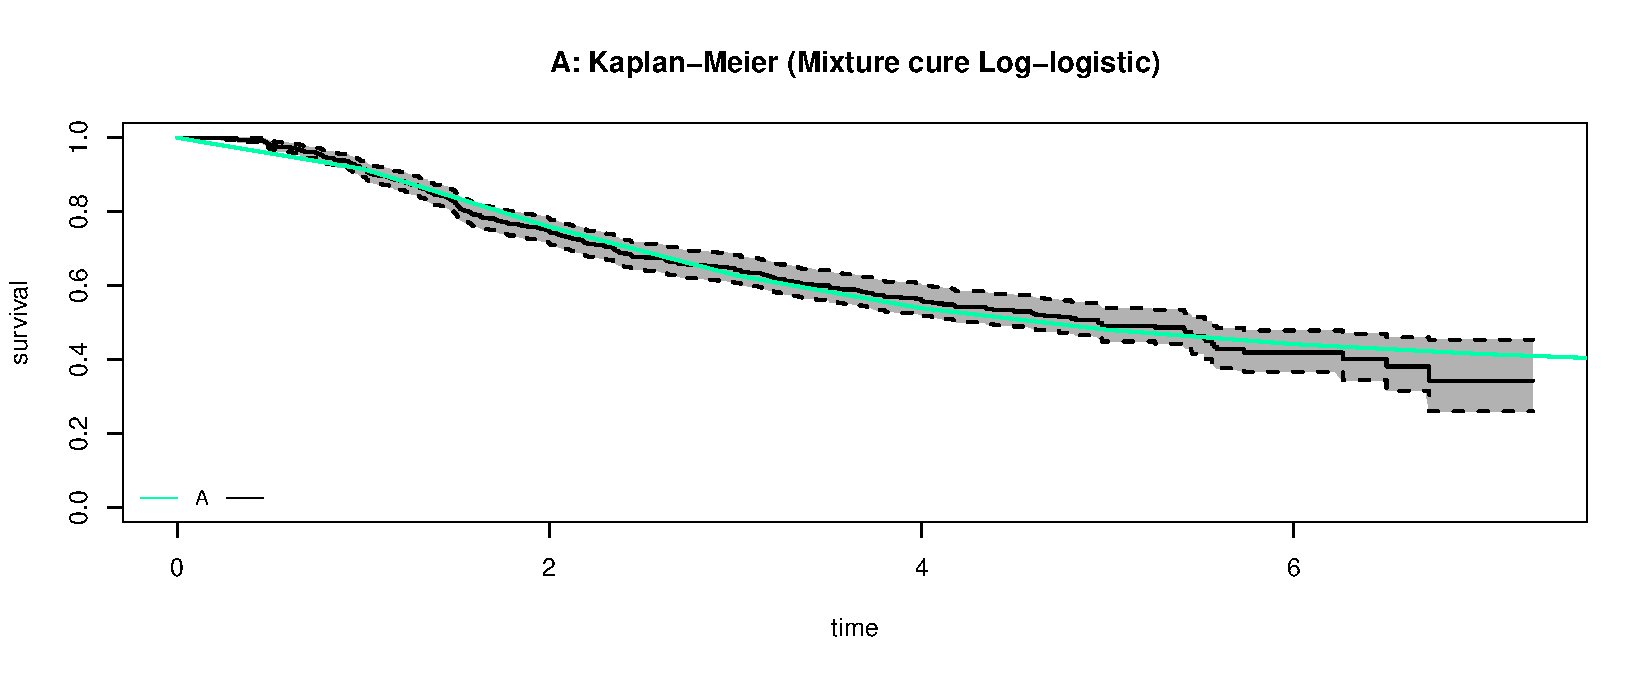
\includegraphics[height=0.25\textheight]{C:/Users/g10028783/Downloads/R talks/PERSUADE//tests/testthat/grid_test/check_20_output/Images/Figure_cure_models-13} \end{flushleft}

\begin{flushleft}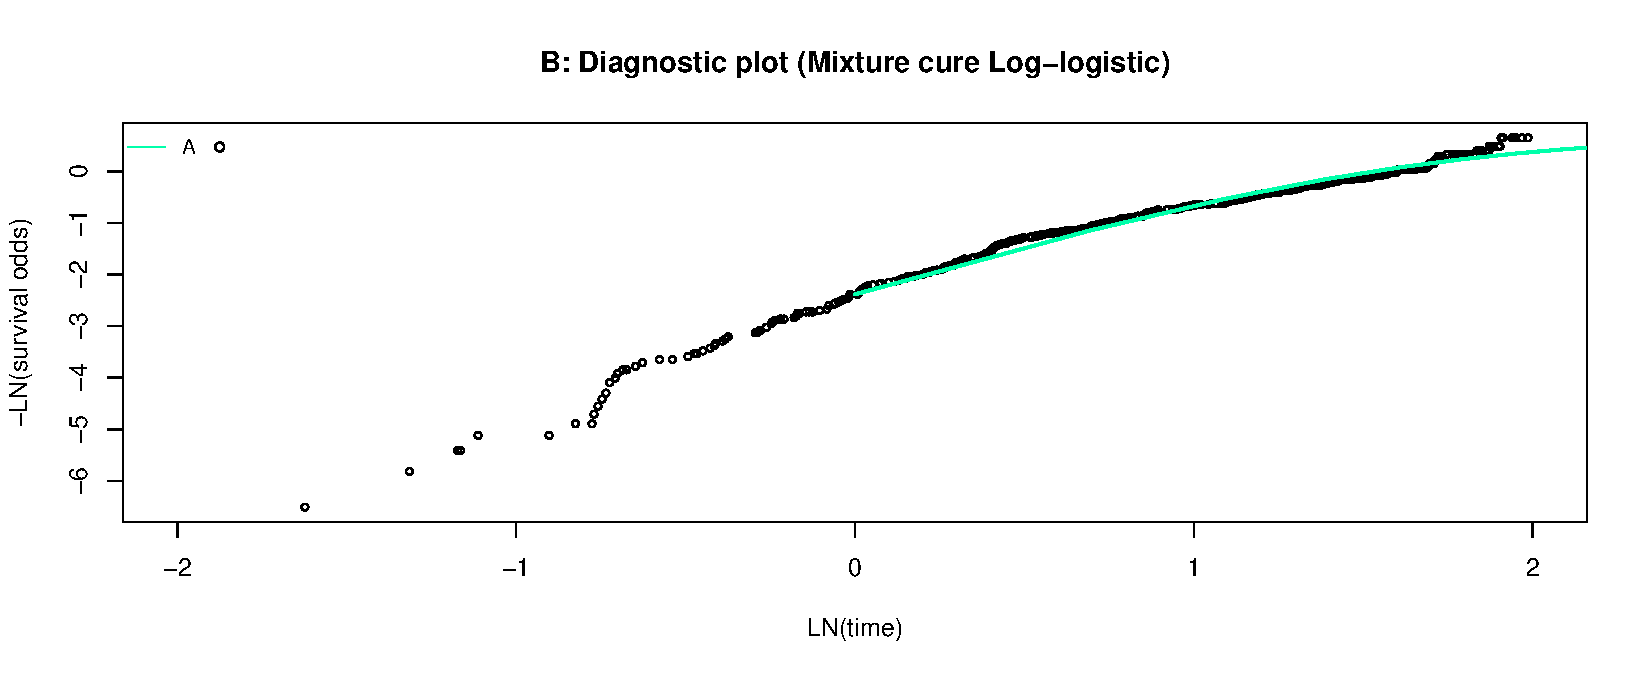
\includegraphics[height=0.25\textheight]{C:/Users/g10028783/Downloads/R talks/PERSUADE//tests/testthat/grid_test/check_20_output/Images/Figure_cure_models-14} \end{flushleft}

\begin{flushleft}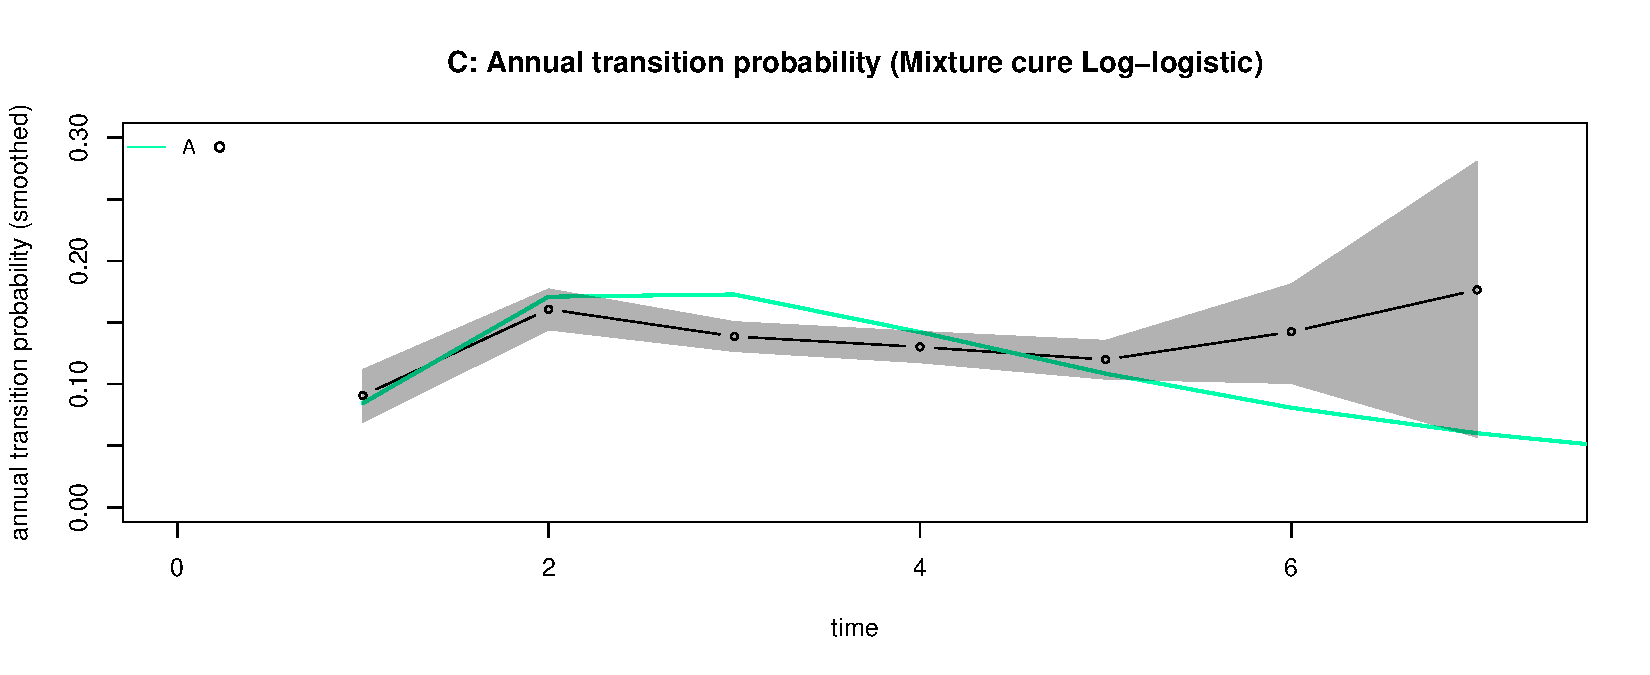
\includegraphics[height=0.25\textheight]{C:/Users/g10028783/Downloads/R talks/PERSUADE//tests/testthat/grid_test/check_20_output/Images/Figure_cure_models-15} \end{flushleft}

\clearpage

\subsubsection{Non-mixture cure
Log-logistic}\label{non-mixture-cure-log-logistic}

\begin{flushleft}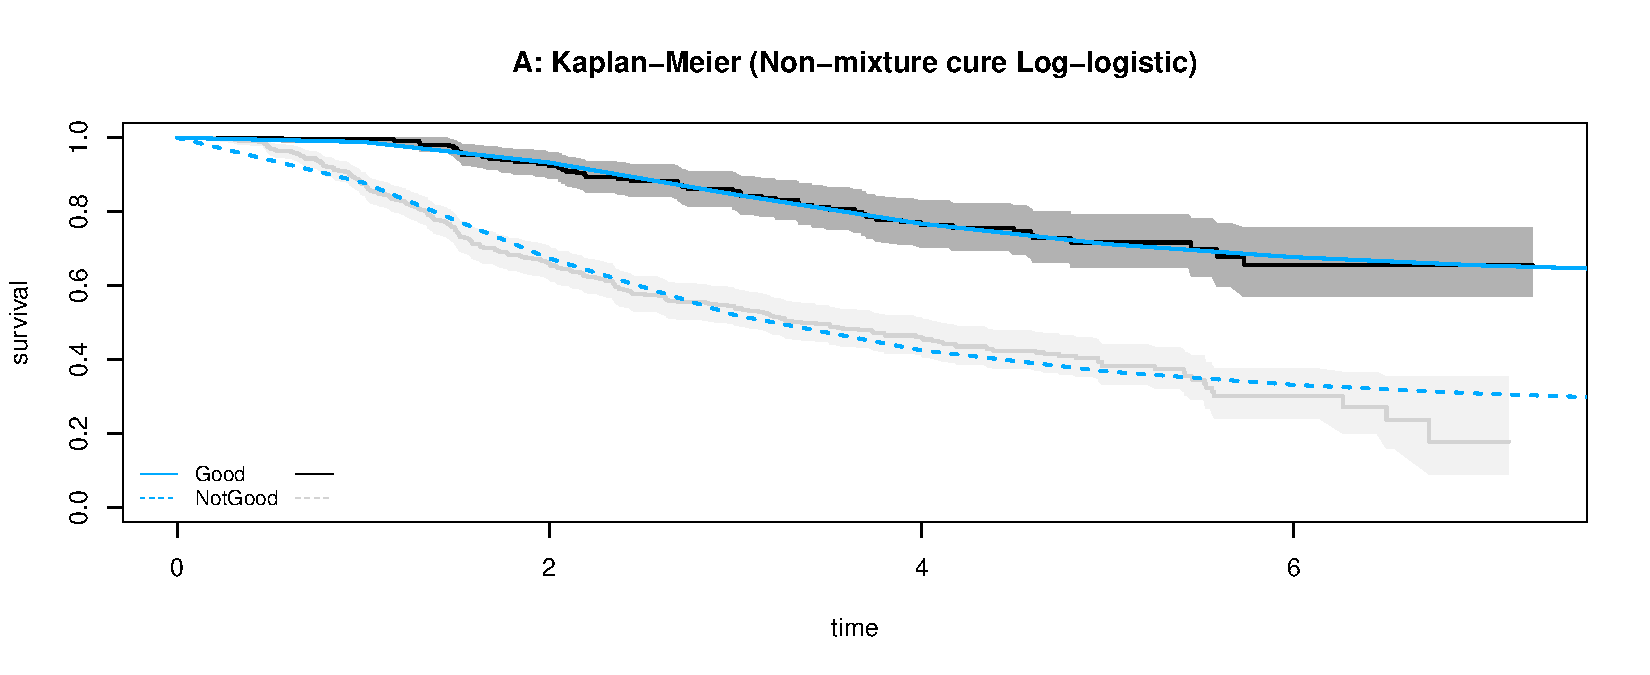
\includegraphics[height=0.25\textheight]{C:/Users/g10028783/Downloads/R talks/PERSUADE//tests/testthat/grid_test/check_20_output/Images/Figure_cure_models-16} \end{flushleft}

\begin{flushleft}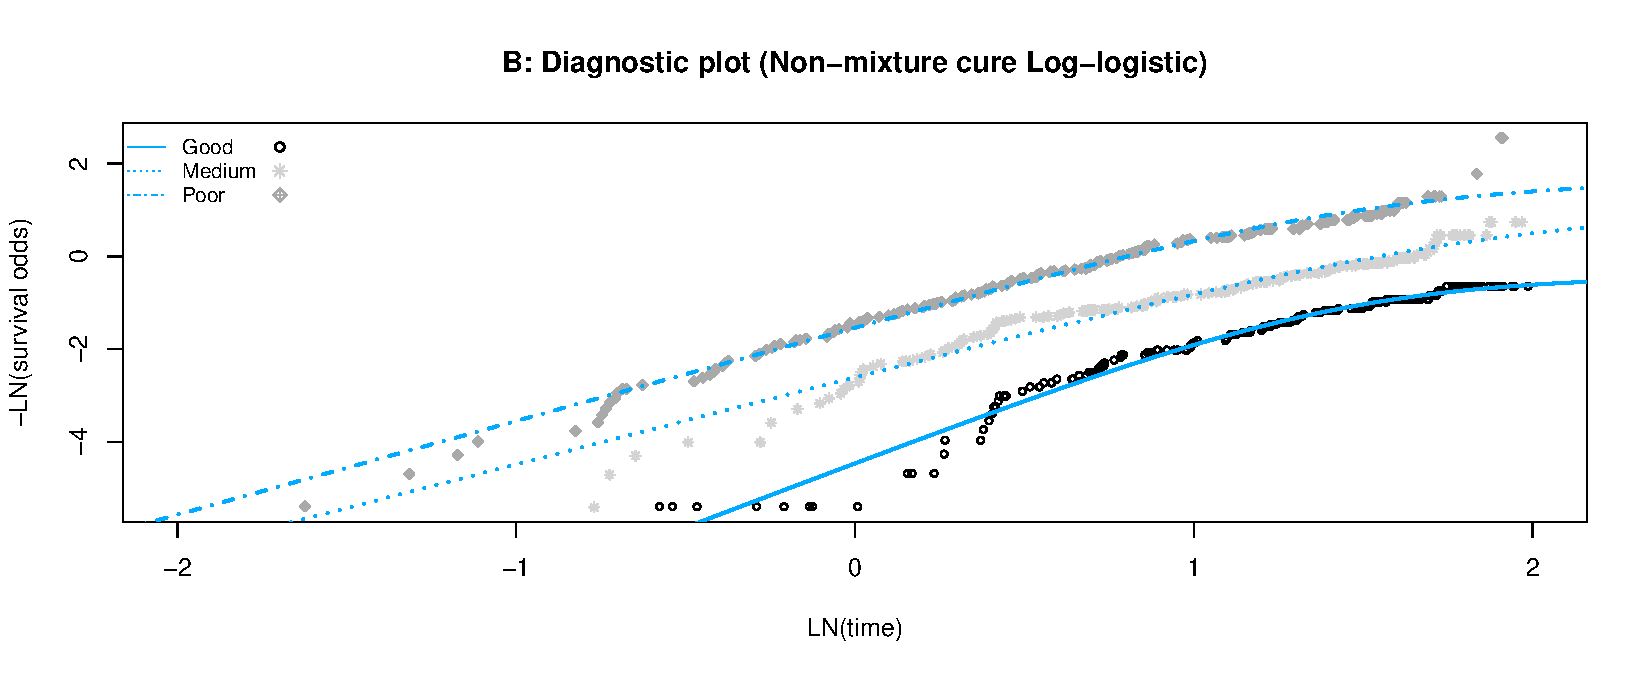
\includegraphics[height=0.25\textheight]{C:/Users/g10028783/Downloads/R talks/PERSUADE//tests/testthat/grid_test/check_20_output/Images/Figure_cure_models-17} \end{flushleft}

\begin{flushleft}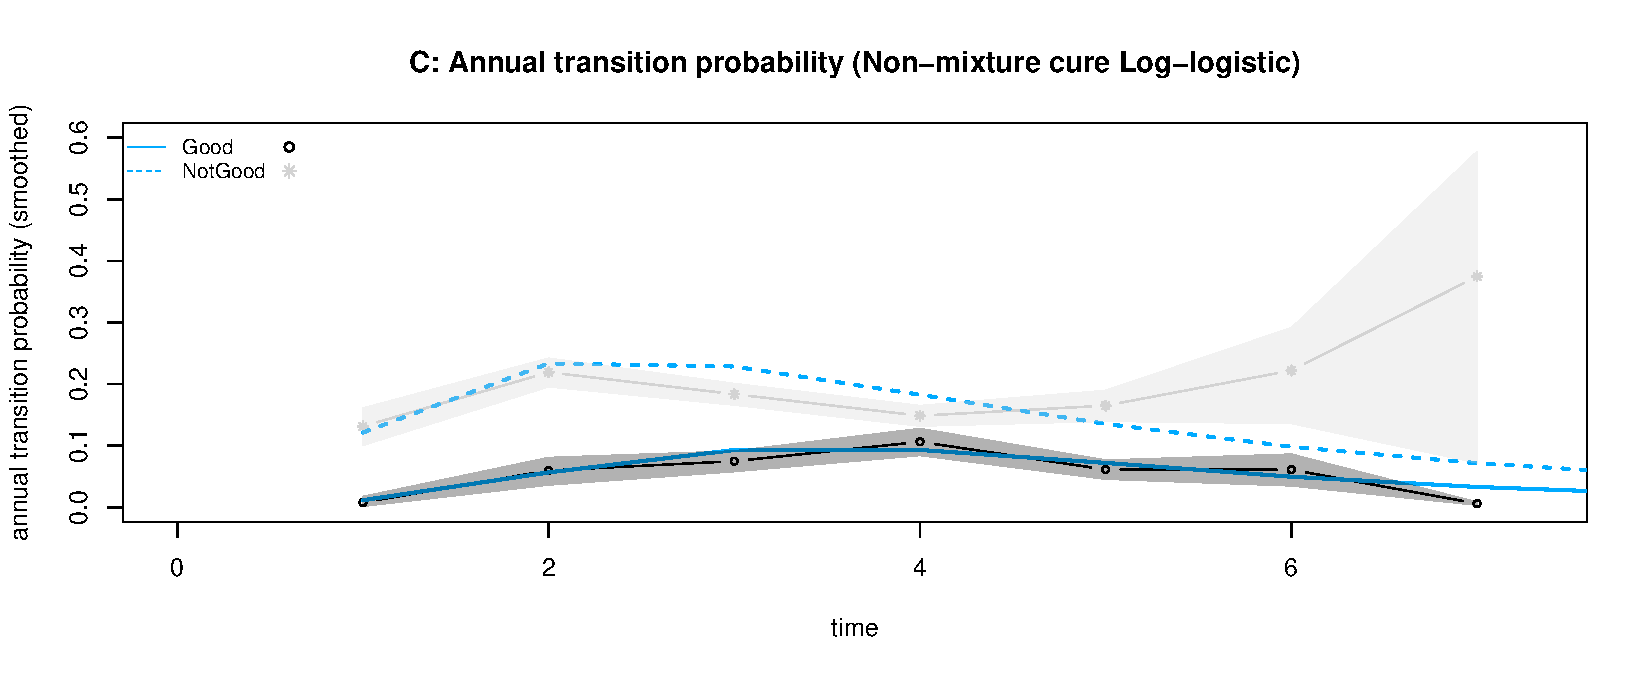
\includegraphics[height=0.25\textheight]{C:/Users/g10028783/Downloads/R talks/PERSUADE//tests/testthat/grid_test/check_20_output/Images/Figure_cure_models-18} \end{flushleft}

\clearpage

\section{5 Extrapolation}\label{extrapolation}

The plausibility of estimated survival beyond the observed data period
is often a critical driver in health economic models. As highlighted in
\href{https://nicedsu.org.uk/wp-content/uploads/2016/03/NICE-DSU-TSD-Survival-analysis.updated-March-2013.v2.pdf}{NICE
TSD 14} and \href{https://www.sheffield.ac.uk/media/34188/download}{NICE
TSD 21}, model choice for extrapolation should consider whether the
estimated long-term survival is consistent with \textbf{external data}
(e.g., observational studies, registry data, or general population
mortality).

In this section, extrapolation is examined by:

\begin{enumerate}
\def\labelenumi{\arabic{enumi}.}
\tightlist
\item
  \emph{Plotting survival curves} (Figures A) over the observed and
  extrapolated periods.\\
\item
  \emph{Plotting annual transition probabilities} (Figures B) over the
  observed and extrapolated periods.
\item
  \emph{Plotting hazard functions} (Figures C) over the observed and
  extrapolated periods.
\item
  \emph{Tabulating survival probabilities} at multiple user-specified
  time points (first table).
\item
  \emph{Summarising annual transition probabilities} (second table).
\end{enumerate}

All outputs are presented \emph{per group}.

\textbf{Assessing plausibility}

\begin{itemize}
\tightlist
\item
  Compare survival probabilities at specific time points with
  \emph{external data} (e.g., registry data, literature, expert
  opinion).\\
\item
  Compare annual transition probabilities with \emph{general population
  mortality} (e.g., from national life tables).\\
\item
  If a model predicts conditional transition probabilities more
  favourable than the general population, this may be implausible unless
  clinically justified.\\
\item
  In such cases, alternative models should be considered, or adjustments
  made (e.g., incorporating background mortality).
\end{itemize}

\textbf{Note:} These checks are consistent with the guidance in NICE TSD
14 and TSD 21, which recommend:

\begin{itemize}
\tightlist
\item
  Using \emph{external evidence} to validate extrapolations.\\
\item
  Keeping models as simple as possible (Occam's Razor), but adopting
  more flexible approaches when standard parametric models do not align
  with external evidence or long-term expectations.
\end{itemize}

\subsection{5.1 Extrapolated survival}\label{extrapolated-survival}

\begin{flushleft}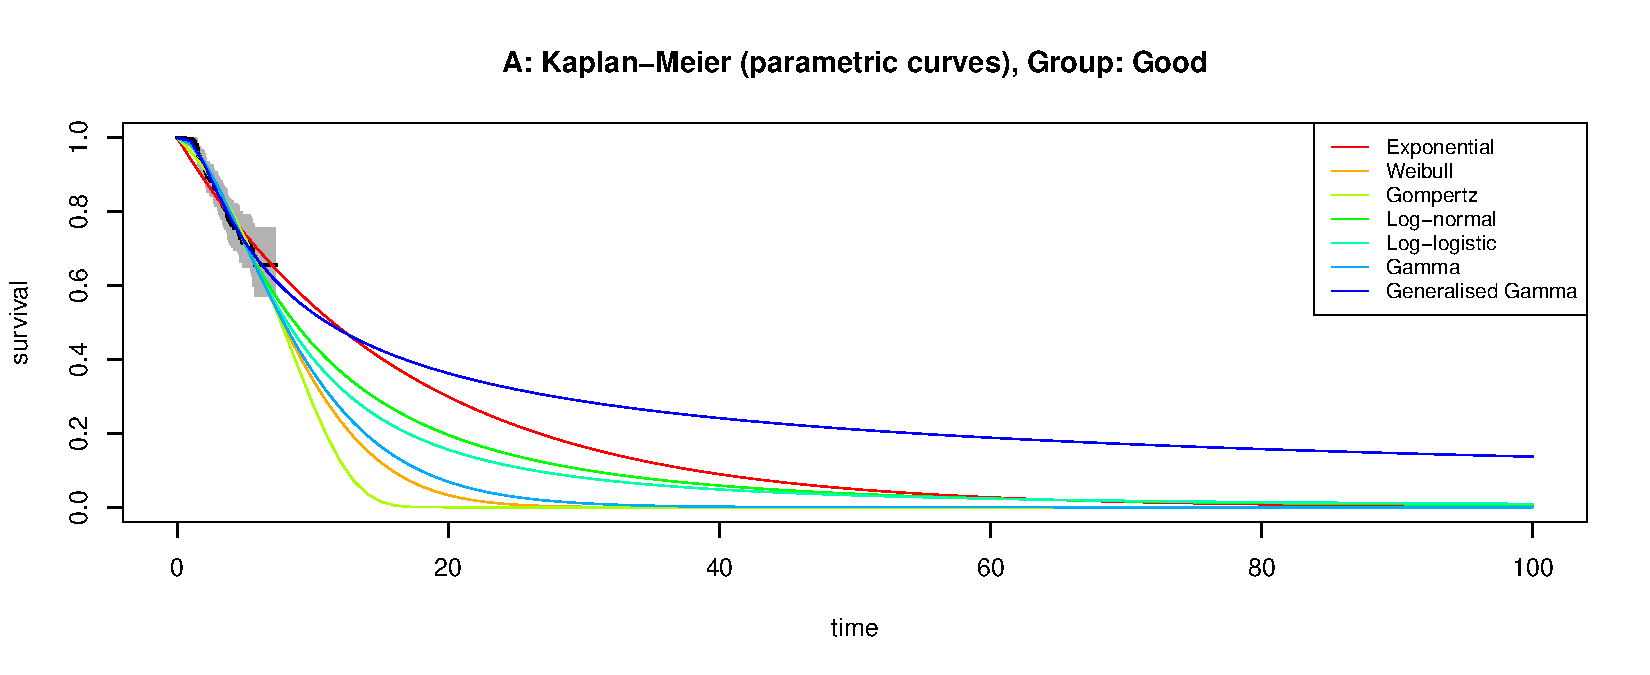
\includegraphics[height=0.29\textheight]{C:/Users/g10028783/Downloads/R talks/PERSUADE//tests/testthat/grid_test/check_20_output/Images/Figure_validate_extrapolation_KM-1} \end{flushleft}

\begin{flushleft}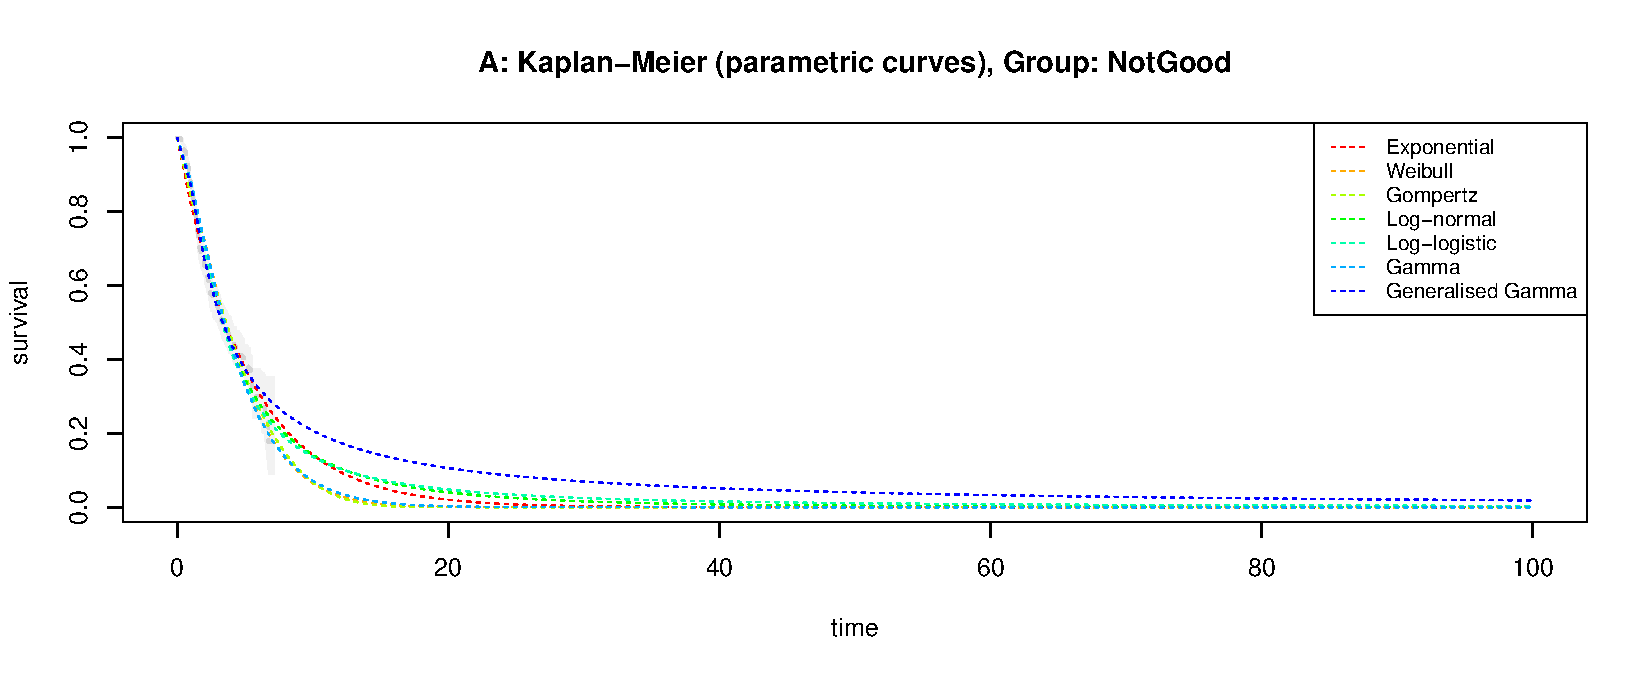
\includegraphics[height=0.29\textheight]{C:/Users/g10028783/Downloads/R talks/PERSUADE//tests/testthat/grid_test/check_20_output/Images/Figure_validate_extrapolation_KM-2} \end{flushleft}

\begin{flushleft}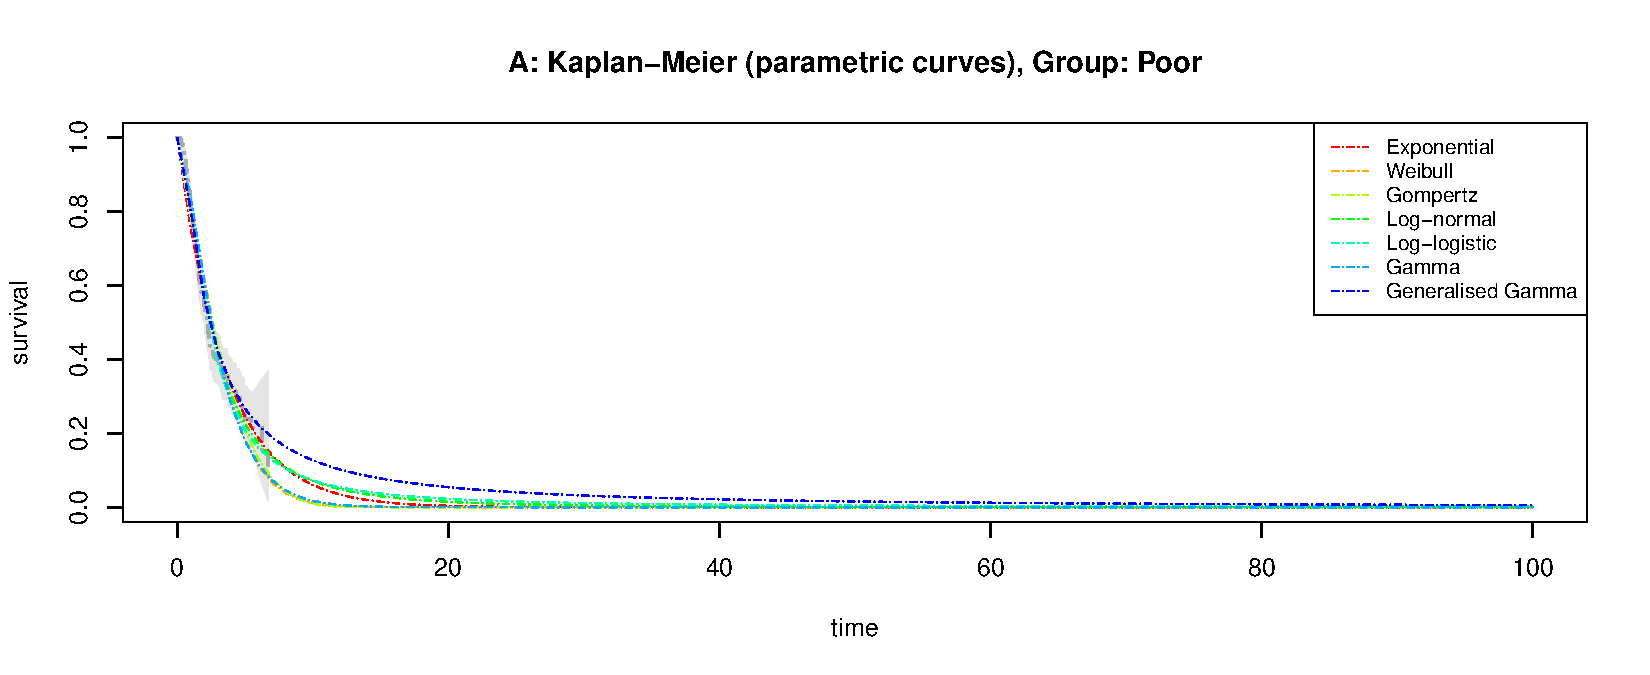
\includegraphics[height=0.29\textheight]{C:/Users/g10028783/Downloads/R talks/PERSUADE//tests/testthat/grid_test/check_20_output/Images/Figure_validate_extrapolation_KM-3} \end{flushleft}

\begin{flushleft}\includegraphics[height=0.29\textheight]{C:/Users/g10028783/Downloads/R talks/PERSUADE//tests/testthat/grid_test/check_20_output/Images/Figure_validate_extrapolation_KM-4} \end{flushleft}

\clearpage

\subsection{5.2 Extrapolated transition
probabilities}\label{extrapolated-transition-probabilities}

\begin{flushleft}\includegraphics[height=0.29\textheight]{C:/Users/g10028783/Downloads/R talks/PERSUADE//tests/testthat/grid_test/check_20_output/Images/Figure_validate_extrapolation_tp-1} \end{flushleft}

\begin{flushleft}\includegraphics[height=0.29\textheight]{C:/Users/g10028783/Downloads/R talks/PERSUADE//tests/testthat/grid_test/check_20_output/Images/Figure_validate_extrapolation_tp-2} \end{flushleft}

\begin{flushleft}\includegraphics[height=0.29\textheight]{C:/Users/g10028783/Downloads/R talks/PERSUADE//tests/testthat/grid_test/check_20_output/Images/Figure_validate_extrapolation_tp-3} \end{flushleft}

\begin{flushleft}\includegraphics[height=0.29\textheight]{C:/Users/g10028783/Downloads/R talks/PERSUADE//tests/testthat/grid_test/check_20_output/Images/Figure_validate_extrapolation_tp-4} \end{flushleft}

\clearpage

\subsection{5.3 Extrapolated hazard
function}\label{extrapolated-hazard-function}

\begin{flushleft}\includegraphics[height=0.29\textheight]{C:/Users/g10028783/Downloads/R talks/PERSUADE//tests/testthat/grid_test/check_20_output/Images/Figure_validate_extrapolation_hr-1} \end{flushleft}

\begin{flushleft}\includegraphics[height=0.29\textheight]{C:/Users/g10028783/Downloads/R talks/PERSUADE//tests/testthat/grid_test/check_20_output/Images/Figure_validate_extrapolation_hr-2} \end{flushleft}

\begin{flushleft}\includegraphics[height=0.29\textheight]{C:/Users/g10028783/Downloads/R talks/PERSUADE//tests/testthat/grid_test/check_20_output/Images/Figure_validate_extrapolation_hr-3} \end{flushleft}

\begin{flushleft}\includegraphics[height=0.29\textheight]{C:/Users/g10028783/Downloads/R talks/PERSUADE//tests/testthat/grid_test/check_20_output/Images/Figure_validate_extrapolation_hr-4} \end{flushleft}

\clearpage

\subsection{5.4 Tabulated results}\label{tabulated-results}

\subsubsection{Group Good}\label{group-good}

\begin{table}[H]
\centering
\caption{\label{tab:Table_6_1}Survival probability at different time points}
\centering
\resizebox{\ifdim\width>\linewidth\linewidth\else\width\fi}{!}{
\begin{tabular}[t]{lrrrrrrrrrrr}
\toprule
  & T= 0 & T= 10 & T= 20 & T= 30 & T= 40 & T= 50 & T= 60 & T= 70 & T= 80 & T= 90 & T= 100\\
\midrule
\cellcolor{gray!10}{Exponential} & \cellcolor{gray!10}{1} & \cellcolor{gray!10}{0.547} & \cellcolor{gray!10}{0.299} & \cellcolor{gray!10}{0.163} & \cellcolor{gray!10}{0.089} & \cellcolor{gray!10}{0.049} & \cellcolor{gray!10}{0.027} & \cellcolor{gray!10}{0.015} & \cellcolor{gray!10}{0.008} & \cellcolor{gray!10}{0.004} & \cellcolor{gray!10}{0.002}\\
Weibull & 1 & 0.452 & 0.137 & 0.033 & 0.007 & 0.001 & 0.000 & 0.000 & 0.000 & 0.000 & 0.000\\
\cellcolor{gray!10}{Gompertz} & \cellcolor{gray!10}{1} & \cellcolor{gray!10}{0.445} & \cellcolor{gray!10}{0.054} & \cellcolor{gray!10}{0.000} & \cellcolor{gray!10}{0.000} & \cellcolor{gray!10}{0.000} & \cellcolor{gray!10}{0.000} & \cellcolor{gray!10}{0.000} & \cellcolor{gray!10}{0.000} & \cellcolor{gray!10}{0.000} & \cellcolor{gray!10}{0.000}\\
Log-normal & 1 & 0.461 & 0.220 & 0.121 & 0.074 & 0.048 & 0.032 & 0.023 & 0.017 & 0.013 & 0.010\\
\cellcolor{gray!10}{Log-logistic} & \cellcolor{gray!10}{1} & \cellcolor{gray!10}{0.450} & \cellcolor{gray!10}{0.206} & \cellcolor{gray!10}{0.117} & \cellcolor{gray!10}{0.076} & \cellcolor{gray!10}{0.054} & \cellcolor{gray!10}{0.040} & \cellcolor{gray!10}{0.032} & \cellcolor{gray!10}{0.025} & \cellcolor{gray!10}{0.021} & \cellcolor{gray!10}{0.018}\\
Gamma & 1 & 0.439 & 0.137 & 0.039 & 0.010 & 0.003 & 0.001 & 0.000 & 0.000 & 0.000 & 0.000\\
\cellcolor{gray!10}{Generalised Gamma} & \cellcolor{gray!10}{1} & \cellcolor{gray!10}{0.471} & \cellcolor{gray!10}{0.276} & \cellcolor{gray!10}{0.192} & \cellcolor{gray!10}{0.146} & \cellcolor{gray!10}{0.117} & \cellcolor{gray!10}{0.097} & \cellcolor{gray!10}{0.083} & \cellcolor{gray!10}{0.072} & \cellcolor{gray!10}{0.064} & \cellcolor{gray!10}{0.057}\\
Mixture cure Weibull & 1 & 0.652 & 0.652 & 0.652 & 0.652 & 0.652 & 0.652 & 0.652 & 0.652 & 0.652 & 0.652\\
\cellcolor{gray!10}{Non-mixture cure Weibull} & \cellcolor{gray!10}{1} & \cellcolor{gray!10}{0.649} & \cellcolor{gray!10}{0.649} & \cellcolor{gray!10}{0.649} & \cellcolor{gray!10}{0.649} & \cellcolor{gray!10}{0.649} & \cellcolor{gray!10}{0.649} & \cellcolor{gray!10}{0.649} & \cellcolor{gray!10}{0.649} & \cellcolor{gray!10}{0.649} & \cellcolor{gray!10}{0.649}\\
Mixture cure Log-normal & 1 & 0.600 & 0.573 & 0.571 & 0.571 & 0.571 & 0.571 & 0.571 & 0.571 & 0.571 & 0.571\\
\cellcolor{gray!10}{Non-mixture cure Log-normal} & \cellcolor{gray!10}{1} & \cellcolor{gray!10}{0.598} & \cellcolor{gray!10}{0.564} & \cellcolor{gray!10}{0.561} & \cellcolor{gray!10}{0.561} & \cellcolor{gray!10}{0.560} & \cellcolor{gray!10}{0.560} & \cellcolor{gray!10}{0.560} & \cellcolor{gray!10}{0.560} & \cellcolor{gray!10}{0.560} & \cellcolor{gray!10}{0.560}\\
Mixture cure Log-logistic & 1 & 0.624 & 0.606 & 0.604 & 0.604 & 0.604 & 0.604 & 0.604 & 0.603 & 0.603 & 0.603\\
\cellcolor{gray!10}{Non-mixture cure Log-logistic} & \cellcolor{gray!10}{1} & \cellcolor{gray!10}{0.624} & \cellcolor{gray!10}{0.607} & \cellcolor{gray!10}{0.605} & \cellcolor{gray!10}{0.604} & \cellcolor{gray!10}{0.604} & \cellcolor{gray!10}{0.604} & \cellcolor{gray!10}{0.604} & \cellcolor{gray!10}{0.604} & \cellcolor{gray!10}{0.604} & \cellcolor{gray!10}{0.604}\\
\bottomrule
\end{tabular}}
\end{table}

\begin{table}[H]
\centering
\caption{\label{tab:Table_7_1}Summary statistics of annual transition probabilities}
\centering
\resizebox{\ifdim\width>\linewidth\linewidth\else\width\fi}{!}{
\begin{tabular}[t]{lrrrrrrrr}
\toprule
  & Mean & Std.Dev & Min & Q1 & Median & Q3 & Max & IQR\\
\midrule
\cellcolor{gray!10}{Exponential} & \cellcolor{gray!10}{0.059} & \cellcolor{gray!10}{0.000} & \cellcolor{gray!10}{0.059} & \cellcolor{gray!10}{0.059} & \cellcolor{gray!10}{0.059} & \cellcolor{gray!10}{0.059} & \cellcolor{gray!10}{0.059} & \cellcolor{gray!10}{0.000}\\
Weibull & 0.153 & 0.036 & 0.037 & 0.132 & 0.162 & 0.182 & 0.198 & 0.050\\
\cellcolor{gray!10}{Gompertz} & \cellcolor{gray!10}{0.397} & \cellcolor{gray!10}{0.297} & \cellcolor{gray!10}{0.049} & \cellcolor{gray!10}{0.130} & \cellcolor{gray!10}{0.316} & \cellcolor{gray!10}{0.647} & \cellcolor{gray!10}{0.942} & \cellcolor{gray!10}{0.518}\\
Log-normal & 0.045 & 0.018 & 0.016 & 0.031 & 0.039 & 0.056 & 0.088 & 0.025\\
\cellcolor{gray!10}{Log-logistic} & \cellcolor{gray!10}{0.039} & \cellcolor{gray!10}{0.023} & \cellcolor{gray!10}{0.016} & \cellcolor{gray!10}{0.021} & \cellcolor{gray!10}{0.030} & \cellcolor{gray!10}{0.053} & \cellcolor{gray!10}{0.091} & \cellcolor{gray!10}{0.031}\\
Gamma & 0.120 & 0.017 & 0.030 & 0.119 & 0.126 & 0.129 & 0.130 & 0.010\\
\cellcolor{gray!10}{Generalised Gamma} & \cellcolor{gray!10}{0.028} & \cellcolor{gray!10}{0.021} & \cellcolor{gray!10}{0.008} & \cellcolor{gray!10}{0.014} & \cellcolor{gray!10}{0.020} & \cellcolor{gray!10}{0.034} & \cellcolor{gray!10}{0.092} & \cellcolor{gray!10}{0.020}\\
Mixture cure Weibull & 0.004 & 0.017 & 0.000 & 0.000 & 0.000 & 0.000 & 0.097 & 0.000\\
\cellcolor{gray!10}{Non-mixture cure Weibull} & \cellcolor{gray!10}{0.004} & \cellcolor{gray!10}{0.017} & \cellcolor{gray!10}{0.000} & \cellcolor{gray!10}{0.000} & \cellcolor{gray!10}{0.000} & \cellcolor{gray!10}{0.000} & \cellcolor{gray!10}{0.097} & \cellcolor{gray!10}{0.000}\\
Mixture cure Log-normal & 0.005 & 0.017 & 0.000 & 0.000 & 0.000 & 0.000 & 0.091 & 0.000\\
\cellcolor{gray!10}{Non-mixture cure Log-normal} & \cellcolor{gray!10}{0.006} & \cellcolor{gray!10}{0.017} & \cellcolor{gray!10}{0.000} & \cellcolor{gray!10}{0.000} & \cellcolor{gray!10}{0.000} & \cellcolor{gray!10}{0.000} & \cellcolor{gray!10}{0.091} & \cellcolor{gray!10}{0.000}\\
Mixture cure Log-logistic & 0.005 & 0.017 & 0.000 & 0.000 & 0.000 & 0.000 & 0.093 & 0.000\\
\cellcolor{gray!10}{Non-mixture cure Log-logistic} & \cellcolor{gray!10}{0.005} & \cellcolor{gray!10}{0.017} & \cellcolor{gray!10}{0.000} & \cellcolor{gray!10}{0.000} & \cellcolor{gray!10}{0.000} & \cellcolor{gray!10}{0.000} & \cellcolor{gray!10}{0.093} & \cellcolor{gray!10}{0.000}\\
\bottomrule
\end{tabular}}
\end{table}

\clearpage

\subsubsection{Group NotGood}\label{group-notgood}

\begin{table}[H]
\centering
\caption{\label{tab:Table_6_2}Survival probability at different time points}
\centering
\resizebox{\ifdim\width>\linewidth\linewidth\else\width\fi}{!}{
\begin{tabular}[t]{lrrrrrrrrrrr}
\toprule
  & T= 0 & T= 10 & T= 20 & T= 30 & T= 40 & T= 50 & T= 60 & T= 70 & T= 80 & T= 90 & T= 100\\
\midrule
\cellcolor{gray!10}{Exponential} & \cellcolor{gray!10}{1} & \cellcolor{gray!10}{0.142} & \cellcolor{gray!10}{0.020} & \cellcolor{gray!10}{0.003} & \cellcolor{gray!10}{0.000} & \cellcolor{gray!10}{0.000} & \cellcolor{gray!10}{0.000} & \cellcolor{gray!10}{0.000} & \cellcolor{gray!10}{0.000} & \cellcolor{gray!10}{0.000} & \cellcolor{gray!10}{0.000}\\
Weibull & 1 & 0.065 & 0.001 & 0.000 & 0.000 & 0.000 & 0.000 & 0.000 & 0.000 & 0.000 & 0.000\\
\cellcolor{gray!10}{Gompertz} & \cellcolor{gray!10}{1} & \cellcolor{gray!10}{0.067} & \cellcolor{gray!10}{0.000} & \cellcolor{gray!10}{0.000} & \cellcolor{gray!10}{0.000} & \cellcolor{gray!10}{0.000} & \cellcolor{gray!10}{0.000} & \cellcolor{gray!10}{0.000} & \cellcolor{gray!10}{0.000} & \cellcolor{gray!10}{0.000} & \cellcolor{gray!10}{0.000}\\
Log-normal & 1 & 0.142 & 0.040 & 0.016 & 0.008 & 0.004 & 0.002 & 0.001 & 0.001 & 0.001 & 0.000\\
\cellcolor{gray!10}{Log-logistic} & \cellcolor{gray!10}{1} & \cellcolor{gray!10}{0.136} & \cellcolor{gray!10}{0.048} & \cellcolor{gray!10}{0.025} & \cellcolor{gray!10}{0.016} & \cellcolor{gray!10}{0.011} & \cellcolor{gray!10}{0.008} & \cellcolor{gray!10}{0.006} & \cellcolor{gray!10}{0.005} & \cellcolor{gray!10}{0.004} & \cellcolor{gray!10}{0.003}\\
Gamma & 1 & 0.071 & 0.003 & 0.000 & 0.000 & 0.000 & 0.000 & 0.000 & 0.000 & 0.000 & 0.000\\
\cellcolor{gray!10}{Generalised Gamma} & \cellcolor{gray!10}{1} & \cellcolor{gray!10}{0.207} & \cellcolor{gray!10}{0.106} & \cellcolor{gray!10}{0.070} & \cellcolor{gray!10}{0.051} & \cellcolor{gray!10}{0.040} & \cellcolor{gray!10}{0.033} & \cellcolor{gray!10}{0.028} & \cellcolor{gray!10}{0.024} & \cellcolor{gray!10}{0.021} & \cellcolor{gray!10}{0.019}\\
Mixture cure Weibull & 1 & 0.268 & 0.266 & 0.266 & 0.266 & 0.266 & 0.266 & 0.266 & 0.266 & 0.266 & 0.266\\
\cellcolor{gray!10}{Non-mixture cure Weibull} & \cellcolor{gray!10}{1} & \cellcolor{gray!10}{0.260} & \cellcolor{gray!10}{0.256} & \cellcolor{gray!10}{0.256} & \cellcolor{gray!10}{0.256} & \cellcolor{gray!10}{0.256} & \cellcolor{gray!10}{0.256} & \cellcolor{gray!10}{0.256} & \cellcolor{gray!10}{0.256} & \cellcolor{gray!10}{0.256} & \cellcolor{gray!10}{0.256}\\
Mixture cure Log-normal & 1 & 0.231 & 0.188 & 0.182 & 0.180 & 0.180 & 0.179 & 0.179 & 0.179 & 0.179 & 0.179\\
\cellcolor{gray!10}{Non-mixture cure Log-normal} & \cellcolor{gray!10}{1} & \cellcolor{gray!10}{0.241} & \cellcolor{gray!10}{0.191} & \cellcolor{gray!10}{0.180} & \cellcolor{gray!10}{0.176} & \cellcolor{gray!10}{0.175} & \cellcolor{gray!10}{0.174} & \cellcolor{gray!10}{0.174} & \cellcolor{gray!10}{0.173} & \cellcolor{gray!10}{0.173} & \cellcolor{gray!10}{0.173}\\
Mixture cure Log-logistic & 1 & 0.261 & 0.229 & 0.222 & 0.220 & 0.219 & 0.219 & 0.218 & 0.218 & 0.218 & 0.218\\
\cellcolor{gray!10}{Non-mixture cure Log-logistic} & \cellcolor{gray!10}{1} & \cellcolor{gray!10}{0.271} & \cellcolor{gray!10}{0.242} & \cellcolor{gray!10}{0.236} & \cellcolor{gray!10}{0.234} & \cellcolor{gray!10}{0.233} & \cellcolor{gray!10}{0.232} & \cellcolor{gray!10}{0.232} & \cellcolor{gray!10}{0.232} & \cellcolor{gray!10}{0.232} & \cellcolor{gray!10}{0.231}\\
\bottomrule
\end{tabular}}
\end{table}

\begin{table}[H]
\centering
\caption{\label{tab:Table_7_2}Summary statistics of annual transition probabilities}
\centering
\resizebox{\ifdim\width>\linewidth\linewidth\else\width\fi}{!}{
\begin{tabular}[t]{lrrrrrrrr}
\toprule
  & Mean & Std.Dev & Min & Q1 & Median & Q3 & Max & IQR\\
\midrule
\cellcolor{gray!10}{Exponential} & \cellcolor{gray!10}{0.178} & \cellcolor{gray!10}{0.000} & \cellcolor{gray!10}{0.178} & \cellcolor{gray!10}{0.178} & \cellcolor{gray!10}{0.178} & \cellcolor{gray!10}{0.178} & \cellcolor{gray!10}{0.178} & \cellcolor{gray!10}{0.000}\\
Weibull & 0.393 & 0.097 & 0.000 & 0.350 & 0.418 & 0.459 & 0.600 & 0.109\\
\cellcolor{gray!10}{Gompertz} & \cellcolor{gray!10}{0.518} & \cellcolor{gray!10}{0.257} & \cellcolor{gray!10}{0.155} & \cellcolor{gray!10}{0.288} & \cellcolor{gray!10}{0.494} & \cellcolor{gray!10}{0.744} & \cellcolor{gray!10}{0.935} & \cellcolor{gray!10}{0.457}\\
Log-normal & 0.073 & 0.044 & 0.034 & 0.042 & 0.056 & 0.087 & 0.217 & 0.045\\
\cellcolor{gray!10}{Log-logistic} & \cellcolor{gray!10}{0.054} & \cellcolor{gray!10}{0.050} & \cellcolor{gray!10}{0.016} & \cellcolor{gray!10}{0.022} & \cellcolor{gray!10}{0.032} & \cellcolor{gray!10}{0.061} & \cellcolor{gray!10}{0.227} & \cellcolor{gray!10}{0.040}\\
Gamma & 0.291 & 0.026 & 0.114 & 0.292 & 0.299 & 0.302 & 0.333 & 0.010\\
\cellcolor{gray!10}{Generalised Gamma} & \cellcolor{gray!10}{0.038} & \cellcolor{gray!10}{0.041} & \cellcolor{gray!10}{0.011} & \cellcolor{gray!10}{0.015} & \cellcolor{gray!10}{0.022} & \cellcolor{gray!10}{0.040} & \cellcolor{gray!10}{0.231} & \cellcolor{gray!10}{0.025}\\
Mixture cure Weibull & 0.012 & 0.043 & 0.000 & 0.000 & 0.000 & 0.000 & 0.222 & 0.000\\
\cellcolor{gray!10}{Non-mixture cure Weibull} & \cellcolor{gray!10}{0.012} & \cellcolor{gray!10}{0.044} & \cellcolor{gray!10}{0.000} & \cellcolor{gray!10}{0.000} & \cellcolor{gray!10}{0.000} & \cellcolor{gray!10}{0.000} & \cellcolor{gray!10}{0.226} & \cellcolor{gray!10}{0.000}\\
Mixture cure Log-normal & 0.016 & 0.044 & 0.000 & 0.000 & 0.000 & 0.003 & 0.230 & 0.003\\
\cellcolor{gray!10}{Non-mixture cure Log-normal} & \cellcolor{gray!10}{0.016} & \cellcolor{gray!10}{0.043} & \cellcolor{gray!10}{0.000} & \cellcolor{gray!10}{0.000} & \cellcolor{gray!10}{0.001} & \cellcolor{gray!10}{0.005} & \cellcolor{gray!10}{0.236} & \cellcolor{gray!10}{0.005}\\
Mixture cure Log-logistic & 0.014 & 0.043 & 0.000 & 0.000 & 0.000 & 0.003 & 0.234 & 0.002\\
\cellcolor{gray!10}{Non-mixture cure Log-logistic} & \cellcolor{gray!10}{0.014} & \cellcolor{gray!10}{0.042} & \cellcolor{gray!10}{0.000} & \cellcolor{gray!10}{0.000} & \cellcolor{gray!10}{0.000} & \cellcolor{gray!10}{0.002} & \cellcolor{gray!10}{0.233} & \cellcolor{gray!10}{0.002}\\
\bottomrule
\end{tabular}}
\end{table}

\clearpage

\section{6. PERSUADE object
information}\label{persuade-object-information}

\begin{verbatim}
## List of 7
##  $ name            : chr "/tests/testthat/grid_test/check_20"
##  $ input           :List of 11
##   ..$ years               : num [1:686] 3.68 4.32 4.82 3.16 2.65 ...
##   ..$ status              : num [1:686] 0 0 0 0 0 0 0 1 0 0 ...
##   ..$ group               : Factor w/ 2 levels "Good","NotGood": 1 1 1 1 1 1 1 1 1 1 ...
##   ..$ strata              : logi FALSE
##   ..$ spline_mod          : logi FALSE
##   ..$ cure_mod            : logi TRUE
##   ..$ cure_link           : chr "loglog"
##   ..$ time_unit           : num 1
##   ..$ time_horizon        : num 100
##   ..$ time_pred_surv_table: num [1:11] 0 10 20 30 40 50 60 70 80 90 ...
##   ..$ time_pred           : num [1:101] 0 1 2 3 4 5 6 7 8 9 ...
##  $ surv_obs        :List of 6
##   ..$ km      :List of 24
##   .. ..- attr(*, "class")= chr [1:2] "npsurv" "survfit"
##   ..$ km_names: int [1:618] 1 1 1 1 1 1 1 1 1 1 ...
##   ..$ cum_haz :'data.frame': 16 obs. of  9 variables:
##   ..$ haz     :List of 3
##   ..$ tp      :List of 3
##   ..$ cox_reg :List of 21
##   .. ..- attr(*, "class")= chr "coxph"
##  $ surv_model      :List of 4
##   ..$ param_models:List of 7
##   ..$ param_ic    :'data.frame': 7 obs. of  3 variables:
##   ..$ cure_models :List of 6
##   ..$ cure_ic     :'data.frame': 6 obs. of  3 variables:
##  $ surv_pred       :List of 3
##   ..$ model:List of 8
##   ..$ gr   :List of 2
##   ..$ tp_gr:List of 2
##  $ surv_model_excel:'data.frame':    13 obs. of  21 variables:
##   ..$ rate        : chr [1:13] "expo" "rate" "-2.80703426596047" "-3.08148411925753" ...
##   ..$ groupNotGood: chr [1:13] "expo" "groupNotGood" "1.17461456842401" "0.873263485326394" ...
##   ..$ shape       : chr [1:13] "weib" "shape" "0.27992372335589" "0.184068542926647" ...
##   ..$ scale       : chr [1:13] "weib" "scale" "2.47644595229751" "2.24797696246046" ...
##   ..$ groupNotGood: chr [1:13] "weib" "groupNotGood" "-0.933877645137855" "-1.17311140485413" ...
##   ..$ shape       : chr [1:13] "gom" "shape" "0.0960392151564178" "0.0222985115994405" ...
##   ..$ rate        : chr [1:13] "gom" "rate" "-3.0329890248275" "-3.3626512278081" ...
##   ..$ groupNotGood: chr [1:13] "gom" "groupNotGood" "1.20672838161353" "0.904298780253262" ...
##   ..$ meanlog     : chr [1:13] "lnorm" "meanlog" "2.20255433833324" "2.00168193523675" ...
##   ..$ sdlog       : chr [1:13] "lnorm" "sdlog" "0.0246796999755503" "-0.0622573732233042" ...
##   ..$ groupNotGood: chr [1:13] "lnorm" "groupNotGood" "-1.00014914678769" "-1.2154778065186" ...
##   ..$ shape       : chr [1:13] "llog" "shape" "0.504500574328399" "0.409955855267665" ...
##   ..$ scale       : chr [1:13] "llog" "scale" "2.18072457092369" "1.97615384538411" ...
##   ..$ groupNotGood: chr [1:13] "llog" "groupNotGood" "-0.993207250544198" "-1.21644803324429" ...
##   ..$ shape       : chr [1:13] "gam" "shape" "0.466242635593982" "0.32801270711823" ...
##   ..$ rate        : chr [1:13] "gam" "rate" "-1.92971638236834" "-2.23616315126186" ...
##   ..$ groupNotGood: chr [1:13] "gam" "groupNotGood" "0.926728618387163" "0.702771447636794" ...
##   ..$ mu          : chr [1:13] "ggam" "mu" "1.92035873095608" "1.65615352381609" ...
##   ..$ sigma       : chr [1:13] "ggam" "sigma" "0.113705306856937" "0.0253043057746046" ...
##   ..$ Q           : chr [1:13] "ggam" "Q" "-0.745102030733346" "-1.2032221848416" ...
##   ..$ groupNotGood: chr [1:13] "ggam" "groupNotGood" "-1.01674071929335" "-1.21767585164945" ...
##  $ misc            :List of 6
##   ..$ form       :Class 'formula'  language survival::Surv(years, status) ~ group
##   .. .. ..- attr(*, ".Environment")=<environment: 0x0000021a4ba859e0> 
##   ..$ group_names: chr [1:2] "Good" "NotGood"
##   ..$ ngroups    : int 2
##   ..$ lbls       : chr [1:7] "Exponential" "Weibull" "Gompertz" "Log-normal" ...
##   ..$ lbls_cure  : chr [1:6] "Mixture cure Weibull" "Non-mixture cure Weibull" "Mixture cure Log-normal" "Non-mixture cure Log-normal" ...
##   ..$ cols_tp    : num 14
##  - attr(*, "class")= chr "PERSUADE"
## NULL
\end{verbatim}

\clearpage

\section{7. Session information}\label{session-information}

\begin{verbatim}
## R version 4.4.2 (2024-10-31 ucrt)
## Platform: x86_64-w64-mingw32/x64
## Running under: Windows 11 x64 (build 26100)
## 
## Matrix products: default
## 
## 
## Random number generation:
##  RNG:     Mersenne-Twister 
##  Normal:  Inversion 
##  Sample:  Rejection 
##  
## attached base packages:
## [1] stats     graphics  grDevices utils     datasets  methods   base     
## 
## other attached packages:
## [1] testthat_3.2.3      PERSUADE_0.0.0.9000
## 
## loaded via a namespace (and not attached):
##   [1] splines_4.4.2       later_1.4.2         polspline_1.1.25   
##   [4] bitops_1.0-9        tibble_3.2.1        rpart_4.1.23       
##   [7] deSolve_1.40        lifecycle_1.0.4     rstatix_0.7.2      
##  [10] rprojroot_2.0.4     processx_3.8.4      lattice_0.22-6     
##  [13] MASS_7.3-61         backports_1.5.0     magrittr_2.0.3     
##  [16] Hmisc_5.2-3         sass_0.4.10         rmarkdown_2.29     
##  [19] jquerylib_0.1.4     yaml_2.3.10         remotes_2.5.0      
##  [22] httpuv_1.6.15       flexsurvcure_1.3.3  sessioninfo_1.2.2  
##  [25] pkgbuild_1.4.5      RColorBrewer_1.1-3  multcomp_1.4-28    
##  [28] abind_1.4-8         pkgload_1.4.0       quadprog_1.5-8     
##  [31] purrr_1.0.4         RCurl_1.98-1.17     nnet_7.3-19        
##  [34] pracma_2.4.4        TH.data_1.1-3       sandwich_3.1-1     
##  [37] KMsurv_0.1-6        MatrixModels_0.5-4  svglite_2.2.1      
##  [40] commonmark_2.0.0    codetools_0.2-20    ggtext_0.1.2       
##  [43] xml2_1.4.0          tidyselect_1.2.1    SuppDists_1.1-9.9  
##  [46] farver_2.1.2        base64enc_0.1-3     jsonlite_2.0.0     
##  [49] ks_1.15.1           ellipsis_0.3.2      Formula_1.2-5      
##  [52] survival_3.7-0      systemfonts_1.2.3   tools_4.4.2        
##  [55] Rcpp_1.0.13-1       glue_1.8.0          gridExtra_2.3      
##  [58] xfun_0.52           usethis_3.0.0       dplyr_1.1.4        
##  [61] withr_3.0.2         numDeriv_2016.8-1.1 muhaz_1.2.6.4      
##  [64] fastmap_1.2.0       boot_1.3-31         mstate_0.3.3       
##  [67] SparseM_1.84-2      litedown_0.7        callr_3.7.6        
##  [70] digest_0.6.37       R6_2.6.1            mime_0.12          
##  [73] textshaping_1.0.1   colorspace_2.1-1    dichromat_2.0-0.1  
##  [76] markdown_2.0        tidyr_1.3.1         generics_0.1.4     
##  [79] data.table_1.16.4   htmlwidgets_1.6.4   pkgconfig_2.0.3    
##  [82] gtable_0.3.6        pcaPP_2.0-5         survMisc_0.5.6     
##  [85] brio_1.1.5          htmltools_0.5.8.1   carData_3.0-5      
##  [88] profvis_0.4.0       scales_1.4.0        kableExtra_1.4.0   
##  [91] knitr_1.50          km.ci_0.5-6         rstudioapi_0.17.1  
##  [94] checkmate_2.3.3     nlme_3.1-166        curl_6.4.0         
##  [97] cachem_1.1.0        zoo_1.8-14          sft_2.4            
## [100] stringr_1.5.1       KernSmooth_2.23-24  miniUI_0.1.1.1     
## [103] fda_6.3.0           foreign_0.8-87      desc_1.4.3         
## [106] pillar_1.11.0       grid_4.4.2          vctrs_0.6.5        
## [109] urlchecker_1.0.1    promises_1.3.3      ggpubr_0.6.1       
## [112] car_3.1-3           xtable_1.8-4        cluster_2.1.6      
## [115] waldo_0.6.1         htmlTable_2.4.3     evaluate_1.0.5     
## [118] tinytex_0.57        mvtnorm_1.3-3       cli_3.6.3          
## [121] compiler_4.4.2      rlang_1.1.6         rms_8.0-0          
## [124] ggsignif_0.6.4      survminer_0.5.0     labeling_0.4.3     
## [127] mclust_6.1.1        fds_1.8             ps_1.8.1           
## [130] fs_1.6.5            stringi_1.8.7       rainbow_3.8        
## [133] viridisLite_0.4.2   hdrcde_3.4          devtools_2.4.5     
## [136] quantreg_6.1        Matrix_1.7-1        ggplot2_3.5.2      
## [139] statmod_1.5.0       shiny_1.10.0        flexsurv_2.3.2     
## [142] gridtext_0.1.5      broom_1.0.9         memoise_2.0.1      
## [145] bslib_0.9.0
\end{verbatim}

\end{document}
